%7 July 2010: still missing reference to Containment and Support
%3 August 2010 Few of Dakubu's comments aren't satisfied


\chapter{Space}
\label{sec:SPA-chap}
%test school, need book with notes

\section{Introduction}
\label{sec:SPA-intro}

This chapter provides a description of the means by which Chakali encodes
spatial meaning,  with a focus on the linguistic description of static
configurations. We start by introducing some preliminary notions and the kind of
semantic components expected to be involved in the expression of this particular
type of spatial meaning. In section \ref{sec:SPA-topo-rel} I present  five
tasks which were carried out and discuss the results.  In section
\ref{sec:SPA-tr}, I
identify  Chakali's  {\it  basic locative construction} and {\it  topological
relation markers} \citep{Levi06}. Among the  topological relation markers, I
describe the grammar and usage of the relational nouns, the postposition and the
verbal component. Concerning the latter, this chapter contributes to the
typological
classification of locative predication  proposed by \cite{Amek07b}.  


\section{Background and motivation}
\label{sec:SPA-back-mot}
 
One approach to  describing how speakers of different languages
structure the spatial domain is to develop an appropriate semantic typology
using methods which explore cross-linguistic similarities and differences in
semantic terms \citep[513]{Levi06}. To provide such a framework, a semantic
typology ought to be equipped with   formal and cross-linguistically viable
notions. \cite{Jack83} is among the first to study languages in these
terms \cite[see also][]{Talm83, Hers86, Lako87, Vand91}. With his {\it
conceptual structure}, \citeauthor{Jack83} introduced an autonomous level of
representation, consisting of  primitives and principles of combination, ``onto
which and from which all peripheral information is mapped'' \citep[19]{Jack83}.
To account for spatial expressions, conceptual features (or conceptual primes)
such as [PLACE], [PATH], [THING], [DIRECTION], etc.  are structured at the
conceptual level and mapped onto a grammar and lexicon.  For instance, the
sentence  `the man stood in the room' may be represented with the conceptual
structure in (\ref{ex:SPA-jackendoff}):\footnote{\cite{Jack83} does not offer
much detail on how  posture and position predicates are represented in his
framework. However, on page 173, he offers the state-function ORIENT which may
capture the common meaning  of `stand', `lie', etc. This is our intention in
(\ref{ex:SPA-jackendoff}).}

%add Mill76 to list of studies

\begin{exe}
\ex\label{ex:SPA-jackendoff}
$[_{State}  \textnormal{ORIENT} ([_{Thing}   \textnormal{MAN}], [_{Place}  
\textnormal{IN} ([_{Thing}  \textnormal{ROOM}])])]$
\end{exe}

The conceptual features of \cite{Jack83} are more or less interpreted as
conceptual primitives by some linguists. For instance, in cognitive  semantic
terms, languages differ only with respect to how they lexicalize and compose 
the conceptual primitives \citep{Talm83, Wier96}.  Even though  
\citeauthor{Jack83}'s  conceptual  structure is intended to be
language-independent, it has
been applied mainly to account for spatial expressions  of English and
typologically similar languages.  

More recently,  many studying the relationship between language and space
 have adoptep the framework of Talmy’s typology \citep{Talm00a}. This
framework, a
series of various conceptual components, is used to encode and analyze
cross-linguistic  data in a transparent way. 

\begin{exe}
\ex\label{ex:SPA-sta-dyn}
 \begin{xlist} 
\ex\label{ex:SPA-stat-Eng}{\it Static}
\gll {[The man]} stood in {[the room]}\\
{\sc figure}  {\sc localisation} {\sc site} {\sc ground}\\
  \ex\label{ex:SPA-dyn-Eng}{\it Dynamic}
\gll  {[The man]}  fell from {[the roof]}\\
{\sc figure}  {\sc displacement} {\sc trajectory} {\sc ground}\\
 \end{xlist}
\end{exe} 


\begin{figure}[htp]
 \centering

 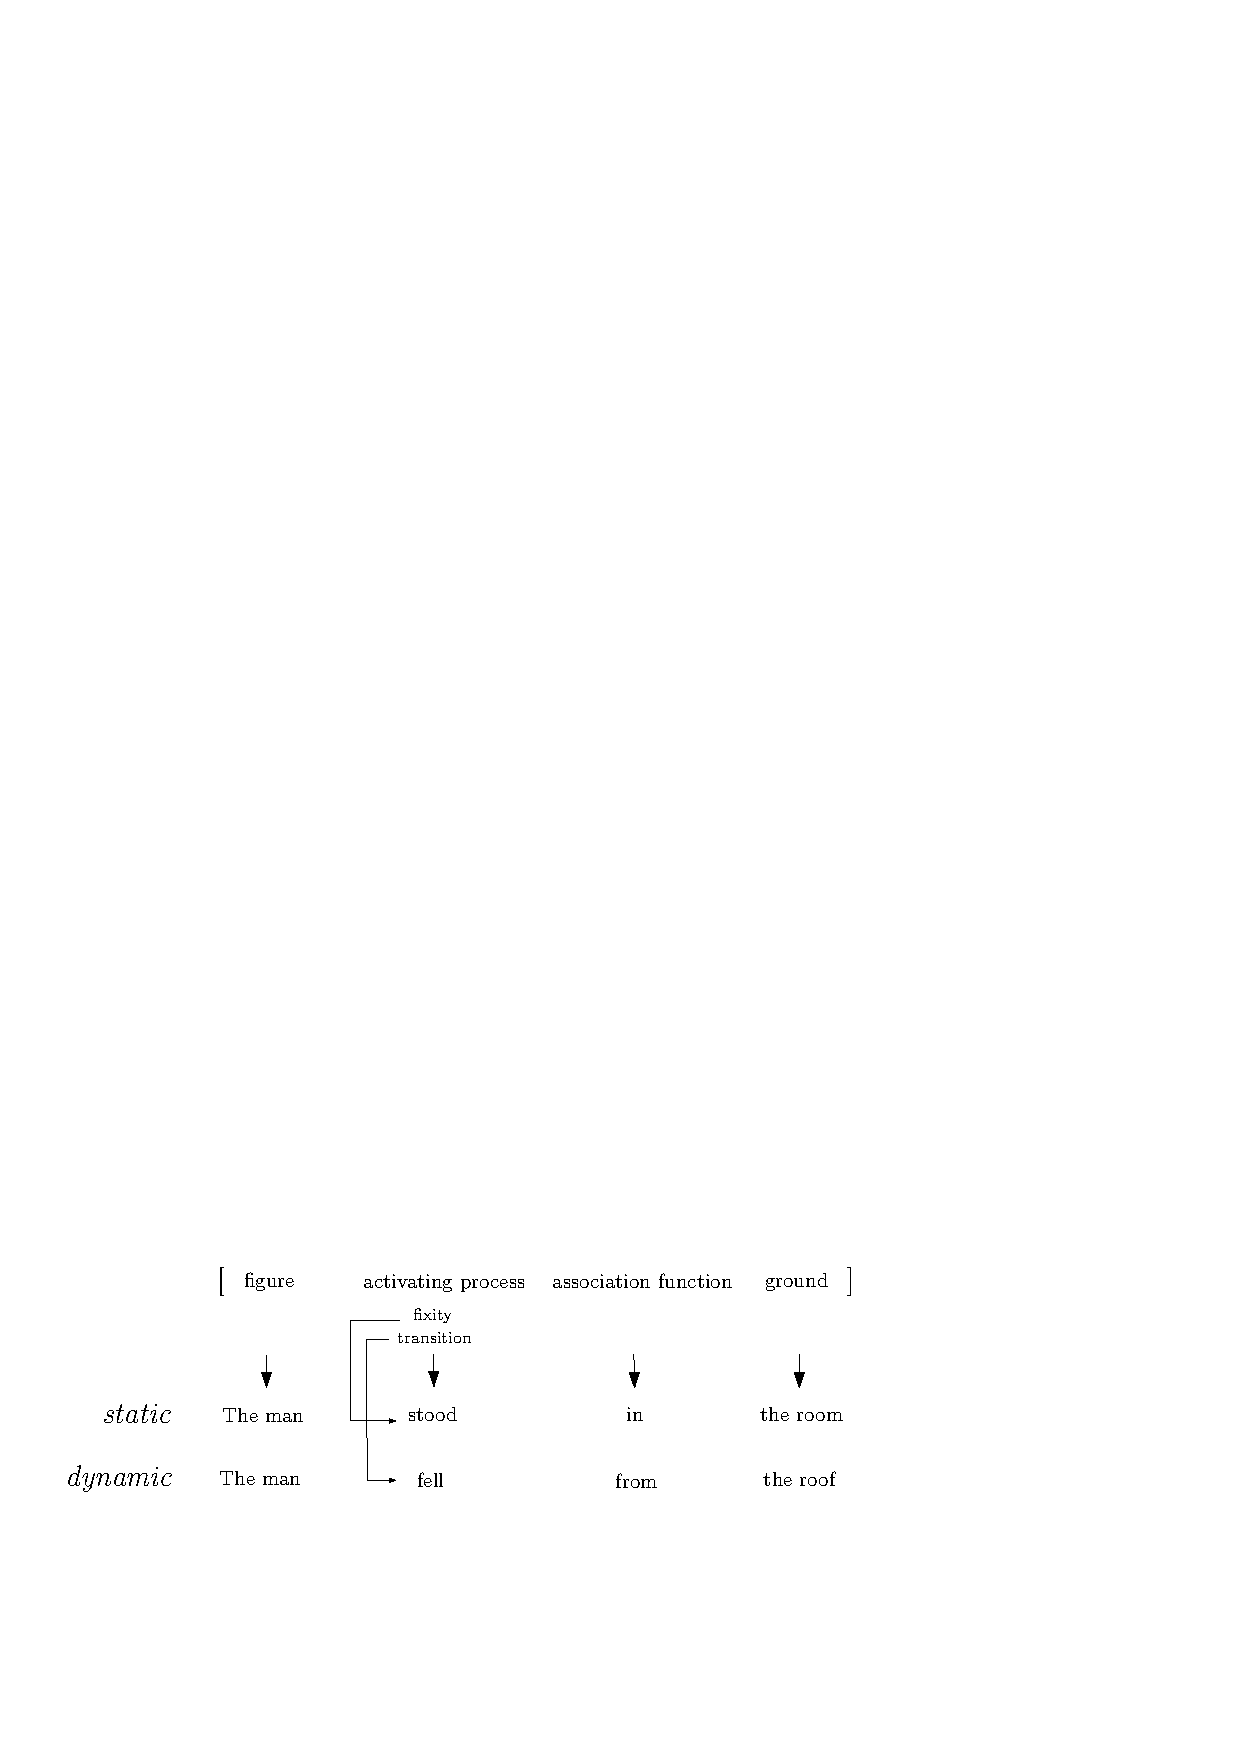
\includegraphics[width=4.5in]{Graphic/Pictures/Talmy-schema.pdf}
 % Talmy-schema.pdf: 595x842 pixel, 72dpi, 20.99x29.70 cm, bb=0 0 595 842

 \caption{Conceptual components and  structure of a locative expression in a
framing event 
\citep[221]{Talm00a}  \label{ex:SPA-Talmy}}

\end{figure}



Let us
consider example (\ref{ex:SPA-sta-dyn}) and Talmy's framing event  in
figure \ref{ex:SPA-Talmy}. 
Linguists owe the notions of  \textit{figure} and \textit{ground} to
\citet[232]{Talm83}, who himself borrowed the notions from Gestalt psychology. A
 figure, i.e. an object to be located, is located  by reference to  a ground,
i.e. an object or a spatial environment that serves as a point of
reference.\footnote{Figure and ground are  called {\it theme} and {\it reference
object} respectively in \cite{Jack83}.}  The figure is the entity which receives
the most prominent attention. Consequently, it is usually encoded as 
grammatical
subject.     The spatial relationship between figure and
ground can be either
static, i.e. where a stable and fixed position of the figure is determined,  as
in
`The man stood in the room', or dynamic, i.e.  where movement or transition of
the figure from/to the ground is determined,  as in `The man fell from the
roof'. 
\citeauthor{Talm00a} calls the activating process  the
conceptual component
where the spatial localization event is interpreted, whereas the association
function ``sets the figural entity into a particular relationship with the
ground entity'' \citep[218]{Talm00b}.  A static
relation involves a localization as
activating process and a site as association function, whereas a dynamic
relation   involves  a displacement  as  activating process and a trajectory  as
association function. 

It is believed that the grammatical encoding of what \citeauthor{Talm00a} calls
the activating process and the association function  are where languages differ
  most.   Therefore, the question to be addressed in this chapter is simple:
What are the characteristics of spatial expressions in Chakali, specifically
those involved in the description of static configurations? Since I wish to
answer this question from a typological viewpoint, the present study is  cast
in the conceptual subdivisions of spatial domain as defined in \citet{Levi06},
which I now introduce.

Over the last two decades, the spatial domain of a wide range of languages has
been studied by the Language and Cognition Group at the Max Planck Institute for
Psycholinguistics, Nijmegen. What is special about this research is the
practice of using
the same elicitation tools for the collection of data from all over the
world.\footnote{``The Language and Cognition group investigates the relationship
between language and general cognition, making use of the `natural laboratory'
of language variation. To this end, it maintains about a dozen field sites
around the world, where languages are described often for the first time, the
semantic categories examined and field experiments conducted.'' \\ {\it
http://www.mpi.nl/institute/research-groups/language-and-cognition-group}
(accessed on April 26, 2010).} My interest in their framework derives
precisely 
from the possibility of placing Chakali within a typology which is based on the
result of a standardized method for data collection, which in turn makes it
possible to compare languages reliably. 


\begin{figure}
 \centering
 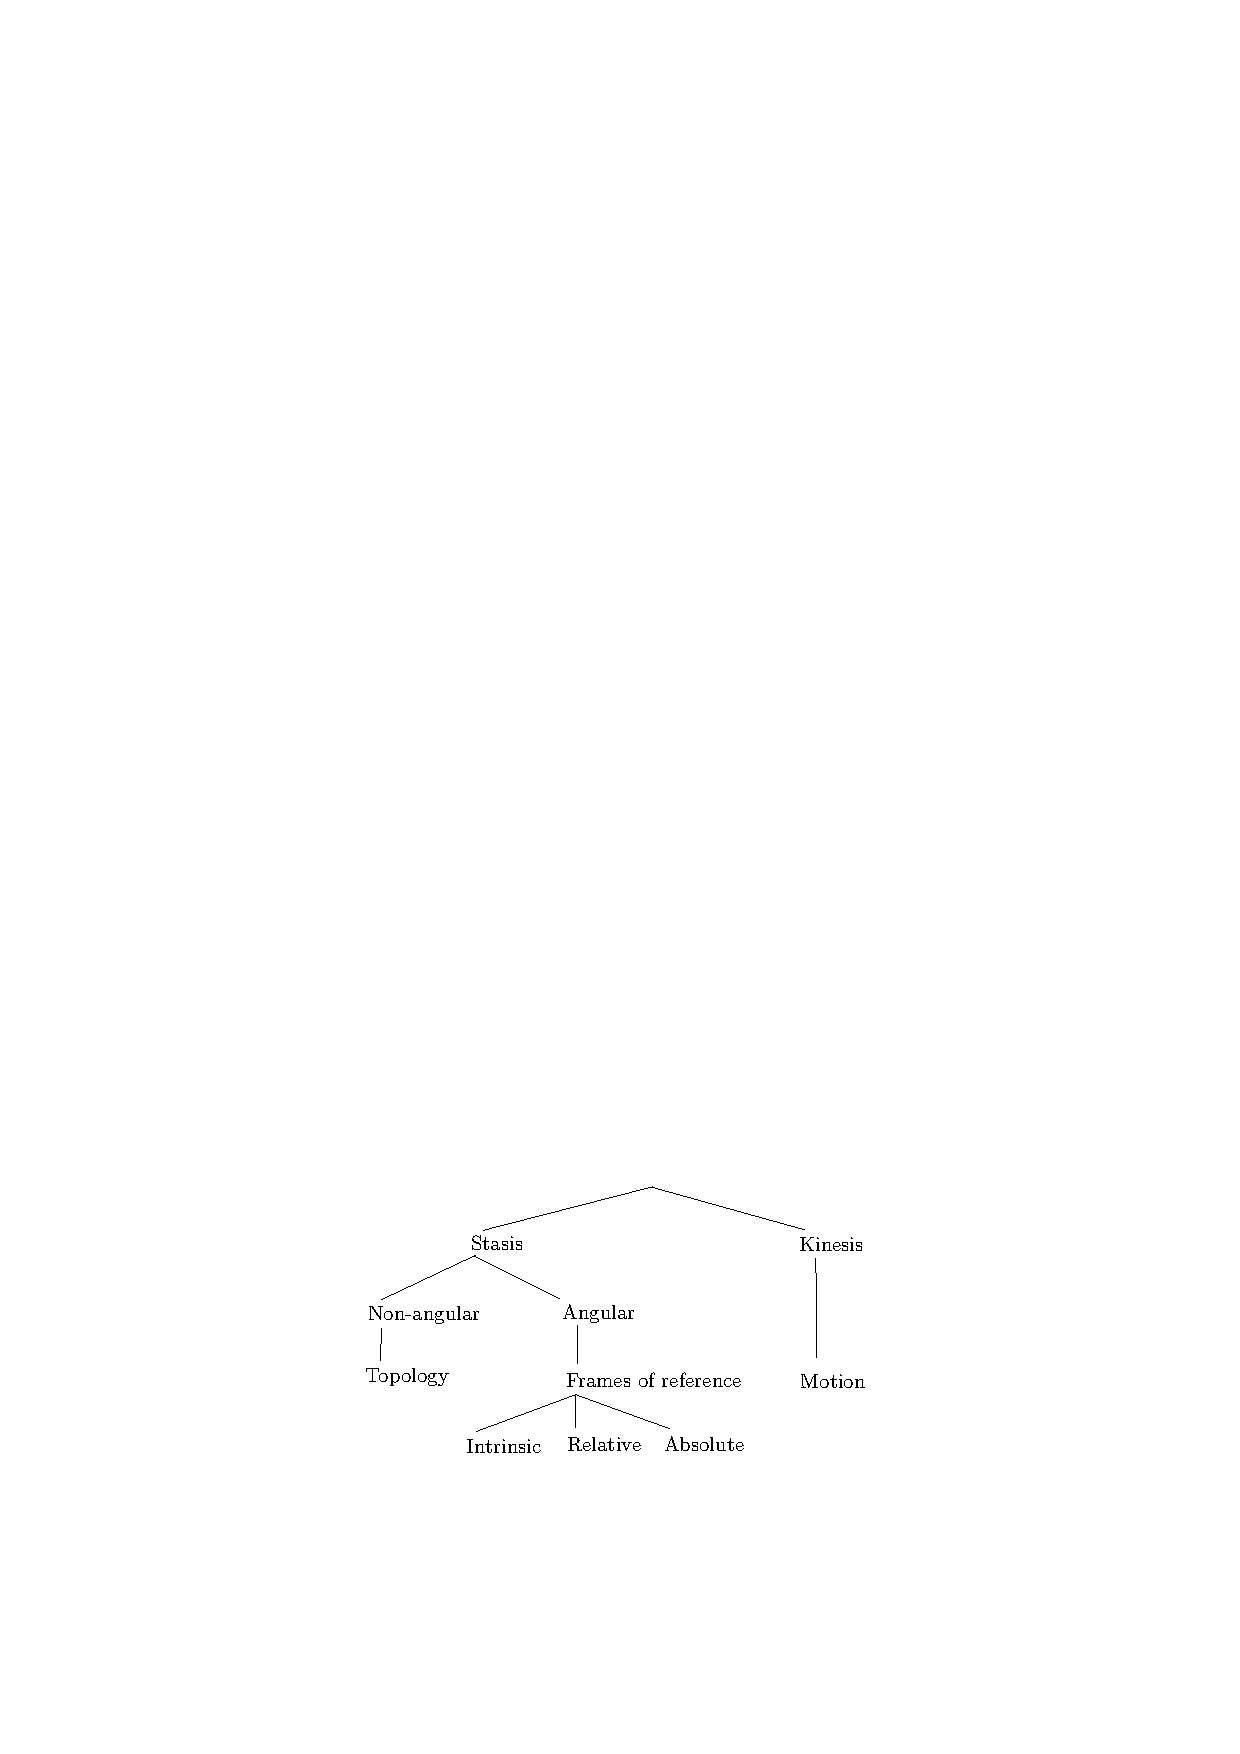
\includegraphics[width=3in]{Graphic/Pictures/Levi-spatial-domain.pdf}
 % Levi-spatial-domain.pdf: 595x842 pixel, 72dpi, 20.99x29.70 cm, bb=0 0 595 842
\caption{Conceptual
subdivisions of statial domain \cite[3]{Levi06}.
\label{fig:Levi-spat-dom}}
\end{figure}


Figure \ref{fig:Levi-spat-dom} displays the partitioning of the spatial domain
found in \cite{Levi06}:  topological description, motion description and frames
of reference are the three sub-domains.  \citeauthor{Levi06} write that the
partition of figure  \ref{fig:Levi-spat-dom} ``does not exhaust the domain (...)
but we have selected these sub-domains because they cover the major themes in
the literature'' and because the selection ``reflects major conceptual cleavages
in the
domain: stasis vs. kinesis on the one hand, and angular vs. non-angular static
descriptions on the other''  \citep[3]{Levi06}.  


In this study,  I  emphasize topological description. The notion of {\it
topological relation markers} (TRM) identifies the terms in a language which
contribute to the description of  topological relations. The aim is thus to
uncover
the core meaning of all  topological relation markers and their semantic
differentiation.

%Topological Tasks: General Introduction
%Sérgio Meira with Steve Levinson, p.28
%sixth volume , field manual



\section{Describing static configurations}
\label{sec:SPA-topo-rel}

In this section, five tasks are presented. They are intended to identify
the topological relation markers  used in  the description of static
configurations. For each task, the methodology and procedure are introduced,
 followed by the results and a brief discussion.
All stimuli  are designed  for investigating topological
relations.  Apart from the one employed in the first task in
section
\ref{sec:SPA-exper1} below,
 the stimuli were  created  by the Language and Cognition Group at the Max
Planck Institute for Psycholinguistics. 


\subsection{Task 1}
\label{sec:SPA-exper1}  


The Sweet-and-Calabash Stimulus  was
designed to pay special attention to the following
variables: (i) the stimuli are real objects, as opposed to pictures (i.e. as
opposed to tasks  2, 3, 4 and 5 of section   \ref{sec:SPA-exper2-3})
and  (ii)  the consultants are school children. The design of the task aimed at
eliciting the linguistic strategies involved
in the general frames of reference, 
 an aspect of the spatial domain which is  difficult (and sometimes
impossible) to
reflect
using picture stimuli.  The reason why school children were
included is that,  since middle-aged  individuals were
going to be the social group involved in subsequent  tasks 
(section \ref{sec:SPA-exper2-3}), the data from
school children may
show  whether their usage of  topological relation markers matches that of 
other social groups.




\subsubsection{Method and procedure}
\label{sec:SPA-exper1-method}

The two objects of the stimulus are a sweet and a container. The sweet is a
peanut paste ball, called {\S kpulikpuli} in both Waali and Chakali, which is
very popular in the region. The container is one hemisphere of a dried hollow
calabash. Both the calabash and the sweet are presented to the consultants
before the experiment. 

The consultants were four teenagers, two girls and two boys. They are divided
into two sex-based groups. Table \ref{tabːSPAsubject-info} displays each
consultant’s identification, sex and section (in Ducie).  All are enrolled in
formal education at Ducie primary school.


\begin{table}[htbp]
\centering
\caption{The sweet and the calabash stimulus: information on consultants 
\label{tabːSPAsubject-info}}
\begin{Itabular}{lllllll}

\Hline
ID & Sexe & Age & Ducie's section  & Order\\
\hline

WISA & m & 11 &  Lobani  & 7,6,5,4,3,2 and 1\\ %& A-w
DAAR & m & 11 & Kuorobani & 7,5,3,1,6,4 and 2\\%& A-d 
MUNE & f & 13 & Kuorobani   & 1,2,3,4,5,6 and 7\\%& B-m
TOMA & f & 12 & Kuorobani    & 2,4,6,1,3,5 and 7\\ %& B-t

\Hline
\end{Itabular}
\end{table}

The task involves two consultants facing each other. They sit on a chair and are
separated by a table on which the sweet and the calabash are placed. One
consultant, B,  is blindfolded. B is requested to ask  {\S kaa a kpulikpuli}
`where is the sweet?'. The other consultant, the information consultant (A),
replies by providing B with the exact location of the sweet.  B must locate the
sweet with one hand. Both consultants are aware of the location of the calabash,
but not that of the sweet.  

Figure \ref{fig:Space-test} illustrates the configuration of the task. The
experiment consists of one session for each consultant, and each session
comprises
seven
situations to be described by  A.  The seven situations are
presented to them in four different orders. The orders 
 are displayed in the last column of table \ref{tabːSPAsubject-info}.    In
figure \ref{fig:Space-test}  the  locations of the sweet, i.e. the seven
possible
situations, are represented as {\it k_{1-7}}:

\begin{itemize}\addtolength{\itemsep}{-0.4\baselineskip}

 \item In {\it k_{1}}  the sweet is inside, covered by the calabash. 
\item In {\it k_{2}} the sweet is inside the calabash, at the bottom.
\item In {\it k_{3}} the sweet is on top of the calabash. 
\item In {\it k_{4}} the sweet is on the right of the calabash for B.
\item In {\it k_{5}} the sweet is on the left of the calabash for B.
\item In {\it  k_{6}} the sweet is in front of B, between B and the
calabash.
\item In {\it k_{7}} the sweet in behind the calabash, between A and the
calabash.
\end{itemize}

\begin{figure}[h!]
 \centering
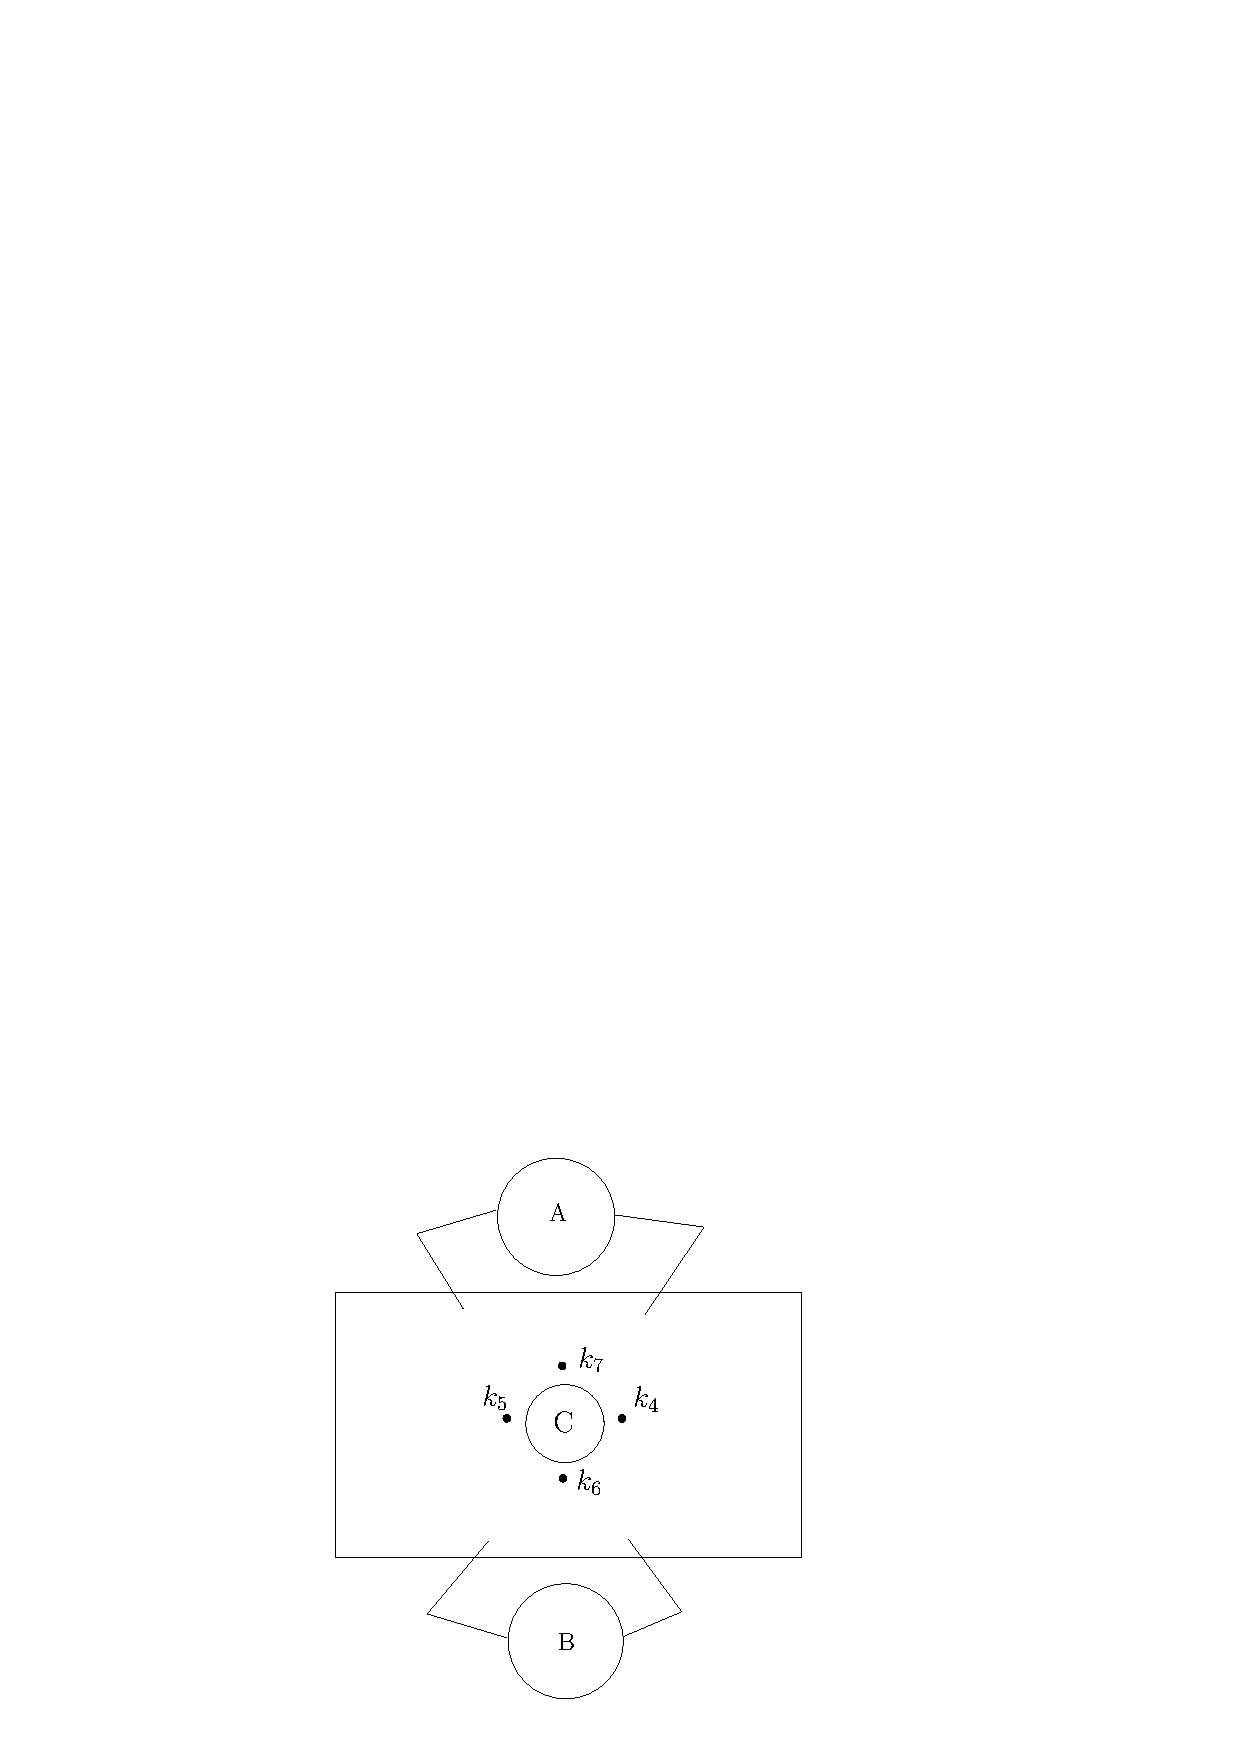
\includegraphics[width=1.8in]{Graphic/Pictures/Settings.pdf}\\
 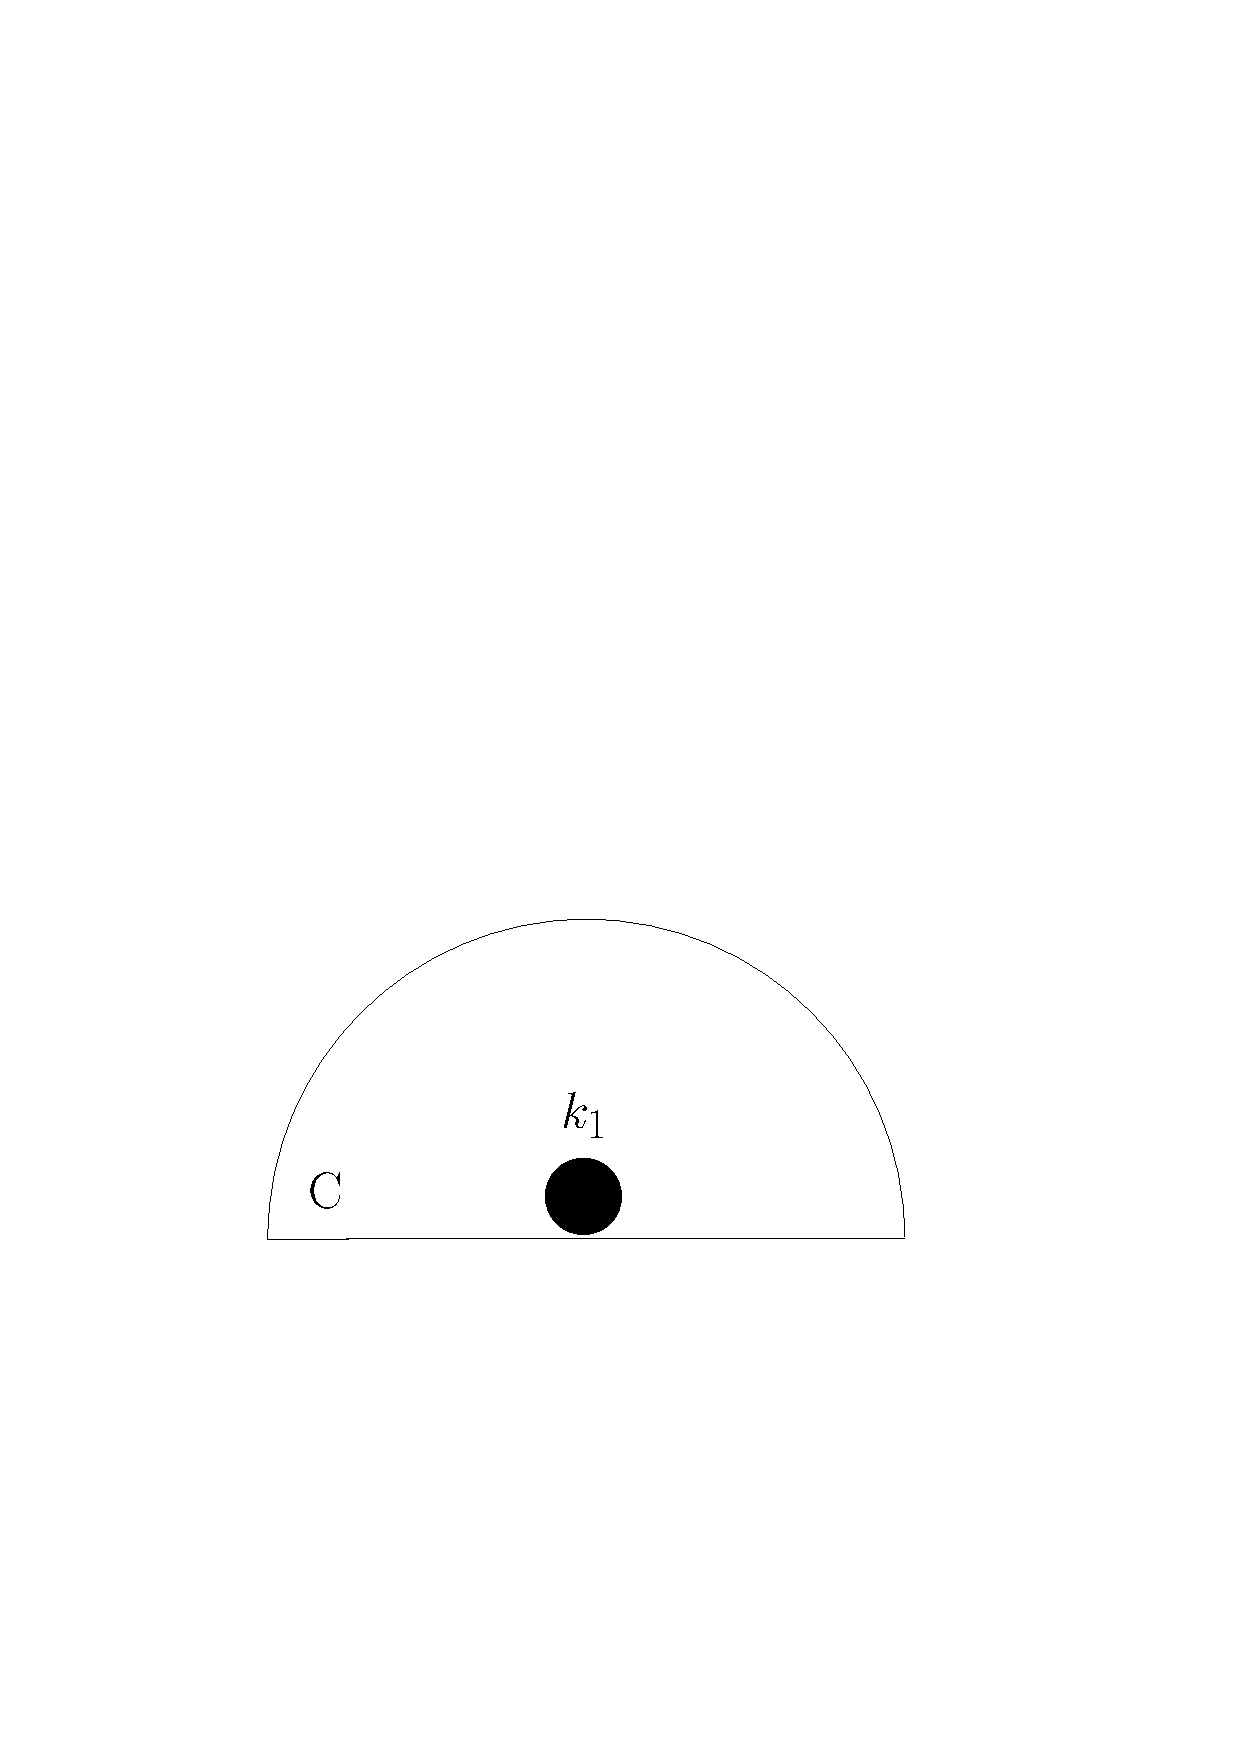
\includegraphics[width=1in]{Graphic/Pictures/K1.pdf}
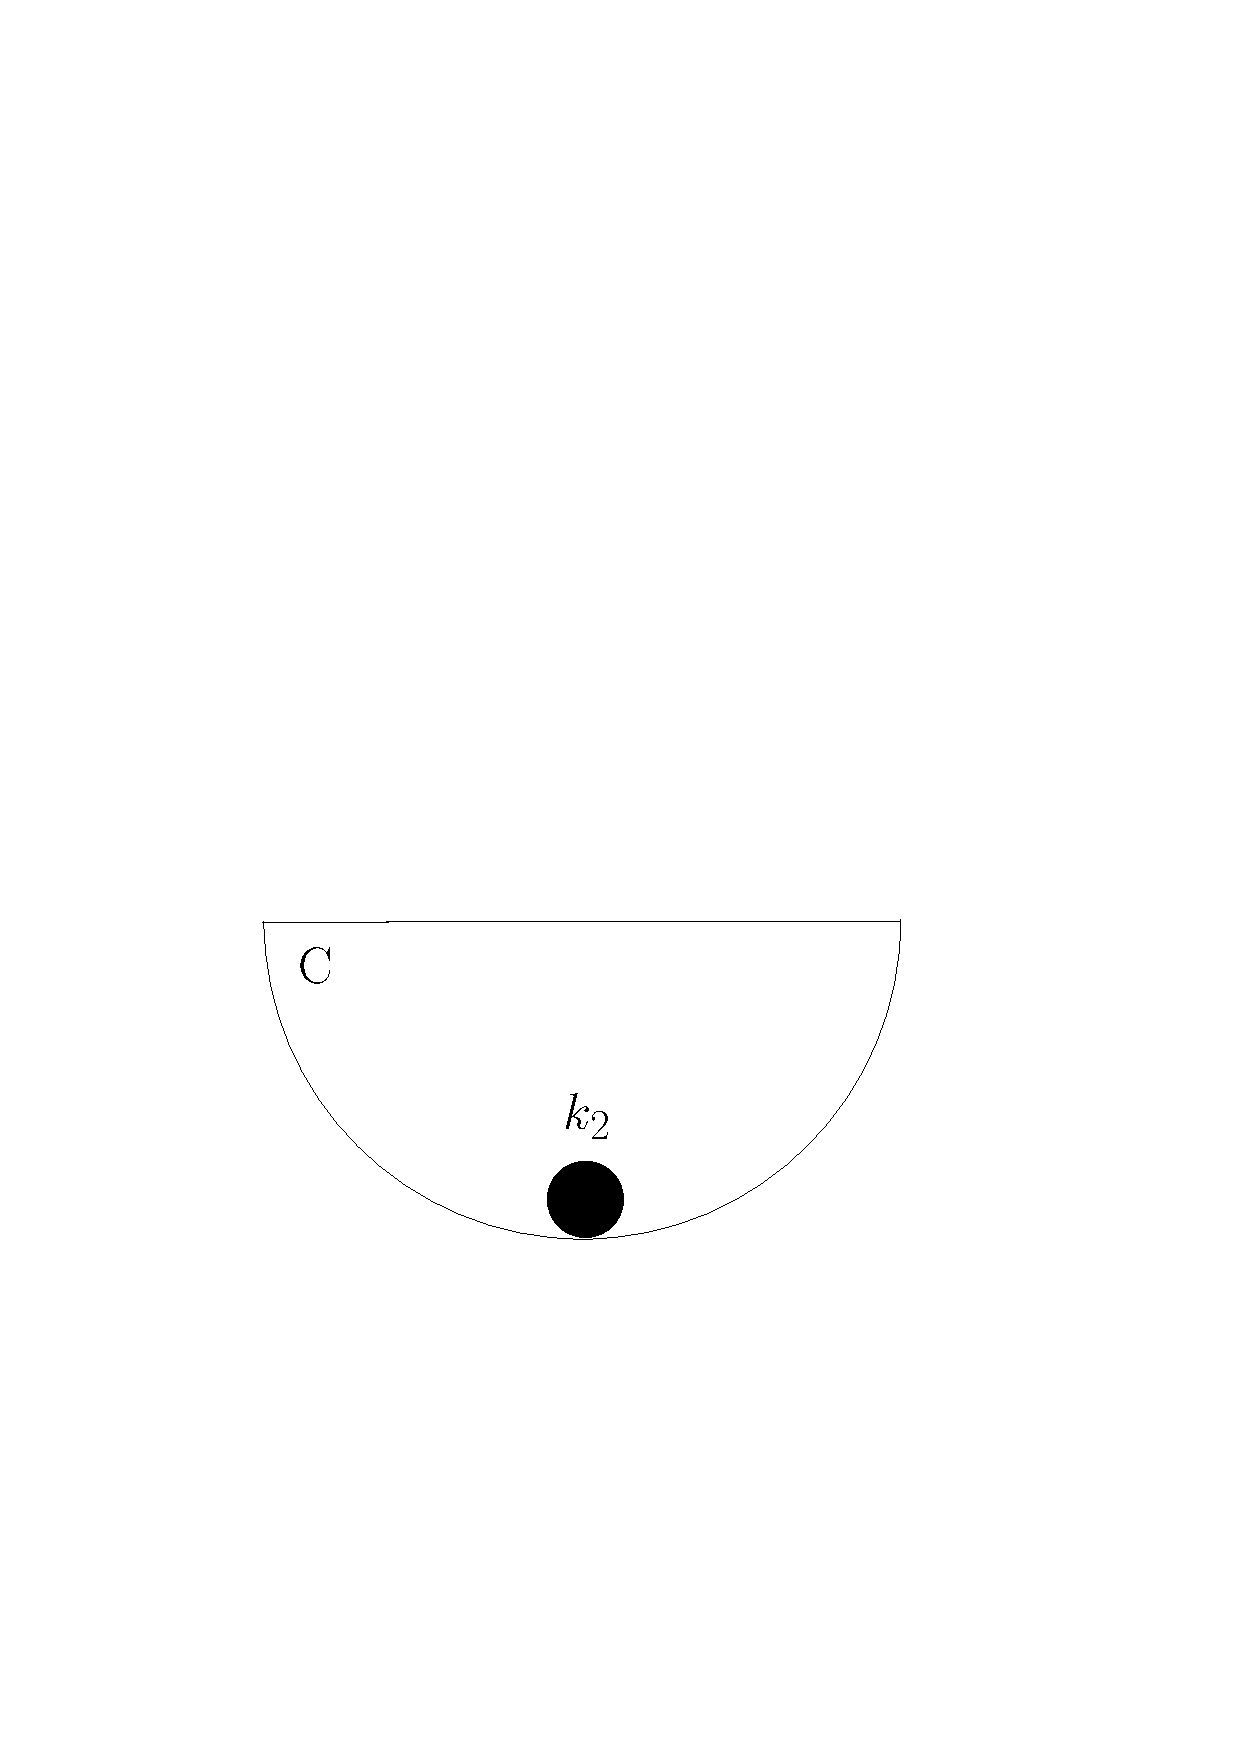
\includegraphics[width=1in]{Graphic/Pictures/K2.pdf}
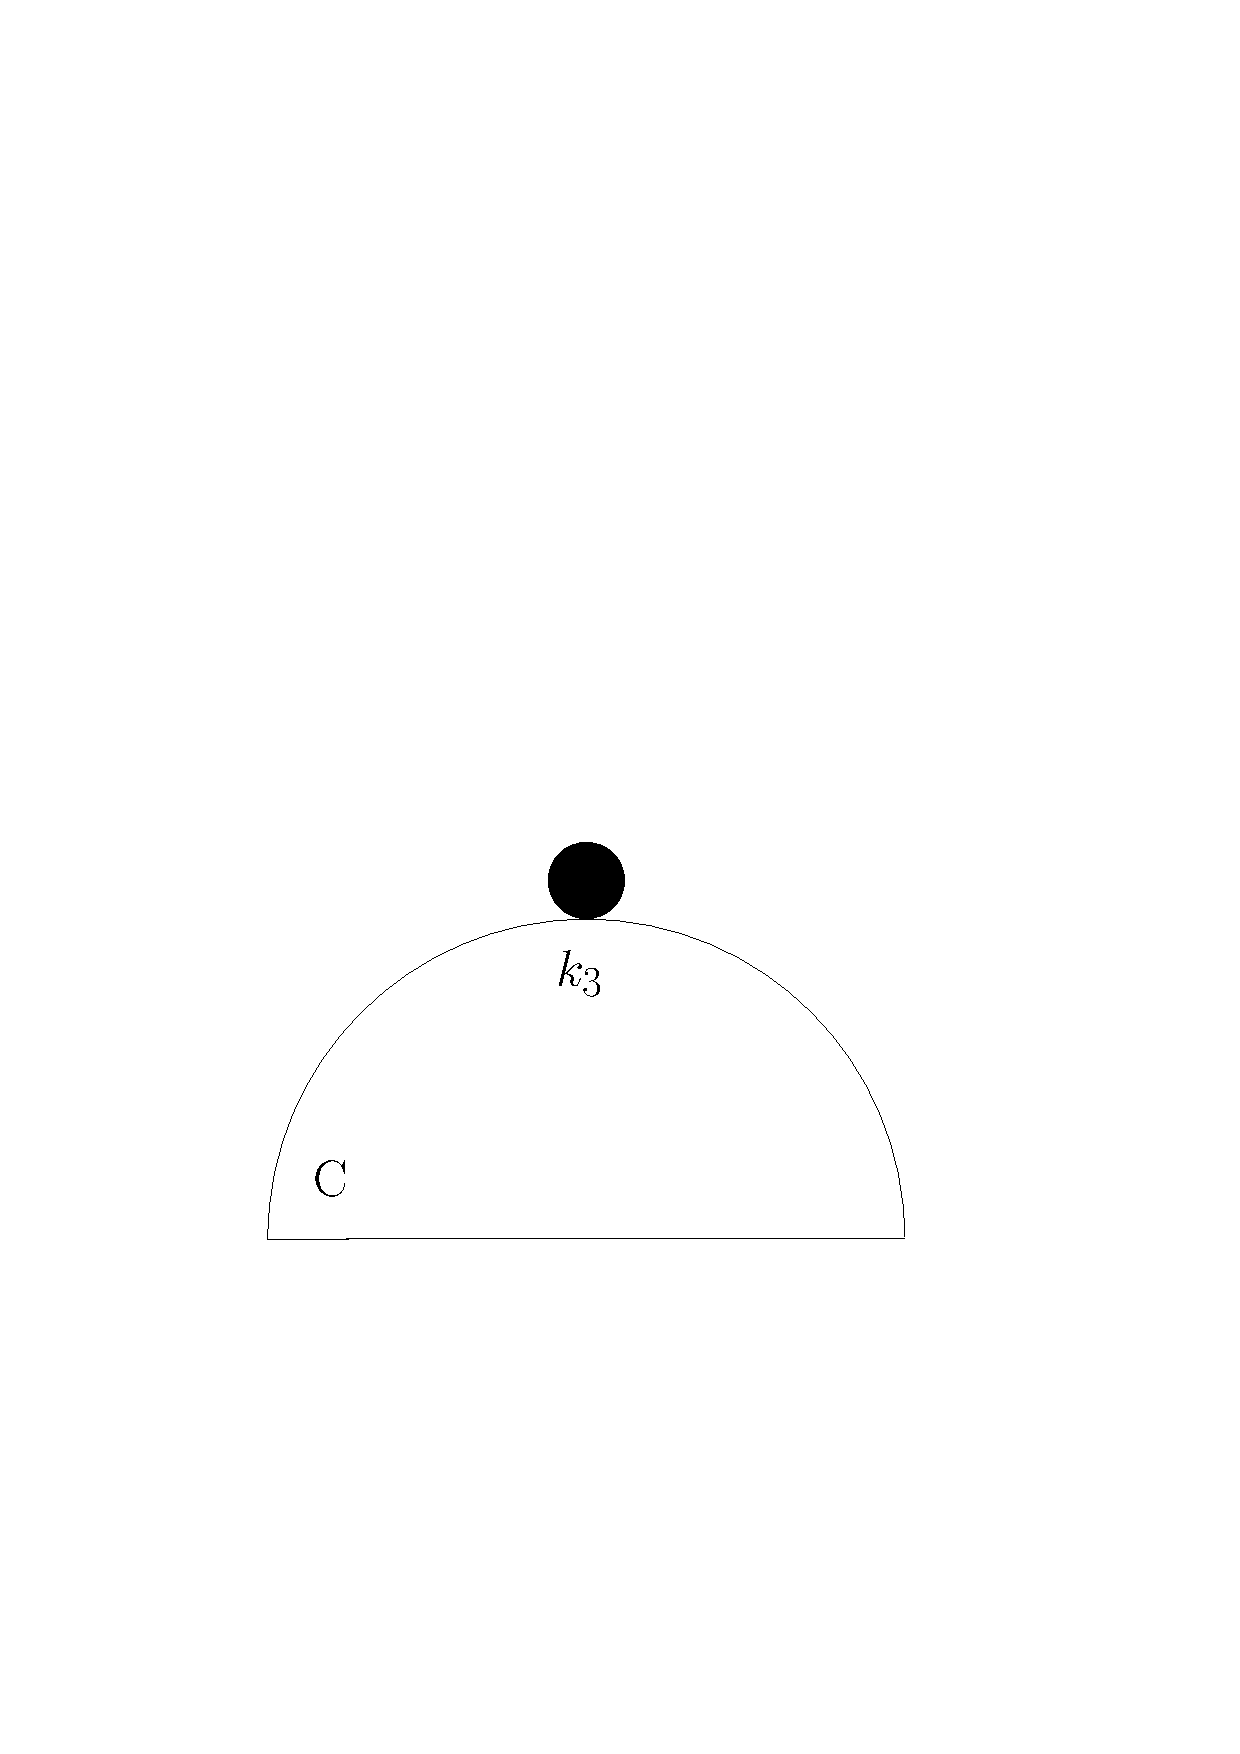
\includegraphics[width=1in]{Graphic/Pictures/K3.pdf}

 % K1.pdf: 2147483647x2147483647 pixel, 0dpi, infxinf cm, bb=
 \caption[Static location test: The sweet and the calabash]{The sweet and the
calabash static location test: A= consultant providing location of kpulikpuli,
B= blindfolded consultant,  C= calabash and k_{1-7}= seven
different locations of kpulikpuli.}
 \label{fig:Space-test}
\end{figure}



The researcher must carefully observe B's behavior. His/her hand must  locate
the sweet at one particular location, and not feel for the calabash or round
about in order to find the sweet.  This is crucial since the instructions given
by A identify seven distinct locations. Failure of B to direct his/her hand
towards one of the seven locations suggests that the instruction was either
misunderstood or ambiguous. Accordingly, the experiment also reveals two aspects
of spatial meaning: (i) the type of frame of reference (i.e. relative, absolute
or intrinsic), and (ii) which strategies  are preferred by A when a situation
can be described with alternative expressions.



\subsubsection{Result and discussion}
\label{sec:SPAresult}

The results are organized and presented according to the seven situations. For
every location,   B formulates  the question as {\S
kaa a kpulikpuli} `Where is the kpulikpuli?'. Then  A
 informs  B  of  the location by providing 
the instructions listed below. In the examples  below, all (a)
sentences are from the language consultant WISA, (b) from DAAR, (c) from MUNE
and (d) from TOMA (see table \ref{tabːSPAsubject-info}).


%Each example provides the four answers given for a particular situation.
%In (\ref{ex:k1}) to (\ref{ex:k7}, the answers (a) are from the subject A-w, (b)
%from A-d, (c) from B-t and (d) from B-m.

%examples (\ref{ex:k1}) to 
%(\ref{ex:k7})   give the


\paragraph{Situation {\it k_{1}}}
\label{sec:SPA-exper1-loca}

The situation {\it  k_{1}}  presents the sweet   inside the calabash, the
calabash facing down, covering the sweet. The expression {\S fala patʃɪgɪɪ}
`inside the calabash' is an ambiguous expression as it can describe either
situation {\it k_{1}} or situation {\it  k_{2}}.  Consequently,  A must provide
a disambiguating phrase. For instance, in (\ref{ex:k1-A-w}) A tells B to open
the calabash, while in (\ref{ex:k1-A-d}) A says that the calabash has been used
to cover the sweet. The verb  {\S dʊa}, functioning here as an existential
predicate denoting a topological relation of coincidence, may be translated as
`be at' and is used throughout.

\begin{exe}
\ex\label{ex:k1}\textit{Situation {\it k_{1}}}\\
 \begin{xlist}
  \ex\label{ex:k1-A-w}
\gll  ʊ dʊa a fala patʃɪgɪɪ nɪ , kpaga lala\\
\textsc{3.sg.wk} be.at \textsc{art} calabash inside \textsc{postp} {} have
open\\
\glt `It is inside the calabash, open it.'

\ex\label{ex:k1-A-d}
\gll  wa dʊa a fala patʃɪgɪɪ nɪ , ba kpajɛ tʃigeu \\
\textsc{3.sg.st} be.at \textsc{art} calabash inside \textsc{postp} {}
\textsc{3.pl.g}b take.\textsc{pfv} cover.\textsc{3.sg}\\

\glt `It is inside the calabash, they took the calabash and  covered it.'


\ex\label{ex:k1-B-t}
 \gll  ʊ dʊa a kɪmpatʃɪgɪɪ nɪ ,  naʊ nɪ , na wa tʃʊa keŋ\\
\textsc{3.sg.wk} be.at \textsc{art} \textsc{thing}.inside \textsc{postp}  {}
see.\textsc{3.sg} \textsc{postp} {} see \textsc{3.sg.st} lie  \textsc{advm}\\
 
\glt `It is inside the thing, see it , see it is lying like that.'


\ex\label{ex:k1-B-m}
\gll  wa dʊa a fala patʃɪgɪɪ nɪ , ba kpajɛ tʃigeu, kpaga a fala lala \\
\textsc{3.sg.st} be.at \textsc{art} calabash inside \textsc{postp} {}
\textsc{3.pl.g}b take.\textsc{pfv} cover.\textsc{3.sg}  have
\textsc{art}
calabash open\\

\glt `It is inside the calabash , they covered it,  open the calabash.'

\end{xlist}
\end{exe}



\paragraph{Situation {\it  k_{2}}}
\label{sec:SPA-exper1-loca}

In {\it k_{2}}   the sweet is inside the  calabash, the calabash facing up.
Situation 
{\it k_{2}} also receives additional information, perhaps to differentiate it
from 
{\it k_{1}}, i.e.  in (\ref{ex:k2-A-d}) `it is open', in  (\ref{ex:k2-A-d})
`look
inside' and in  (\ref{ex:k2-B-m}) `take your hand and enter inside it'.  
As in the situation 
{\it k_{1}}, the  existential predicate  {\S dʊa} is the main verb.

%It may be that the subjects perceive the situation  {\it k_{2}} as more
% canonical than  {\it k_{1}}  when the expression {\S fala patʃɪgɪɪ}  `inside
% the calabash' is used. 


\begin{exe}
\ex\label{ex:k2}\textit{Situation {\it k_{2}}}\\
 \begin{xlist}
  \ex\label{ex:k2-A-w}
\gll  wa dʊa a fala patʃɪgɪɪ nɪ , ʊ patʃɪgɪɪ nɪ \\
\textsc{3.sg.st} be.at \textsc{art} calabash inside \textsc{postp} {}
\textsc{3.sg.poss} inside \textsc{postp} \\

\glt `It is inside the calabash, inside it.'

\ex\label{ex:k2-A-d}
\gll   wa dʊa a fala patʃɪgɪɪ nɪ , ba kpaga lalaʊ\\
\textsc{3.sg.st} be.at \textsc{art} calabash inside \textsc{postp} {}
\textsc{3.pl.g}b have open.\textsc{3.sg}.\\

\glt `It is inside the calabash, it is open.'


\ex\label{ex:k2-B-t}
\gll  ʊ dʊa a fala patʃɪgɪɪ nɪ , a fala patʃɪgɪɪ nɪ , dɪ ɲine ʊ patʃɪgɪɪ nɪ\\
\textsc{3.sg.wk} be.at \textsc{art} calabash inside \textsc{postp} {}
\textsc{art} calabash inside \textsc{postp}  {} \textsc{comp} look   inside
\textsc{postp} \\

\glt `It is inside the calabash, inside the calabash, look inside.'


\ex\label{ex:k2-B-m}
\gll  wa dʊa a fala patʃɪgɪɪ nɪ ,  kpa ɪ neŋ dɪ tʊ̃ʊ̃ a fala patʃɪgɪɪ\\
\textsc{3.sg.st} be.at \textsc{art} calabash inside \textsc{postp} {} take
\textsc{2.sg.poss} hand \textsc{conn} insert \textsc{art} calabash inside\\

\glt `It is inside the calabash,  take you hand and enter the inside
of the calabash.'


 \end{xlist}

\end{exe}



\paragraph{Situation {\it k_{3}}}
\label{sec:SPA-exper1-loca}


In situation {\it k_{3}}, the locative predicate {\S saga} `sit' functions as 
the main verb in all four instructions. It is accompanied by the phrase {\S a
fala ɲuu} `the top of the calabash' which identifies the highest part of
the
calabash with respect to the gravitational axis. The A consultant in
(\ref{ex:k3-A-d}) introduces even more precision by mentioning that the  sweet
is
located  `at the middle of the top of the calabash', i.e. {\S a fala ɲuu bambaaŋ
nɪ}.

\begin{exe}
\ex\label{ex:k3}\textit{Situation {\it k_{3}}}\\
 \begin{xlist}
  \ex\label{ex:k3-A-w}
\gll  wa saga a fala ɲuu nɪ , a fala ɲuu nɪ\\
\textsc{3.sg.st} sit \textsc{art} calabash head \textsc{postp} {}  \textsc{art}
calabash head \textsc{postp}\\

\glt `It sits on the top of the calabash, the top of the calabash.'

\ex\label{ex:k3-A-d}
\gll  wa saga a fala ɲuu bambaaŋ nɪ , ʊ ɲuu\\
\textsc{3.sg.st} sit \textsc{art} calabash head middle \textsc{postp} {}
\textsc{3.sg.poss} head\\

\glt `It sits on the top of the calabash, its top.'


\ex\label{ex:k3-B-t}
\gll  wa saga a fala ɲuu nɪ , ʊ ɲuu nɪ\\
\textsc{3.sg.st} sit \textsc{art} calabash head \textsc{postp} {}
\textsc{3.sg.poss} head \textsc{postp}\\

\glt `It sits on the top of the calabash, its top.'


\ex\label{ex:k3-B-m}
\gll  wa saga a fala ɲuu nɪ\\
\textsc{3.sg.st} sit \textsc{art} calabash head  \textsc{postp}\\

\glt `It sits on the top of the calabash.'

\end{xlist}

\end{exe}




\paragraph{Situation {\it k_{4}}}
\label{sec:SPA-exper1-loca}

A third verb  expresses the spatial relation represented in the situation {\it
k_{4}}. The locative predicate {\S tʃʊa} `lie' functions as the main verb,
except in (\ref{ex:k4-B-t}) where the existential predicate {\S dʊa} is
preferred.  The location of the sweet is on the right of the calabash for B, but
on the left of the calabash for A.  In (\ref{ex:k4}), all the A consultants use
a strategy which projects B's orientation. One way or another, everyone
expresses
the situation as `the sweet lies at {\it your} right hand side'. The 
instructions in (\ref{ex:k4-A-d}) show that pointing at the `side of the
calabash' is inappropriate, unless one can identify one of the two sides. 


\begin{exe}
\ex\label{ex:k4}\textit{Situation {\it k_{4}}}\\
 \begin{xlist}
  \ex\label{ex:k4-A-w}
\gll  wa tʃʊa ɪ nendul nɪ , ɪ nendul nɪ\\
\textsc{3.sg.st} lie \textsc{2.sg.poss} hand.right \textsc{postp} {}
\textsc{2.sg.poss} hand.right \textsc{postp} \\

\glt `It is on your right hand side, you right hand side.'

\ex\label{ex:k4-A-d}
\gll  wa tʃʊa a fala logun nɪ , ɪ nendul nɪ\\
\textsc{3.sg.st} lie \textsc{art} calabash side  \textsc{postp}  {}
\textsc{2.sg.poss} hand.right \textsc{postp}\\

\glt `It is on the side of the calabash, your right hand side.'

\ex\label{ex:k4-B-t}
\gll  wa dʊa ɪ nendul nɪ keŋ\\
\textsc{3.sg.st} be.at \textsc{2.sg.poss} hand.right \textsc{postp}
\textsc{advm}\\
\glt `It is on your right hand side like that.'


\ex\label{ex:k4-B-m}
\gll  wa tʃʊa ɪ nendul nɪ , a fala logun nɪ , ai dɪ waa a fala logun \\
\textsc{3.sg.st} lie \textsc{2.sg.poss} hand.right \textsc{postp} {}
\textsc{art}
calabash side  \textsc{postp}  {} no  \textsc{comp} come \textsc{art} calabash
side\\
\glt `It is on your right hand side, on the side of the calabash, no! come to
the side of the calabash.'

 \end{xlist}

\end{exe}



\paragraph{Situation {\it k_{5}}}
\label{sec:SPA-exper1-loca}

Situation {\it k_{5}} portrays the reverse of situation {\it k_{4}}, that is,
the sweet is on the left of the calabash for B.  I anticipated that the 
locative  predicate {\S tʃʊa} `lie'  would function similarly as it does for
situation   {\it k_{4}}.  As expected,  the instructions are alike in both the 
situations  {\it k_{4}} and  {\it k_{5}},  except that instead of {\S ɪ nendul}
`your right hand'  we get {\S ɪ neŋgal} `your left hand'. The expression {\S a
fala muŋ} `under the calabash' is
understood in this case as referring to the base or the bottom of the
calabash, and not an 
area underneath it. 



\begin{exe}
\ex\label{ex:k5}\textit{Situation {\it k_{5}}}\\
 \begin{xlist}
  \ex\label{ex:k5-A-w}
\gll  wa tʃʊa ɪ neŋgal nɪ , ɪ neŋgal nɪ\\
\textsc{3.sg.st} lie \textsc{2.sg.poss} hand.left \textsc{postp} {}
\textsc{2.sg.poss} hand.left \textsc{postp}\\
\glt `It is on your left hand side, your left hand side.'

\ex\label{ex:k5-A-d}
\gll  wa tʃʊa a fala logun nɪ , ɪ neŋgal nɪ\\
\textsc{3.sg.st} lie \textsc{art} calabash side  \textsc{postp} {}
\textsc{2.sg.poss} hand.left \textsc{postp}\\
\glt `It is on the side of the calabash, your left hand side.'

\ex\label{ex:k5-B-t}

\gll wa dʊa ɪ neŋgal nɪ keŋ , ɪ neŋgal nɪ , dɪ waa a fala pe banɪ tɪŋ \\
\textsc{3.sg.st} be.at \textsc{2.sg.poss} hand.left \textsc{postp} \textsc{adv} 
{}   \textsc{2.sg.poss} hand.left \textsc{postp} {} \textsc{comp} come
\textsc{art} calabash end  place \textsc{art}\\
 
\glt `It is on your left like this, your left, come towards the calabash's 
place.'

\ex\label{ex:k5-B-m}
\gll  wa tʃʊa ɪ neŋgal nɪ , a fala muŋ nɪ\\
\textsc{3.sg.st} lie \textsc{2.sg.poss} hand.left \textsc{postp} {} \textsc{art}
calabash base \textsc{postp}\\
\glt `It is on your right hand side, at the base of the calabash.'
 \end{xlist}

\end{exe}



\paragraph{Situation {\it k_{6}}}
\label{sec:SPA-exper1-loca}

In situation {\it k_{6}} the sweet is between  B and the calabash. Every
A portrays the sweet as being  at  {\S ɪ sʊʊ} `your front', i.e
in front  of  B. In (\ref{ex:k6-A-d}),   A adds that the
sweet is in front of the calabash, which is the other option to project
B's
orientation. Except for (\ref{ex:k6-B-t}), the instructions are built with the
locative  predicate {\S tʃʊa} `lie'.

 


\begin{exe}
\ex\label{ex:k6}\textit{Situation {\it k_{6}}}\\
 \begin{xlist}
  \ex\label{ex:k6-A-w}
\gll wa tʃʊa ɪ sʊʊ  nɪ keŋ , ɪ sʊʊ nɪ\\
\textsc{3.sg.st} lie \textsc{2.sg.poss} front \textsc{postp} \textsc{adv} {} 
\textsc{2.sg.poss} front \textsc{postp}\\

\glt `It is in front of you.'

\ex\label{ex:k6-A-d}
\gll wa tʃʊa ɪ sʊʊ  nɪ , a fala sʊʊ  nɪ \\
\textsc{3.sg.st} lie  \textsc{2.sg.poss} front \textsc{postp}   {} \textsc{art}
calabash front \textsc{postp}\\ 

\glt `It is in front of you, in front of the calabash.'


\ex\label{ex:k6-B-t}
\gll wa dʊa ɪ sʊʊ nɪ \\
\textsc{3.sg.st}  be.at  \textsc{2.sg.poss} front \textsc{postp} \\

\glt `It is in front of you.'

\ex\label{ex:k6-B-m}
\gll wa tʃʊa ɪ sʊʊ  nɪ\\
\textsc{3.sg.st} lie \textsc{2.sg.poss} front \textsc{postp} \\

\glt `It is in front of you.'


 \end{xlist}

\end{exe}



\paragraph{Situation {\it k_{7}}}
\label{sec:SPA-exper1-loca}

In situation {\it k_{7}}, the sweet is located between  A and the
calabash. Both the  verbs {\S tʃʊa} and {\S dʊa} are used. The phrase {\S a fala
gantal} `the back of the  calabash' is found in
(\ref{ex:k7-A-w}) and (\ref{ex:k7-B-t}) to
describe the  {\it k_{7}} location relative to B, whereas the phrase
{\S n̩ sʊʊ}, occurring in (\ref{ex:k7-A-d}) and (\ref{ex:k7-B-m}), accounts
for 
situation {\it k_{7}} relative to A.  As for situation {\it k_{5}}, the
expression {\S a fala muŋ}  in (\ref{ex:k7-B-m})  is
understood as  `the base of the calabash'. 




\begin{exe}
\ex\label{ex:k7}\textit{Situation {\it k_{7}}}\\
 \begin{xlist}
  

\ex\label{ex:k7-A-w}
\gll wa tʃʊa a fala gantal nɪ , a fala gantal nɪ \\
\textsc{3.sg.st} lie \textsc{art} calabash back \textsc{postp} {}  \textsc{art}
calabash back  \textsc{postp}\\
\glt `It is behind the calabash.'

\ex\label{ex:k7-A-d}
\gll wa dʊa a fala gantal nɪ , n̩ sʊʊ nɪ, ʊ gantal nɪ\\
\textsc{3.sg.st} be.at \textsc{art} calabash back \textsc{postp} {}
\textsc{1.sg.poss} front \textsc{postp}  \textsc{3.sg.poss} back \textsc{postp}
\\
\glt `It is behind the calabash, in front of me, at its back.'

\ex\label{ex:k7-B-t}


\gll wa dʊa n̩ sʊʊ nɪ keŋ , a fala gantal nɪ\\
\textsc{3.sg.st}  be.at \textsc{1.sg.poss} front \textsc{postp} \textsc{adv} {} 
\textsc{art} calabash back  \textsc{postp} \\
\glt `It is in front of me like that, behind the calabash.'


\ex\label{ex:k7-B-m}
\gll wa tʃʊa n̩ sʊʊ nɪ keŋ , a fala muŋ nɪ\\
\textsc{3.sg.st} lie \textsc{1.sg.poss} front \textsc{postp} \textsc{adv} {}
\textsc{art} calabash  base \textsc{postp}\\
\glt  `It is in front of me like that,  at the base of the calabash.'

 \end{xlist}

\end{exe}



\subsubsection{Summary}
\label{sec:SPA-exper1-sum}

In the sentences used by the A consultants, the sweet  is always associated with
the
figure, which occupies the grammatical subject slot, and 
is referred to by using the strong pronoun {\S wa} to a greater extent than the
weak pronoun {\S ʊ}.   The spatial expressions are constructed
using the three following topological
relation markers. First,  a postposition {\S nɪ} is present in
all the utterances.  It is the only general locative postposition in the
sentences and it  only indicates that there is a locative relation. Secondly,  a
main verb consisting of the general existential predicate {\S dʊa}
`be at',  or  the locative predicates  {\S tʃʊa} `lie' or {\S saga} `sit',  sets
up a relation of localization of the figure with respect to the ground. The
third 
topological
relation marker is a phrase of the type {\S a fala X} `the
calabash X',  of
which X is a
position where the meaning of the word  filling it
localizes the figure to a search domain. In that position, the words {\S
patʃɪgɪɪ, ɲuu,
logun, nendul, neŋgal, sʊʊ, muŋ} and {\S gantal} describe a specific spatial
relation of the figure with respect to the ground. All of them are lexical
items which otherwise refer to (human) body parts. These characteristics are
displayed in (\ref{ex:sum-task-1}).

\begin{exe}
\ex\label{ex:sum-task-1}
 
 \Tree{ & \Kq{S}\Bq{dl}\Bq{dr} &&&\\
\Kq{\it n} && \Kq{VP}\Bq{dl}\Bq{dr}&&\\
 & \Kq{\it v}  &&\Kq{PP}\Bq{dl}\Bq{dr} &\\
&& \Kq{NP}\Bq{dl}\Bq{dr} && \Kq{\it postp}\\
& \Kq{\it n}&  &\Kq{\it n} &} 

\glll {{[ ]}_{\sc subj}}  {{[ ]}_{pred}}  {{[ ]}_{obl}} \\
{\sc figure}  {\sc localisation}  {{\sc localisation}+{\sc ground}}\\
{\it n} {\it v}     {{\it n}   {\it n}  {\it postp}} \\
\glt

\end{exe} 



By and large,  A orients B with a relative exocentric (or
altercentric) frame of reference, i.e.  a frame which involves
 mental rotations to make the locations fit B's egocentric frame of reference.
This frame of reference projects the deictic center onto the
addressee (i.e. B) and the situation is seen  from the perspective of
the addressee. This strategy is used to locate the sweet in situations  {\it
k_{4-7}}.
Still, a relative egocentric frame of reference is used by three consultants for
situation {\it k_{7}}.  A reference to an intrinsic frame of reference is
observed in situation {\it k_{3}} where the sweet is described as being  `at the
head of' the calabash, i.e. on top of it. If the notion of containment is
seen as an inherent
part of the calabash, situations  {\it k_{1}} and {\it k_{2}} may also be
treated as involving a reference to an intrinsic frame of reference. The
absolute
frame of reference was not used to locate the sweet.
 


\subsection{Tasks 2, 3, 4 and 5}
\label{sec:SPA-exper2-3}


The four remaining tasks are introduced under  the same heading since they
necessitate  similar methods and  procedures which involve  ``the collection of
data directly in the field using standardized stimuli that cover a shared
extensional grid, allowing close and accurate comparisons of semantic
distinctions'' \citep[860]{Amek07b}.    The stimuli used are all designed by the
Language and Cognition Group of the Max Planck Institute for Psycholinguistics
in Nijmegen.\footnote{I am grateful to the Language and Cognition Group, Max
Planck Institute for
Psycholinguistics in Nijmegen for allowing me to use  
their material and to reproduce the illustrations. The reproductions are found
in
 figure \ref{fig:TRPS-1-24} to figure  \ref{fig:CPS-35-41}.} The four stimuli
consist of
pictures and illustrations
depicting static locative scenes. These elicitation tools improve  on the
stimulus presented in
section \ref{sec:SPA-exper1} by depicting a wider range of situations. 



%\subsubsection{Method and procedure}
%\label{sec:SPA-exper1-method}

\subsubsection{Method and procedure}
\label{sec:SPA-exper2-method}

The method and procedure are similar to those described in section
\ref{sec:SPA-exper1-method}. The data to be analyzed correspond to the answers
to the question ``where is X?'',   that is,  a question seeking information
about the location of a figure with respect to a ground. For instance, to an
illustration which depicts a cup  on a table (see  illustration 1 of the
Topological Relations Picture Series (TRPS) in figure \ref{fig:TRPS-1-24}),  if
one is interested in how to express  the spatial relation of the cup with
respect to the table, then one asks `where is the cup'.\footnote{See 
\cite{Levi03b} and 
\citet[553-562]{Levi06} to appreciate the outcome of this
method of
elicitation.}  The descriptions of the stimuli provide the necessary material to
identify recurrent linguistic patterns.  Authors and  practitioners of the
stimuli recommend that the tasks should be conducted with at least three 
individuals.  Four individuals conducted the experiments,  one male and one
female from Ducie and one male and female from Gurumbele. Let us now consider
the
details of each  stimulus.



The second stimulus, the Topological Relations
Picture Series
(TRPS) \citep{Bowe93},  is a set of
71  illustrations depicting various locative
relations. This stimulus was originally
designed by Melissa Bowerman and has been used to elicit data from a wide range
of languages \cite[see][7-9]{Levi06}. Because  the pictures depict a variety of
topological notions,  the result of the elicitation provides us with a diverse
set of spatial expressions. The illustrations are reproduced in figures
\ref{fig:TRPS-1-24} to \ref{fig:TRPS-49-71}.

The stimulus for the third task is the  Picture Series for Positional
Verbs (PSPV)  \citep{Amek99}. It consists of 68  pictures in which nine
different
figure objects (stick, ribbon, cloth, rope, cassava, bottle, ball, beans, pot)
are  placed in relation to seven different grounds (table, tree branch, tree
stump, tree trunk, basket, rock, earth)  in various positions (canonical vs.
non canonical) \citep[861]{Amek07b}.\footnote{\cite{Amek07b} is a selection of
articles  on typologically varied languages  
gathered in a special issue
of the journal {\it Linguistics} edited by Ameka and Levinson. The author of
each
article used the  Picture Series for Positional Verbs. } As its name suggests,
the PSPV is more
oriented towards producing finer distinctions in the verbal component of
locative statements. The pictures are given in figures \ref{fig:PSPV-1-24} to
\ref{fig:PSPV-49-68}.


% Ameka, Felix; De Witte, Carlien; and Wilkins, David (1999). Picture series
%for
% positional
%  verbs: eliciting the verbal component in locative descriptions. In Field
%Manual % 1999, David
%  Wilkins (ed.), 48–56. Nijmegen: Max Planck Institute for Psycholinguistics.


The last two stimuli  are used specifically for the description of  three
subdomains: containment, support, and adhesion/attachment.  The fourth
stimulus,  the Containment Picture Series (CPS) \citep{Meir01a},  explores
further the
notion of
containment. It consists of 41 pictures representing configurations such as
``full
and partial containment, containment in a fluid and granular medium,
containment in matter and hollow space, and  `functional’ and `geometrical’
containment are depicted''  \citep[33]{Meir01a}. Finally, the fifth stimulus,
the
Support  Picture Series (SPS)  \citep{Meir01b},  consists
of  47  scenes specifically targeting  the notions of contact, support,
adhesion, and attachment. Both the CPS amd SPS are reproduced in figures 
\ref{fig:Support-1-20} 
to \ref{fig:CPS-35-41}.

%Need reference... for CPS and SPS

\subsubsection{Result and discussion}
\label{SPA-exper2-res-discuss}

In general a picture-naming situation  is described with at least one
full clause. The consultants answer  the question {\S kaa X?} `where is X', X
 usually designates the figure in the answer.  When the tasks were
carried out, this 
question  was preferred to the equivalent {\S lie nɪ dʊa X?} `where is X', 
which was believed to  prime the existential predicate {\S dʊa}
`be at'. 


%correction

An investigator using  these stimuli is warned  that  they are not
``intended to be a mechanical elicitation procedure- the investigator may need
to choose alternative local items to be found in similar configurations
(...)'' \cite[9]{Levi06}. In fact, my four consultants, whom I thought might
have  least difficulty with the stimulus, found themselves unable to answer
on some occasions because  they were unfamiliar with the items depicted, e.g.
rotary dial telephone  (TRPS 25), kennel (TRPS 6, 71), light bulb and lamp
(TRPS 7, 13, 52, 63), aquarium (TRPS 32), (sail-) boat (TRPS 11, CPS 20), stamp
(TRPS 3,
28), window glass (TRPS 48), antenna (CPS 30), island (CPS 41), leaf in the
nose (SPS 15), wedge jammed in hole on tree stump (SPS 47) and cabinet door
(TRPS 61).  Other pictures were
found hard to interpret since the relation, the figure or the ground were
perceived as unclear.  To overcome confusion I had to assign other
items to those depicted, for example the boat  became a log  in
situation TRPS  11.   


The resulting dataset consists of more than 900  utterances (i.e.
four
individuals and 227  pictures)  for the TRPS, PSPV, CPS and  SPS
stimuli. Although on a few occasions the consultants hesitated,
restarted or changed a response, I tried to  get  at least one utterance per
consultant for each situation. Alternative answers were recorded as well.



Generally, the utterances show similarities with those of task 1  (see summary
in section \ref{sec:SPA-exper1-sum}). Correspondingly, the basic means of
expressing static location are the following: (i) the postposition {\S nɪ}, 
which is present in almost all the utterances, (ii) a single verb, which is
either the general existential predicate {\S dʊa} `be at',  or one of a series
of locative predicates, and (iii) a relational nominal predicate following the
ground-object. 


\section{Topological relations}
\label{sec:SPA-tr}

This section introduces the basic locative construction (section
\ref{sec:SPA-blc}) and the topological relation markers (section
\ref{sec:SPA-trm}). The discussion is based on the answers provided by four
consultants on the four tasks presented in section \ref{sec:SPA-exper2-3}.


\subsection{Basic locative construction}
\label{sec:SPA-blc}

The {\it basic locative
construction} (BLC) of a language is  the prototypical  and predominant
construction used to locate a figure with respect to a ground \cite[15]{Levi06}.
In this section the responses given for the four stimuli presented in section
\ref{sec:SPA-exper2-3}  are organised
into three:
first, I introduce the BLC in Chakali, then I identify the modulated
construction, i.e those which do not conform exactly to the prototypical BLC,
and finally  I present the non-basic locative
constructions used to describe the scenes depicted in the stimuli.


The majority of the  sentences in the dataset resemble the construction given in
(\ref{ex:PSPV4}), although some sentences appear with the focus particle
following the postposition {\S nɪ}. The
focus particle is a pragmatic marker which identifies for the hearer the topical
subject (i.e. may be distinct from the grammatical subject) and does not convey
locative meaning. The focus particle will be ignored in the discussion. 
The second line  in (\ref{ex:PSPV4}) associates parts of the sentence with a
`conceptual level'. On
that line one can find notions such as figure and ground (see section
\ref{sec:SPA-back-mot}) and \textsc{trm}, which stands for {\it topological
relation marker}. These are the linguistic expressions which convey  the 
spatial
relationships in Chakali. The third line makes a correspondence between the
utterance-level and the grammatical relation-level. The figure {\S a gar} `the
 cloth'  functions as subject ({\sc subj}) and the phrase {\S a tabul ɲuu nɪ}
`on the table' functions as oblique object  ({\sc obl}) of the main
predicate  ({\sc pred}). The last line is a free translation which captures  the
general meaning of the situation. It is accompanied by a reference to the
illustration which the first line describes.



\begin{exe}
\ex\label{ex:PSPV4}
\glll {[à gár]} {[ságá]} {[à tábùl ɲúù nɪ̀]}\\
\textsc{figure} \textsc{trm} {\textsc{ground}+\textsc{trm}}\\
 \textsc{subj}   \textsc{pred} \textsc{obl}\\
\glt `The cloth is on the table.' (PSPV 4)
\end{exe}


In (\ref{ex:PSPV4}), the spatial relation is expressed via three topological
relation markers, that is,  the main predicate {\S saga} `be on' or `sit', the
postposition  {\S nɪ} and the relational nominal predicate {\S ɲuu} `top of'.
The main predicate  {\S saga}  denotes a stative event which  localizes the
figure with respect to the ground.  The postposition  {\S nɪ} has no other
function than to signal that the oblique object is a locative phrase. The
relational nominal predicate {\S ɲuu} designates the search domain and depends
on the reference entity of the ground (i.e. {\S tabul}). The three topological
relation markers are discussed in more detail in section \ref{sec:SPA-trm}.



 %Each may or may not be associated with a
%specific  conceptual component of locative expression. (pos verb vs. ni)

%Chakali as a single locative verb languages 

%The site/ describe a specific  spatial relation with respect to the ground,
%localize the figure in relation to a particular search domain

%Oblique arguments, however, can simply be omitted without any grammatical
%adjustment.


\subsubsection{Alternations of the BLC}
\label{sec:SPA-modulatedBLC}

In this section,   the  recurrent patterns which affect to a certain extent the
BLC are shown. As stated earlier, the prototypical BLC in Chakali is a single
verb construction. However,  the examples in (\ref{ex:two-verb-blc}) show  that
a succession of two verbs is possible. The   two adjacent verbs function as main
predicate and a  single event is expressed.

\begin{exe}
\ex\label{ex:two-verb-blc}{\it Two-verb BLC}
\begin{xlist}

\ex\label{ex:SPS-29}
\gll baal tʃara saŋa daanãã nɪ \\
man straddle sit branch {\postp}\\
\glt `A man straddle on a tree branch.' (SPS-29)

\ex\label{ex:TRPS30b}
\gll  ŋmɛŋ guti saga kʊzaa nʊã nɪ\\
 rope coil be.on basket mouth  {\postp}\\
\glt `A rope lies coiled on a basket.' (PSPV 19)


\ex\label{ex:CPS-06}
\gll  daanɔ̃n tʃʊa dʊgʊlɪ a fala nɪ\\
fruit lie near {\art} calabash {\postp} \\
\glt `A fruit lies near the calabash.' (CPS 06)


\end{xlist}
\end{exe}

Other instances which
diverge from the prototypical BLC are those lacking the postposition {\S nɪ}.
These cases occur only with the verb {\S tɔ} `cover', {\S tʃawa}
`hold' and {\S go/goro} `circle'. 
There is an example of each in (\ref{ex:SPA-abs-postp}).

%go = enclose but not contained

\begin{exe}
\ex\label{ex:SPA-abs-postp}{\it Absent postposition}
\begin{xlist}

% \gll a gar tɔ a teebul ɲuu ro \\
%  {\art} cloth cover {\art} table {\reln .top} {\foc} \\
% \glt `The cloth covers the top of the table' (TRPS 29)
% 
\ex\label{ex:SPA-TRPS-62}
 \gll daa tɔ kɔlbaanʊã\\
 wood cover bottle.mouth\\
 \glt `A wood covers the bottle's mouth.' (TRPS 62)

\ex\label{ex:SPA-SPS-18}
\gll garzagatii tʃawa ɲupʊna \\
rag hold hair\\
\glt `A hairband holds hair.' (SPS 18)

\ex\label{ex:SPA-SPS-18}
\gll  a ŋmɛŋ go a daa ra  \\
 {\art} rope circle  {\art} tree {\foc}\\
\glt `The rope is around the tree.' (TRPS 55)
\end{xlist}
\end{exe}

% Notice that the illustrations
% SPS-29 and SPS-31 contrast with SPS-30 and SPS-32 such that they all involve a
% man sittting on a branch or a wall, yet straddling is depicted only on SPS-29
% and SPS-31. Since the illustrations were presented in their numerical order,
% the need for the consultant to appeal to further precision may explain the
%usage
% of two verbs.  Two consultants used {\S tʃara saŋa} and  {\S guti saga}, the
%other
% two used exclusively {\S saŋa} and {\S  saga}.

Some scenes are perceived with more than  one figure and 
one ground. Examples (\ref{ex:SPA-two-obl}) show that  two oblique phrases may
be used when  one wants to mention two grounds. In this manner situation CPS 33
was described with two oblique phrases, although two consultants did not utter
the
first  postposition {\S nɪ}.


\begin{exe}
\ex\label{ex:SPA-two-obl}{\it Two oblique phrases}
\begin{xlist}

\ex\label{ex:SPA-CPS-33}
 \gll sansandugulii dʊa sɪga (nɪ)  fala patʃɪgɪɪ nɪ\\
caterpillar be.at cow.peas (\postp) calabash  {\reln .inside} {\postp}\\
 \glt `A caterpillar is in cow peas inside the calabash.' (CPS 33)

\ex\label{ex:SPA-SPS-07}
 \gll bonso tʃɪŋa kadaase nɪ teebul ɲuu nɪ \\
 cup stand paper {\postp} table {\reln .head} {\postp}\\
 \glt `A bowl is on a sheet of paper on a table.' (SPS 07)

\end{xlist}
\end{exe}

Scenes depicting  relations between
three entities can also be conveyed with two clauses. In
(\ref{ex:SPA-two-clause}), the first clause delineates the configuration of the
complex ground, i.e. `a nail is planted in a piece of wood' (which is itself
a BLC),  whereas the second clause expresses the position of  the figure in
respect to the ground. 

\begin{exe}
\ex\label{ex:SPA-two-clause}{\it Two clauses}
\begin{xlist}

\ex\label{ex:SPA-SPS-37}
 \gll hɛmbɪɪ pɔ daa nɪ, ŋmɛŋ saga\\
nail pierce wood {\postp} string sit\\
 \glt `A string hangs on a nail (not pierced by the nail).' (SPS 37)

\ex\label{ex:SPA-SPS-41}
 \gll hɛmbɪɪ pɔ daa nɪ, foto laga\\
nail pierce wood {\postp} picture hang\\
 \glt `A picture hangs from a nail on a pole (string holding the picture not
pierced by nail).' (SPS
41)

\end{xlist}
\end{exe}

Two relational nouns may be combined to narrow down the search space. In the 
example  (\ref{ex:SPA-two-reln}),  the two relational nouns  {\S patʃɪgɪɪ} and 
{\S logun}  are used in the oblique phrase to describe the illustration CPS 35.
Even though a sequence of two relational nouns is possible in the language, few
are found in the dataset. 


\begin{exe}
\ex\label{ex:SPA-two-reln}{\it Two relational nouns}
\begin{xlist}

\ex\label{ex:SPA-CPS-35}
 \gll daa dʊa patʃɪgɪɪ logun nɪ \\
wood be.at  {\reln .inside} {\reln .side}  {\postp} \\
 \glt `A stick is in a bowl (on the side).'  (CPS 35)

\ex\label{ex:SPA-SPS-2}
 \gll hɛna suguli tebul ɲuu bambaan nɪ \\
bowl sit table  {\reln .top} {\reln .middle}  {\postp} \\
 \glt `A bowl is on the center of a table.'  (SPS 2)

\end{xlist}
\end{exe}

Another strategy is presented in  (\ref{ex:SPA-arg-sh}). The sentence is an
instance of object-subject  sharing in which the two
verbs  {\S tawa} and {\S laga} in the construction share the (referent of the)
noun {\S foto} `picture',  i.e. {\S foto} is the object of {\S tawa}  and the
subject of {\S laga} (see section \ref{sec:GRM-multi-verb-clause} on
multi-verb clause).

\begin{exe}
\ex\label{ex:SPA-arg-sh}{\it Argument sharing}

\glll  hɛmbɪɪ tawa foto laga daa nɪ\\
nail pierce picture hang wood  {\postp}\\
{} {\it v} {} {\it v} {} {} \\
 \glt `A picture hangs from a nail on a wooden pole (by a string pierced by the
nail).' (SPS 40)


{\S foto} $<x>$\\
{\S tawa} $<${\sc subj}$ =  figure$ ,  {\sc obj}$=ground_{x}$  $> $\\
{\S laga} $<${\sc subj}$ =  figure_{x}$ , {\sc obl} $= ground $  $ >$\\

\end{exe}




\subsubsection{Non-basic locative constructions}
\label{sec:nonBLC}



The reason for the existence the non-basic locative constructions (non-BLC)
is probably  the existence of culturally-bound factors in perceiving
certain scenes.  The factors which may have lead the speakers to supply non-BLC
are: lack of a noun for a referent or a verb for an event, non-existent referent
or event,  or perception of situations  as non-locative. Since illustrated
objects 
of
the stimuli such as a boat, a hanger or a kennel,  and  situations such as a
flag in the wind or rain on a window were  found hard to describe, they may have
caused speakers to use expressions which do not correspond to the prototypical
BLC. Although borrowed words are found in the data, they did not contribute to
deviation from the prototypical BLC to a significant extent (e.g. {\S lɛta}
`letter',  {\S buku} `book', {\S bɔks} `box', {\S baagi} `bag', {\S baga} `bag',
{\S tɛlfʊn} `telephone', {\S tangarafʊ} `telegraph', {\S kapʊ} `cup', {\S
pɪpəsa} `paper', {\S sigaari} `cigaret', {\S foto} `photo', {\S bɛlɛntɪ} `belt',
{\S sətampu} `stamp', {\S tʃɛtʃɪ} `church'  and {\S pɛn} `pen'). 

Overall, three strategies make up the non-BLC: the impersonal construction, the
impersonal manipulative serial verb construction and the intransitive perfective
construction.
 
The impersonal construction is  characterized by the use of the
(non-referential)
third person plural  in subject position. Consider the
examples in (\ref{ex:TRPSimpersonal-c}).

%ameka 378
\begin{exe}
\ex\label{ex:TRPSimpersonal-c}\textit{Impersonal construction}

\begin{xlist}
\ex\label{ex:}
\gll ba stampa a lɛta ra\\
 {\sc 3.pl.hum+} stamp {\sc art} letter {\sc foc}\\
\glt `They stamped the letter.' (TRPS 3)


\ex\label{ex:}
\gll ba goro a dɪa ra\\
{\sc 3.pl.hum+}  circle {\sc art} house {\sc foc}\\
\glt `They enclosed the house.' (TRPS 15)


\ex\label{ex:SPA-TRPS-20}
\gll ba vɔwa a kimmara a daa nɪ ra\\
{\sc 3.pl.hum+} attach {\sc art} {\sc thing}.append {\sc art} stick  {\sc
postp}
{\sc foc} \\
\glt `They attached something to adhere to the stick.' (TRPS 20)


\ex\label{ex:}
\gll ba goro a nɪbuluŋ no\\
{\sc 3.pl.hum+} circle {\sc art} person {\sc foc} \\
\glt `They enclosed the person.' (TRPS 28)


\ex\label{ex:}
\gll kɪnna, ba tʃaɣasɪ laga\\
things {\sc 3.pl.hum+} wash hang \\
\glt `The things,  they washed and hung them.' (TRPS 37)
\end{xlist}

\end{exe}

Notice that the postposition {\S nɪ} only appears  in the non-BLC example
(\ref{ex:SPA-TRPS-20}) with the verb {\S vɔwa} `attach'. This suggests that
the remaining examples might be treated as non-locative by the speakers.

Another construction used by the subjects is what \citet[378]{Amek06} label the
{\it impersonal manipulative serial verb construction} (see section
\ref{sec:GRM-multi-verb-clause}). The construction has
the same subject as the examples in (\ref{ex:TRPSimpersonal-c}) but in addition
the verb {\S kpa} `take' is introduced to express the handling and manipulation
of the figure resulting in the static situation depicted on the picture (see
{\it stative resultative} in \citet[516]{Levi06}). In (\ref{ex:TRPS22-SVC}) the
figure in subject position is found {\it in-situ} following the verb {\S kpa}.
In 
(\ref{ex:TRPS23-SVC}) the figure has been left-dislocated creating the verb
sequence {\S kpa saga} `take put'. 

\begin{exe}
\ex\label{ex:TRPSimpersmanipu-SVC}{\it impersonal manipulative serial verb
construction}

\begin{xlist}

\ex\label{ex:TRPS22-SVC}
\gll ba kpa a pɪpəsa tʊ̃ʊ̃ a daa nɪ\\
{\sc 3.pl.hum+} take {\sc art} papers pierce
{\sc art} tree {\sc postp}  \\
\glt `They  took the papers and pierced them on the piece of wood.' (TRPS 22)


\ex\label{ex:TRPS23-SVC}
\gll ŋmɛŋ ba kpa saga daakputii nɪ\\
rope {\sc 3.pl.hum+} take cover stump {\sc postp} \\
\glt `The rope, they took and put on the stump.' (TRPS 23)
\end{xlist}


\end{exe}



Another example of a non-basic locative construction appears in
(\ref{ex:intr-perf-c}). In section \ref{sec:GRM-verb-perf-intran}, the 
  \textit{perfective intransitive construction}  is
characterized  by intransitivity and  display the
perfective suffix -/{\S (j)E}/,  -/{\S wA}/ or -/\O/.
%make this match with  the phonology chapter



\begin{exe}
\ex\label{ex:intr-perf-c}\textit{Perfective intransitive construction}

\begin{xlist}
\ex\label{ex:TRPS12-IPC}
\gll a kisie bireo\\
 {\sc art} knife black.{\sc pfv.foc}\\
\glt `The knife is dirty.' (TRPS 12)


% 
% \ex\label{ex:}
% \gll a bonso tʃɪɛnjʊ̃, ʊ jalio\\
%  {\sc art} cup broke.{\sc pfv.foc}, 3.{\sc sg} burst.{\sc pfv.foc}  \\
% \glt `The side of the cup broke, it exploded' (TRPS 26)


\ex\label{ex:}
\gll a kɔpʊ logun kɪɛŋəjʊ̃, a kɔpʊ logun jaləjo\\
  {\sc art} cup side broke.{\sc pfv.foc},    {\sc art} cup side burst.{\sc
pfv.foc}\\
\glt `The side of the cup broke.' (TRPS 26)



\ex\label{ex:}
\gll a daa nɔnɔ̃ɔ̃\\
 {\sc art} tree fruit.fruit.{\sc pfv.foc} \\
\glt `The tree bears fruit.' (TRPS 45)


\ex\label{ex:}
\gll a dɪanʊã laləjo\\
 {\sc art} door open.{\sc pfv.foc}\\
\glt `The door is open.' (TRPS 61)

\end{xlist}
\end{exe}


The notions of
figure and ground disappear altogether in a perfective intransitive
construction since there are no
 figure-ground relations expressed. Since  they are strictly relational, the
notions of figure
and ground 
depend
on one another. Therefore,  assigning   the single
argument {\S kisie} `knife' of the verb {\S bire} `black'   in
(\ref{ex:TRPS12-IPC}) to the ground or the figure entity is  an
inexpedient choice. Instead, the sentences in (\ref{ex:intr-perf-c}) may be 
treated as non-locative.

% , corresponding roughly
% to the {\sc be}_{at} and {\sc be}_{ident} of \citet[194]{Jack83} respectively.

%  Even
% though a ground is conceived as typically ``larger and more
% permanently located'' and a figure as ``smaller and more movable''
% \cite[315]{Talm00a}, assigning figure or ground to the the grammatical subject
% of
% the intransitive would mean that we anticipate the speaker's categorization.
\begin{exe}
\ex\label{ex:TRPS62-ab}

\begin{xlist}
\ex\label{ex:TRPS62-a}
\gll a kɔlbaaɲuu tɔnna tɔjʊʊ\\
{\sc art} bottle.head cap cover.{\sc pfv.foc} \\
\glt `The stopper covers.' (TRPS 62)

\ex\label{ex:TRPS62-b}
\gll a kɔlbaanʊ̃ã tɔjʊʊ\\
{\sc art} bottle.mouth cover.{\sc pfv.foc}\\
\glt `The bottle's mouth is covered.' (TRPS 62)

\end{xlist}
\end{exe}


The examples in (\ref{ex:TRPS62-ab}) show that two consultants described TRPS 62
using an intransitive
perfective construction. Interestingly, the  verb {\S  tɔjʊʊ} (< 
{\S tɔ}  `cover')  
used  in each sentence varies as to which entity 
functions as grammatical subject. A consultant uses the `stopper' as subject in
(\ref{ex:TRPS62-a}), but another  assigns subjecthood to the `bottle neck' in 
(\ref{ex:TRPS62-b}). 






%agent/patient V (cli)  passive=no, X covers=X is covered
%*agent/patient V (eng)  passive=yes, X covers(not=)X is covered 




\subsubsection{Chakali topological map}
\label{sec:SPA-top-map}


 A topological map consists of  eight TRPS stereotype
scenes, i.e.  `the cup on the table' (TRPS 1),  `the fruit in the bowl'  (TRPS
2) ,  `the stamp on the letter'  (TRPS  3), `the ring on the finger'  (TRPS 10),
`the lamp over the table'  (TRPS  13),  `the ball under the chair'  (TRPS 16), 
`the arrow through the fruit'  (TRPS  30),  and  `the needle through the fruit' 
(TRPS  70).  These  are shown in figure \ref{fig:TopoMaps}a. On the
rationale for the selection, \citet[10-11]{Levi06a} write that ``[t]he pictures
were selected on the basis of a prior study which showed that these represent
maximally different scenes from the point of view of the differentiation of
spatial adposition''\footnote{They add in a footnote that ``[t]he study was by
Eric Pederson and Melissa Bowerman, and remains unpublished''
\citep[11]{Levi06a}. The appendix 1 of \citet[553]{Levi06} reveals the 
topological maps of
their language sample.} 
%page 516



\begin{figure}[htb]

 \centering

\subfloat[][Stereotypical TRPS relations]{
 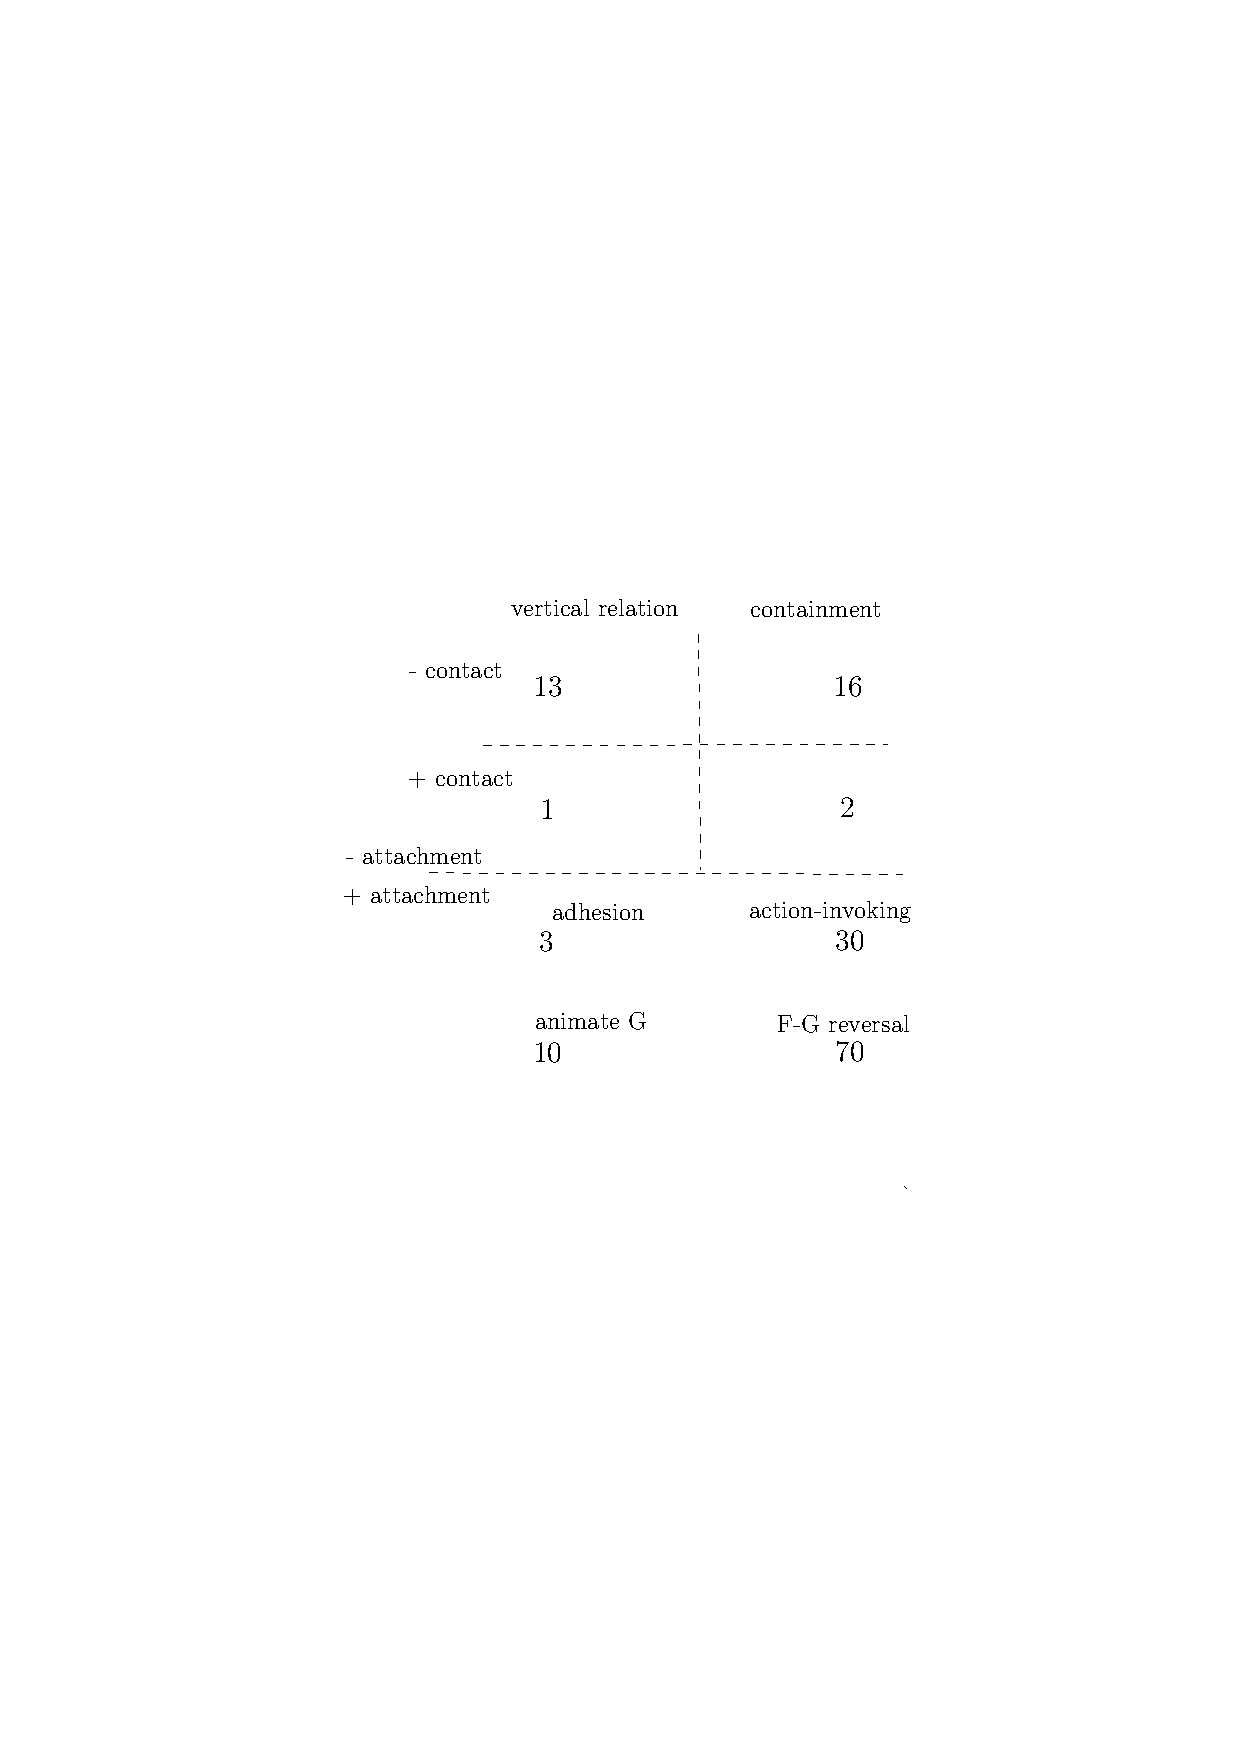
\includegraphics[width=2.2in,height=2.2in]{Graphic/Pictures/levi-top-map.pdf}
}
\qquad
 \subfloat[][Chakali topological map]{
 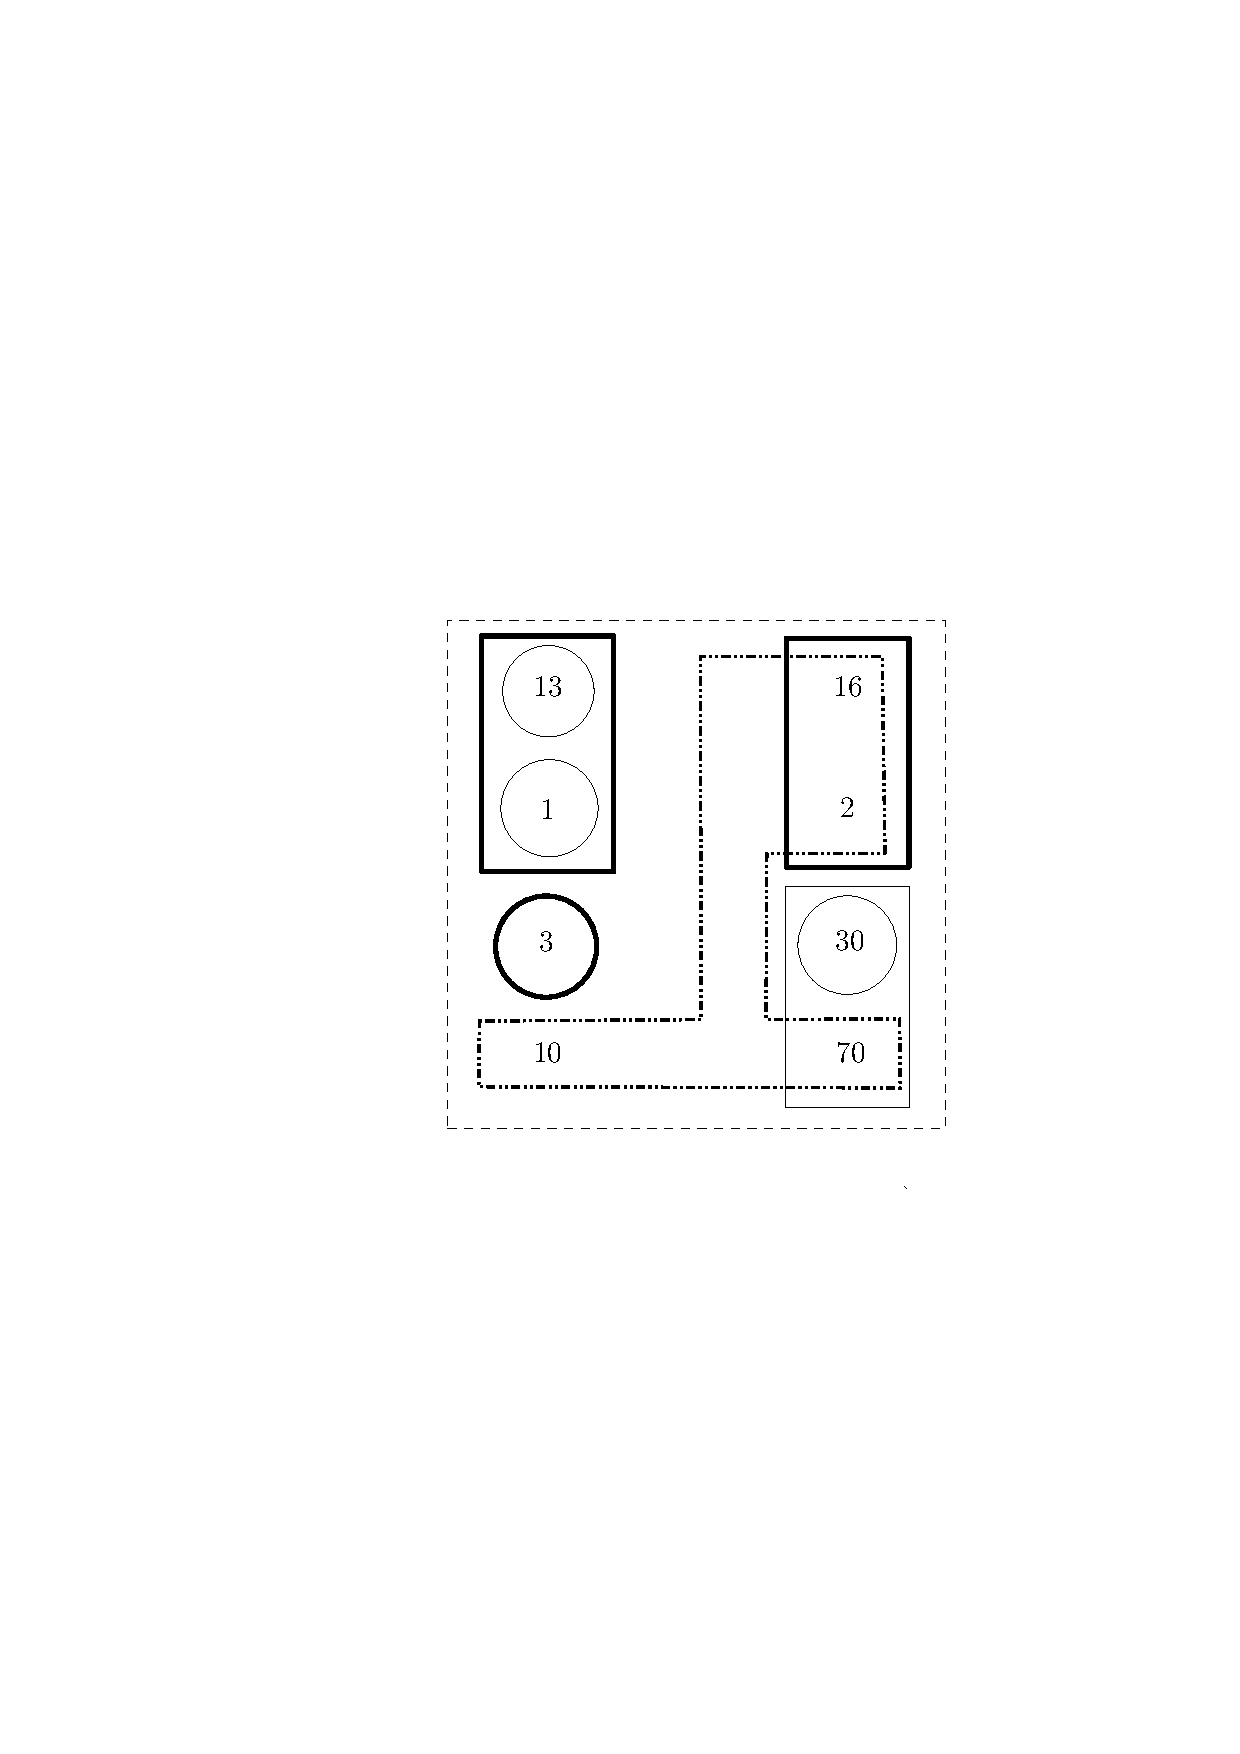
\includegraphics[width=2.2in,height=2.2in]{Graphic/Pictures/cli-top-map.pdf}
}

\caption[Stereotypical TRPS and Chakali topological map]{Stereotypical TRPS
illustrations of topological relations and Chakali topological map
\label{fig:TopoMaps}}

\end{figure}


The Chakali topological map  presented in figure \ref{fig:TopoMaps}b  encloses
the illustrations  which are described using the same linguistic expressions by
the majority of the consultants. For instance, `the fruit in the bowl' (TRPS 2)
and
`the ball under the chair' (TRPS 16) are contained in a group represented by the
expression {\S patʃɪgɪɪ}, a relational noun meaning `inside'. Both scenes
illustrate the notion of containment and non-attachment, and the reference to
such topological notions is conveyed with the relational noun {\S patʃɪgɪɪ}.
TRPS 2 and 16 are also contained in a larger group associated with the
existential verb {\S dʊa}. The nine groupings  in figure
\ref{fig:TopoMaps}
are listed in table \ref{tab:ninegroups} together with the lexical items
associated with them,  the respective part of speech
(PoS) and  English translation.  To the  nine groupings of table
\ref{tab:ninegroups}, some
observations must  be supplied to  further appreciate the type of variation
taking place. 


 \begin{table}[htb]

\caption{Groupings derived from 
 eight stereotypical TRPS illustrations
 \citep[10-11]{Levi06a}\label{tab:ninegroups}}
\centering
\begin{Itabular}{p{4cm}lll}
\Hline
Grouping &  Lexical item & PoS & English\\
\hline

1, 2, 3, 10, 13, 16, 30, 70 &  nɪ &
{\it postp} & at\\
2, 10, 16, 70  &  dʊa &\textit{v} & be
at\\
30, 70	 &   tũũ &\textit{v} & pierce\\
1, 13 	&   ɲuu &\textit{reln} & top\\
2, 16	&  patʃɪgɪɪ&\textit{reln} & inside\\
1 	& suguli &\textit{v} & be over\\
3	&   mara &\textit{v}& adhere\\
13 	&  laga &\textit{v} & hang\\
30	&   pɔ &\textit{v} & set in\\


\Hline

% <dashstyle name="dashed" value="[4] 0"/>
% <dashstyle name="dotted" value="[1 3] 0"/>
% <dashstyle name="dash dotted" value="[4 2 1 2] 0"/>
% <dashstyle name="dash dot dotted" value="[4 2 1 2 1 2] 0"/>
 
\end{Itabular} 

 \end{table} 



%and undertsand the meaning of the lexical items involved. 

% Moreover, the discussion raises a matter of doubt ion the 
% selection of the eight stereotypical illustrations.

The verb {\S suguli} in `the cup on the table' (TRPS 1) alternates with one
instance of {\S saga}. They all occur with the relational noun {\S ɲuu}. 

 \begin{exe}
 \ex\label{ex:TRPS-1}

 \gll a bonso suguli/saga a teebul ɲuu nɪ \\
{\art} cup be.over/sit  {\art} table {\reln .top} {\postp}\\
 \glt `The cup is on the table.' (TRPS 1)

 \end{exe}

According to my language consultants, all instances of {\S suguli} `be over' in
our dataset can be replaced by {\S saga} `sit', but not vice-versa. On the
whole, the verb {\S suguli} is used   to describe only the illustrations
`cup on table' (TRPS 1, also SPS 1, 2, 3, 4, 5 and 7)  and  `bottle on stone'
(PSPV 10). On the
other hand,  
the verb  {\S saga} functions as the main predicate in 47 depicted scenes.  If
the topological map intends to reflect a
stereotypical verb containing the senses  `vertical support', `with contact'
and 
`non-attachment', the evidence points at the verb {\S saga} more than at the
verb {\S
suguli}. It
seems  that {\S suguli} addresses more the ``underness'' of the ground, while 
{\S saga} concentrates on the disposition of the figure,  a default and
non-assertive disposition. One  piece of evidence
which substantiates this claim is a naming custom. The proper name {\S Suglo} is
given to a male or female newborn if he/she follows a male or female named {\S
 Ƞmaŋu}. If someone's name is {\S Suglo}, he/she is necessarily 
{\it under} a male or female sibling. In addition,  the
compound nouns {\S
viisugulii}, {\it lit.} `pot-be over', which refers 
to a  type of cooking pot which forms a stack when put together,  and {\S
dɪsugulii}, {\it lit.}  `house-be over',  which is the generic term for  
multiple floor buildings, may be used as linguistic evidence in the
identification of the meaning of   {\S suguli}. To describe many scenes,
{\S
saga}  and {\S suguli} can be used
interchangeably, and, there may possibly be conventions which restrict the use
of  {\S saga}.  Locative verbs are discussed in section
\ref{sec:SPA-post-verb}.

%in terms of rights, access to knowledge, etc.
%suguli may also code the standing of the figure?




The construction  F(igure) {\S dʊa} G(round) {\S patʃɪgɪɪ nɪ} is employed to 
express both `the
fruit in the
bowl' (TRPS 2) and `the ball under the chair'  (TRPS 16), except that in the
latter scene two consultants used the relational noun {\S muŋ} rather than  {\S
patʃɪgɪɪ}. This variation between  consultants may be due to the vagueness of
the area to identify (i.e. under the seat of chair or the volume contained
within
the four legs), in conjunction with the absence of four-legged chairs at their
respective villages.


 \begin{exe}
 \ex\label{ex:TRPS-2-16}

 \begin{xlist}
 \ex\label{ex:TRPS-2}
 \gll a daanɔ̃ŋ dʊa fala  patʃɪgɪɪ nɪ   \\
{\art} fruit be.at  calabash {\reln .inside} {\postp} \\
 \glt `The fruit is in the bowl.' (TRPS 2)

 \ex\label{ex:TRPS-16}
 \gll bɔl dʊa kor muŋ/patʃɪgɪɪ nɪ\\
ball  be.at  chair {\reln .under/inside} {\postp}  \\
 \glt `The ball is under the chair.' (TRPS 16)

 \end{xlist}
 \end{exe}

 

 The scene `the stamp on the letter'  (TRPS  3) was described with {\S mara}
by two consultants, as shown in (\ref{ex:TRPS-3}). One consultant used {\S saga}
and
the other consultant used
a non-BLC impersonal construction (see section \ref{sec:nonBLC}) with {\S
stampa} ($<$ Eng. `stamp')  acting as main predicate (i.e. {\S ba stampa a lɛta
ra} `they stamp the letter').  The verb {\S mara} is
without a doubt the predicate associated with the concept of adhesion. It is
used by all or the majority of the consultants for the scenes depicted in
`insect on ceiling' (TRPS 7),  `telephone on wall'  (TRPS 25),  `face on stamp'
 (TRPS 28) and  `insects on wall' (TRPS 52), and by two consultants for 
`stamp on envelope' (TRPS 3), `fruit on branch' (TRPS 27), `leaves on
branch' (TRPS 41), `rain on window' (TRPS 48) and `handle on door' (TRPS 61).



 \begin{exe}
 \ex\label{ex:TRPS-3}

 \gll  a stampɪ mara a tɔn nɪ\\
{\art} stamp adhere  {\art} paper {\postp} \\
 \glt `The stamp is on the letter.' (TRPS 3)

 \end{exe}


Everyone describes  the  `the ring on
the finger' (TRPS 10) with the existential predicate  {\S dʊa}. Scenes
involving animate ground are generally described by all consultants with {\S
dʊa}
(i.e. `shoe on foot' (TRPS 21), `plaster on leg' (TRPS 35),  `bandage on leg'
(TRPS 39),  `necklace around neck' (TRPS 51) and  `earring on ear' (TRPS
69)).\footnote{However, this is apart from the
verbs {\F
tʃige} `cover face down', which is used to describe the illustration where
a hat is on the head of a person (TRPS 5), and {\F vɔwa} `tie', which is used
to describe the illustration where a piece of cloth is around the waist of a
woman (TRPS 42)  and where a hair band is around the head of a person  (TRPS
46).}


 \begin{exe}
 \ex\label{ex:TRPS-10}
 \gll neŋgbiŋ dʊa nebii nɪ \\
ring be.at finger {\postp} \\
 \glt `The ring is  on the finger.' (TRPS 10)
 \end{exe}




The scene `the lamp over the table'  (TRPS  13)  illustrates a case where a
disagreement among consultants is  caused by the selection of different ground
objects. In this case, there is a division
between the consultants  who describe the scene with the verb
 {\S laga} `hang' with the ground object {\S dɪa} `house' or {\S dɪa ɲuu}
`ceiling', and those who make use of the verb {\S gaalɪ} `be over'  or {\S
 dʊgʊlɪ} `be
near' with the ground object {\S tebul} `table'. The verb {\S gaalɪ} `be
over' differs from {\S suguli} `be over' by the way they encode the notion of
`contact': with {\S gaalɪ},  the figure cannot be in contact with the ground,
 but with   {\S suguli} it must. 



 \begin{exe}
 \ex\label{ex:TRPS-13ab}
 \begin{xlist}

 \ex\label{ex:TRPS-13a}
 \gll  diŋtʃaŋ laga a dɪa (ɲuu) nɪ\\
lamp hang {\art} house {(\reln .top)} {\postp}  \\
 \glt `The lamp hangs from the house.' (TRPS 13)

 \ex\label{ex:TRPS-13b}
 \gll a diŋ dʊgʊlɪ/gaalɪ a teebul nɪ   \\
{\art} fire be.near/be.over  {\art} table  {\postp} \\
 \glt `The lamp is over the table.' (TRPS 13)
 \end{xlist}

 \end{exe}

The verb {\S  tʊ̃ʊ̃} encodes the information of  the action-evoking scene `the
arrow through the fruit' (TRPS 30) and the figure-ground reversal scene  `the
fruit pierced by the needle'  (TRPS 70), though the verb {\S pɔ} `insert' or
`set in' was used by two consultants to describe TRPS 30. Examples 
(\ref{ex:TRPS-70f-g}) and  (\ref{ex:TRPS-70g-f}) shows that the verb  {\S 
tʊ̃ʊ̃} may take either {\S daanɔ̃ŋ}  `fruit' or  {\S hembii} `nail' as
grammatical subject.


 \begin{exe}
 \ex\label{ex:TRPS-30-70}
 \begin{xlist}

 \ex\label{ex:TRPS-30}
 \gll  tobii   tʊ̃ʊ̃/pɔ a daanɔ̃ŋ  nɪ\\
 arrow pierce/plant {\sc art}   fruit {\sc postp}  \\
 \glt `The arrow is planted in the fruit.' (TRPS 30)
%fix
 \ex\label{ex:TRPS-70f-g}
 \gll  a hembii   tʊ̃ʊ̃ a daanɔ̃ŋ  nɪ \\
{\sc art} nail pierce {\sc art} fruit {\sc postp}\\
 \glt `The nail pierces the fruit.' (TRPS 70)


 \ex\label{ex:TRPS-70g-f}
 \gll a daanɔ̃ŋ   tʊ̃ʊ̃ a hembii nɪ\\
 {\sc art} fruit pierce   {\sc art} nail {\sc postp} \\
 \glt `The fruit pierces the nail.' (TRPS 70)

 \end{xlist}
 \end{exe}


To summarize, the Chakali topological map with its eight stereotypical TPRS
illustrations reveals important generalizations about the grammatical encoding
of static configurations. Still, it is an oversimplified conception. In the next
section I discuss in detail  the main components of the BLC in Chakali, that
is,  the topological relation markers.



\subsection{Topological relation markers}
\label{sec:SPA-trm}

Spatial meanings  are carried by topological relation markers (TRM), which are
``various form classes involved in encoding topological  relations''
\citep[486]{Levi03b}. In the previous sections, we saw that  topological
concepts are wholly expressed by means of  three classes of
expression:  a postposition, a series of relational nouns and a series of
locative verbs. Each of these is discussed below.



\subsubsection{The postposition {\I nɪ}}
\label{sec:SPA-postp}

%put terrill Lavulekele suffix n
Cross-linguistically,  Chakali  {\S
nɪ} shares strong similiarities with the preposition  {\S lə} 
in Sɛkpɛlé
\citep[1071]{Amek07c},
the morpheme {\S ni} in Swahili \citep{Knap67}, the particle {\S di} in
Indonesian \citep[112-114]{MacD76}, the particle  {\S gi} in Chamorro
\citep[116-119]{Topp73}, among others. 


What they have in common is that all  signal only that the
constituent in which they appear is locative. In `case' languages, a particular
case may have a similar function (e.g. locative case {\S -n} in Basque
\citep[2]{Ibar10}). Generic locative adpositions are often analyzed as the
source
of the emergence of locative case. For instance, in Lavukaleve (an isolated
member of the Solomon Islands) it may be argued that the   locative case {\S -n}
 is historically
derived from the postposition {\S na} `in' \citep[see][161]{Terr03}.\footnote{In
 searching the literature  for general locative markers across
languages of the world, it is striking that many of them contained  nasal
features. Is this an example of phonosemanticism or a simple coincidence?} For
the
most part, the postposition {\S nɪ} is found  throughout   the dataset.  In
fact, in the majority of the 900 or so utterances,  the locative
particle {\S nɪ} is present irrespective of the
locative verb involved or whether or not a relational noun occurs. Only a  few
exceptions can be found,   and they are
systematically accounted for by two factors: (i) some verbs  do not co-occur
with
the locative particle {\S nɪ}, e.g. {\S tɔ} `cover', {\S kpaga} `have' and {\S
su} `fill',  and (ii) some situations are described using an intransitive
clause, e.g.   {\S a bonso tʃiegiu}   `the cup is broken' (TRPS 26).   The
 occurrence of {\S nɪ}  resembles the role of  `be' in English, since it is
also
found in the majority of sentences describing the situations illustrated in the
stimuli. However, unlike English `be', the postposition  {\S nɪ} can neither be
replaced by another adposition nor be left unpronounced (i.e. `the cup is on the
table'  $>$   `the cup sits/stands on the table', `the cup is on the table'  $>$
 `I see the cup on the table',  `It is on the table' $>$  `On the table!').
\citet[370]{Amek06} present the Ewe verb {\S le}, glossed  `be at',  which is
used in the majority of the sentences denoting the situations of the TRPS.   The
translation of  Ewe {\S le} to Chakali would then be equivalent to {\S dʊa ...
nɪ}.\footnote{The Ewe verb {\F le} may also function as predicator of qualities
\citep[373]{Amek06}. In Chakali,  it was shown  in sections
\ref{sec:GRM-ident-cl} and \ref{sec:classifier} that   {\F
jaa} predicates over qualities,  not  {\F dʊa}.}



In Chakali the postposition {\S nɪ} identifies an oblique object phrase, and
 conveys that the oblique object phrase contains the ground object. The
complement precedes the  postposition. The examples  displayed in 
({\ref{ex:postp-corres}}) show that the complement of  {\S nɪ} is a noun phrase
(for RelP, see section \ref{sec:SPA-relnoun}). Since there are no prepositions
in the language, the abbreviation PP in ({\ref{ex:postp-corres}}) unambiguously
stands for Postposition Phrase.

\begin{exe}
\ex\label{ex:postp-corres}
 {[[[a dɪa]}_{NP} {ɲuu]}_{RelP} {nɪ]}_{PP}  `on the roof of the house' \\
{[[a dɪa]}_{NP} {nɪ]}_{PP}  `in/at the house' \\
 {[[baŋ]}_{NP} {nɪ]}_{PP}  `here'\\
{[[de]}_{NP} {nɪ]}_{PP}  `there'\\
{[[ʊ]}_{NP} {nɪ]}_{PP}  `at/on/in him/her/it'\\
\end{exe}

Nevertheless, the postposition does not inform the hearer on any of the
elementary topological spatial notions; none of the concepts of proximity,
contiguity or containment are encoded in  the postposition {\S nɪ}. It never
 selects particular figure-ground configurations but must be present for all of
them. 

Besides the description of static configurations, the postposition {\S nɪ}  is
used frequently in adverbial/connective expressions: {\S a bɔnɪɛ̃ nɪ} `maybe,
perhaps', {\S a ɲuu nɪ} `therefore', {\S buŋbuŋ nɪ} `at first', etc. These
adverbial/connective expressions do not have a purely locative function, but are
rather used as clause modifiers,  or to introduce logical conclusion. These
expressions are
at the edge of the category adverb, leaning towards those expressions treated as
connectives (see sections   \ref{GRM-clause-subord} and
\ref{sec:GRM-adjuncts}). 


% \footnote{The \cite{Jack83}' 
% notions can be taken to be either primitive, so that we have conceptual
% primes like IN, ON, UNDER Jackendoff 1983),} 


%compare Kwa and Gur
%body parts and relational nouns (see Brown)

 


\subsubsection{Relational Nouns}
\label{sec:SPA-relnoun}

%                                               Some relational nouns are de-
% rived from body parts, e.g., ..., but not all, e.g.,
% -baamban??

Many  languages present formal identity between body parts terms and expressions
used to designate elements of space. The widely accepted view is that
diachronically  spatial relational nouns (sometimes called spatial nominals
\citep[895]{Hell07} or adpositions \citep[137]{Hein97}) are ``the result of
functional split'' and that ``they are derived from nouns denoting body parts or
locative concepts through syntactic reanalysis'' \citep[256]{Hein84}. In Ewe
(Kwa) for instance, it is claimed that  the prepositions have evolved from verbs
and postpositions from nouns \citep[367-369]{Amek06}. 

% 
% In the theory of grammaticalization's terms
% \citep[137]{Hein97} 
% In  \cite{Amek06}
% it is claimed that i
% 
% What we call a relational noun has received several other labels in the
% literature; spatial nominal \citep[895]{Hell07}, postposition
% \citep[256]{Hein84}. 


Chakali relational nouns are formally identical to body part nouns although 
not all body part nouns have a relational noun counterpart. For instance,
whereas {\S
ɲuu} can have both  a spatial meaning, i.e. `on top of X', and  a body part one,
i.e. `head',  the body part terms {\S bembii} `heart', {\S hog} `bone'  or {\S
fʊ̃ʊ̃} `lower back', among others,  cannot convey  spatial meanings. Table
\ref{tab:relvsbody} displays the body parts found in the data which
convey spatial meaning.\footnote{The body part term {\F gantal}
`back' is from
the Ducie lect and corresponds to {\F habʊa} in the Motigu, Gurumbele,
Katua, Tiisa and Tuosa lects.}



\begin{table}[h!]
\caption[Spatial nominal relations and body part nouns]{Spatial nominal
relations and body part nouns: similar forms and different, but related,
meanings\label{tab:relvsbody}}
\centering
\begin{small}
 \begin{Itabular}{l|ll|ll}
\Hline
Projection& Spatial relation & PoS: {\it reln}  & Body parts &
 PoS: {\it n}\\   \hline
Intrinsic & &&&\\

& \textsc{top}  & {  ɲuu(x,y)} & head & {  ɲuu(x)}\\
&\textsc{containment} &  { patʃɪgɪɪ(x,y)}  & stomach & {
patʃɪgɪɪ(x)}\\

& \textsc{side} &  { logun(x,y)}& rib & { logun(x)}\\
& \textsc{mouth} &  { nʊã(x,y)}& mouth & { nʊã(x)}\\
& \textsc{base/under} &  { muŋ(x,y)}& arse & { muŋ(x)}\\
& \textsc{middle} &  { bambaaŋ(x,y)}& chest box & { bambaaŋ(x)}\\
\cline{1-3}

Relative  & &&&\\
& \textsc{left} &  {neŋgal(x,y)}& left hand &  {neŋgal(x)}\\
& \textsc{right}  & {nendul(x,y)}  & right hand &{nendul(x)} \\
& \textsc{back} &  {gantal(x,y)}  & dorsum & {gantal(x)}\\
&    \textsc{front} & {sʊʊ(x,y)}  & front  & {sʊʊ(x)}\\
\Hline

 \end{Itabular}
\end{small}

\end{table} 







The contrast between an intrinsic and a relative frame of reference was brought
up in section \ref{sec:SPA-exper1-sum} where we confirmed that both  an 
intrinsic and a relative exocentric and egocentric  frames of reference were
being used. An intrinsic frame of reference is  invariant no matter how the
spatial relation is viewed by the speaker or the addressee, whereas a
relative
frame of reference depends on
how a spatial relation is  viewed. 


% Sure that is right. Also suppose that you put the cutlass you used to cut the
% head on the head. Now you can say, 'a karintie saga a nyuu nyu ni'. In your
% given example, the kpulikpuli is on the head. Let's change it and say the
% kpulikpuli is under the head. Then we would have, 'a kpulikpuli dua a nyu mun
% ni'. I'm not sure how these will allow, could you give examples? gantal gantal
% 'behind the back'
% nua nua  'at the entrance of the
% mouth' pachigi pachigi 'inside the stomach' (Kasim)

How can we distinguish a relational
noun from a noun?  Above all,  the differentiation between relational
nouns and body part nouns cannot rely solely on surface syntax criteria,
precisely
because the configuration of a possessive noun phrase and a
relational noun phrase are identical. This is shown in
 (\ref{ex:SPA-reln-vs-bpn}). 

\begin{exe}
\ex\label{ex:SPA-reln-vs-bpn}
\begin{xlist}
 
\ex\label{ex:SPA-bpn}{\it Possessive attributive phrase}\\
 {[{\sc n}_{1}-{\sc n}_{2}]}_{NP} where {\sc
n}_{2}=body part,   e.g. {\S baal  ɲuu} ``a man's head''
\ex\label{ex:SPA-reln}{\it Spatial nominal  phrase}\\
 {[{\sc n}_{1}-{\sc n}_{2}]}_{NP} where {\sc
n}_{2}=spatial relation,   e.g. {\S tebul  ɲuu} ``top of the table''
\end{xlist}
\end{exe}

Even though the two corresponding nominal structures may cause ambiguities,
the
interpretation is generally disclosed by the meaning of the nominal preceding
the {\sc n}_{2} in  (\ref{ex:SPA-reln-vs-bpn}). The term  {\S  ɲuu}, for
instance, can only mean `top of' in a 
phrase in which it follows another nominal and refers to a projected
location of {\sc n}_{1}'s referent. In (\ref{ex:SPA-bpn}), even
though {\S ɲuu}
 immediately follows a nominal,  it would not normally refer to the projected
location `on the top' but only to the man's head. Nevertheless, despite any
attempts to identify  structural characteristics which may contribute to the
disambiguation of a phrase involving a body part term,  
ambiguities may still arise.


%a kpulikpuli dua a statue nyuu nyuu ni






Another aspect of body part terms is their different function in  morphological
and syntactic structure. While a relational noun is a syntactic word,  body
part terms may also function as morphemes in compound nouns to express a
specific
part-whole relationship or a conventionalized metaphor \citep[141]{Hein97}. 
Whereas the distinction may be formally and semantically hard to distinguish,
the number of body
part terms which can be the stem in a compound noun is larger than those
functioning as relational nouns. Some examples are shown in table
\ref{tab:SPA-bpt-compound}.

%fix the etymology

\begin{table}[h!]
\caption{Body part terms in compound nouns\label{tab:SPA-bpt-compound}}
\centering
%\begin{small}
 \begin{Itabular}{lllp{1.6in}}
\Hline
Body part term & Compound noun  & Morph. gloss & Gloss \\ \hline


eye &    tɔ́ʊ́|sìì  & village-eye & village's center\\
 & kpã̀ã̀n|síí & yam-eye & yam stem\\
& nɪ̀ɪ̀|síí & water-eye & deepest area of a  river\\
 &  nã̀ã̀|síí & leg-eye & ankle bump\\

 mouth 	&   gɔ́ŋə|nʊ̀ã́ & river-mouth & river bank \\
		&   ʔɪ̀l|nʊ̀ã́  & breast-mouth& nipple \\
                &   dɪ́à|nʊ́ã̀& house-mouth& door \\

leg &   gɔ́n|nã́ã́   & river-leg & split of a river  \\ 

&   dáá|nã̀ã̀  & tree-leg & branch\\




 head &   kùósò|ɲúù  & god-head & sky\\
             &   tìì|ɲúù  &land-head  ({\G etym})& west\\
%stomach&   \S tɔ̀ʊ́pàtʃɪ́gɪ́ɪ́  & village-stomach & inside the village\\

 arse &  tìì|múŋ &land-arse  ({\G etym}) & east \\

neck &  vìì|báɣəná & pot-neck & neck of a container\\

testicle &   mááfà|lúrò  &  gun-testicle &  gun powder container\\

penis &  mááfà|péŋ  & gun-penis &gun trigger\\

ear &   mááfà|dɪ́gɪ́ná   & gun-ear & flintlock frizzen \\

arm &  fálánèŋ & calabash-arm & calabash stem\\
 
navel & fálá|ʔúl & calabash-navel & calabash node\\

nose & píí|mɪ́ɪ́sà & yam mound-nose &  part of a yam mound\\
liver & tɔ́ʊ́|pʊ̀ɔ̀l & village-liver &  important community member\\
\Hline
 \end{Itabular}
%\end{small}

\end{table} 

Ignoring for the moment the structure in which they are involved, there seem to
be two types
of spatial interpretation accessible with body part terms. And there also seems
to be a gray zone between the two.\footnote{This gray zone may receive a
diachronic interpretation.  In
\citet[1072]{Amek07c},  the postpositions in Sɛkpɛlé are seen as evolving
``from body part and environment terms''  and have a similar, but not
identical, 
function as those of Chakali relational nouns. For instance, Sɛkpɛlé's  
postpositions ``cannot be modified'' nor can they vary ``with respect to number
 marking''.  As we shall see below, the latter property is not applicable to
Chakali relational nouns. The former is undetermined as I do not know what
counts as a `modified postposition'.} The first interpretation is the literal
attribution of human
characteristics (i.e. anthropomorphic) in  reference to parts of object. In a
such a
case, a body part term refers to a part of an object in analogy to an animate
entity. For instance, a trigger of a gun (i.e. the lever that activates the
firing
mechanism) is  attributed to the penis to characterize its physical appearance.
The
second interpretation does not designate a fixed part of an object
but a location projected from a part of an object.  In such a case it designates
a spatial environment in contact with or detached from an object
\citep[44]{Hein97}. To make the
distinction clear,  in the sentence `a label is glued on the neck of the bottle'
the body part term {\it neck} designates a breakable part of the bottle, whereas
in the sentence `John is standing at the back of the car' the body part term
{\it back} does not designate any part of the car but a relative spatial
location, the area behind the car. 


 In \citet[44]{Hein97}, the variety of denotations of body part terms is
accounted for in a diachronic perspective. The  claim is sketched in
(\ref{ex:Heine-stage}).


\begin{exe}
\ex\label{ex:Heine-stage}{\it From body part to spatial concept: A four-stage
scenario \citep[44]{Hein97}}\\
Stage 1: a region of the human body\\
Stage 2: a region of an (inanimate) object\\
Stage 3: a region in contact with the object\\ 
Stage 4:  a region detached from the object\\
\end{exe}


However, synchronically each of these stages is observable: A  Chakali 
relational noun is more easily interpreted as  a region in contact with or
detached from an object, a body part term in a compound
noun designates
a part of an object, and a body part term used as
a full-fledged noun is associated with a part of the human body. 
Nevertheless, the examples provided in table \ref{tab:SPA-bpt-compound} show
that the distinction is not a clear-cut one: Does the expression {\S tebul ɲuu}
designate a spatial environment  in contact with or detached from a table or  a
part of table? Both interpretations seem acceptable.

% For instance, {\S dáámúŋ}, literally `tree under', can  mean either a
% resting area or a location for the initiation rite (neither being obligatorily
% under a tree), and the sentence {\S ʊ dʊa daa muŋ nɪ} can only be interpreted
%as
% `it is under the tree', but never as `it is at the resting area' nor as  `it
%is
% at the location for the initiation rite'.
Relational nouns
are rarely found in their plural form: but on grammatical grounds, nothing
prevents them from being expressed in the plural. 
To describe a situation where  for every bench there is a calabash sitting on
it, 
the sentence in (\ref{ex:reln-plu-head}) is appropirate.


\begin{exe}
\ex\label{ex:reln-plu-head}
\gll falasa saga a koro ɲuuno nɪ \\
calabash.{\pl}  sit {\art} bench.{\pl}  {\reln .\pl} {\postp}\\
\glt `The calabashes sit on top of the benches.' 
\end{exe} 

One may argue that the `top of a bench' is a spatial environment  in contact
with the bench, even a physical part of the bench, so pluralization may simply
suggest that the   `top of a bench' is a word refering to an entity,  and not a
locative phrase. Two pieces of evidence go against this view: first,  notice
that {\S koro} `bench'  in {\S koro ɲuuno} is plural.  Recall section
\ref{sec:GRM-com-stem-noun} in which a noun class ({\it sg./pl.} marking) was
argued to  appear only at the end of a word. If  `top of a bench' was a word and
not a phrase, we would expect its plural form to be  *{\S korɲuuno}. Secondly, 
deciding whether or not the `top of' is indeed in contact with or detached from
the bench is not conclusive. To describe a situation where several balls are
under several tables, one may use the sentence in (\ref{ex:reln-plu-stomach}), 
in which case it cannot be argued that  under of the table is a physical part of
the table.\footnote{One may argue that it is indeed a part of the table,
identical to the interior space of a container.}

\begin{exe}
\ex\label{ex:reln-plu-stomach}
\gll a bɔlsa dʊa tebulso patʃɪgɪɛ nɪ  \\
{\art} ball.{\pl}  be.at  table.{\pl}  {\reln .\pl} {\postp}\\
\glt `The balls are under the tables.'
\end{exe} 



% kopu suguli a tebul nyu- logun ni
% a haan dua u gantal ni 'the woman is at his back'
% The above sentences are right. But in the case of "a haana dua ba gantala ni"
%we  only pularise the subject (haana) but keep the location (gantal) singular
% because 'ba' has already indicated that they are many. So we have 'a haana dua
% ba gantal ni' NOT 'a haana dua ba gantala ni'. However, a balsa dua tebulSO
% pachigiE ni is right. Why because, we are referring to objects and not humans
%in  which case we cannot use 'ba' indicate it's a single object or many. For
% instance, we can have " a fota saga dasa nyuuni ni" (the baboons are on the
% trees) 'a zinni laga da nyu ni' (the bats are hanging on a tree).

Another aspect of relational nouns and oblique phrases in general is that
they are structurally very rigid, that is, one does not usually extract from
them nor does
one preposes the oblique object phrase or elements from the phrase. Although
rarely
topicalized, the
sentences in  (\ref{ex:reln-extract-in-1})  is acceptable. 

%other charac: conjunction

\begin{exe}
\ex\label{ex:reln-extract}
\begin{xlist}
 \ex\label{ex:reln-extract-in-1}

\gll  a tebul  ɲuu nɪ, a fala saga  \\
 {\art } table {\reln} {\postp}  {\art } calabash sit\\
\glt `On top of the table, the calabash sits.'

 \ex\label{ex:reln-extract-in-2}
\gll  tebul lo, a fala saga ʊ   ɲuu nɪ  \\
 table {\foc} {\art} calabash sit {3.\sg.\poss} {\reln. top} {\postp}   \\
\glt `Table, the calabash sits on top of it.' ({\it lit.} `sits on its head')
 \ex\label{ex:reln-extract-out-3}
* tebul lo, a fala saga  ɲuu nɪ
 \ex\label{ex:reln-extract-out-1}
 * ʊ   ɲuu nɪ, a fala saga tebul
 \ex\label{ex:reln-extract-out-2}
 *   ɲuu nɪ, a fala saga tebul

\end{xlist}
\end{exe} 


The sentence in  (\ref{ex:reln-extract-in-2}) is acceptable but odd. It shows
that the nominal complement of the relational noun
{\S ɲuu} can be uttered at the beginning of the sentence while the possessive
pronoun {\S ʊ}  is located  in the complement slot of   the relational noun, 
functioning as anaphora. The sentence is ungrammatical if the
pronoun is absent {\it in situ} (\ref{ex:reln-extract-out-3}),  or if the
oblique object phrase is preposed but the nominal {\S tebul} stranded, whether
an anaphora referring to {\S
tebul} is present  (\ref{ex:reln-extract-out-1}) or absent
(\ref{ex:reln-extract-out-2}). 



We now have  evidence for treating the relational nouns as
members of a closed class of lexical items whose function is to localize the
figure to a
search domain.  It is not only that body part terms acquire spatial meaning
following a noun referring to inanimate entities, but that, in diachrony, 
only a limited set of body part
terms has acquired that spatial meaning,  and, in synchrony, 
they form a subtype of nominal identified as relational noun. They are 
nouns since they can pluralize, but they acquire the status of functional words
since they constitute a formal class with limited membership where each of
the members expresses spatial meaning and requires a nominal complement.

\begin{exe}
\ex\label{ex:postp-struct}
 [[[a dɪa]_{NP} ɲuu]_{RelP} nɪ]_{PP}  `on the roof of the house' 
\end{exe}

In the structure  of the BLC oblique  phrase  in
(\ref{ex:postp-struct}), the relational noun {\S ɲuu}
is within the complement phrase of the postposition {\S nɪ}.  A relational noun
phrase (RelP)
 consists of a head  and noun phrase
complement.\footnote{Following recent
work in theoretical syntax in the minimalism
framework,
relational nouns fit well into what \cite{Sven08a, Sven08} calls AxPart. The
structure in (\ref{ex:postp-struct}) would then receive the graph
representation \begin{center}
{\F
  \Tree{  &&\Kq{ Place}\Bq{dl}\Bq{dr} &\\
& \Kq{ AxPart}\Bq{dl}\Bq{dr} && \Kq{\F nɪ}\\
 \Kq{ D}&  &\Kq{\it reln} &} \\
}\end{center} in which  D would be the projection of a nominal expression
denoting the
ground
element, the relational noun would take the Axpart position, a position
occupied by a linguistic item whose meaning points at a subregion of the
ground element by narrowing down the search
domain. The Place node  would always be associated with the postposition {\F
nɪ}.}  We are now in a  better position to state that the complement phrase of
the postposition is a (nominal) phrase which corresponds to the
conceptual ground. 


To summarize, on a diachronical basis, it is believed that the function of 
relational nouns  as locative adpositions originates from their purely `entity'
meaning
through grammaticalization \cite[44, 83]{Hein84}. The form of Chakali body part
terms supports the claim.   On a synchronical basis, only  {\S patʃɪgɪɪ}
`stomach',  {\S logun } `rib',  {\S gantal} `dorso', {\S muŋ}   `arse', {\S
nʊã} `mouth',  {\S sʊʊ} `front', {\S bambaaŋ} `chest box'  and {\S ɲuu} `head'
are relational nouns. Relational nouns are  nouns which lack the 
referential power of the default interpretation of  body part term  (i.e.
interpreted in  isolation), and which take a
complement which must obligatorily be filled by an entity capable of projecting
a spatial environment.

%\cite[137]{Hein97}
%inherent vs. relative spatial terms
%check with Linguistic Semantic book, examples...

\subsubsection{Locative verbs}
\label{sec:SPA-post-verb}

%               These have ratherdifferent semantic properties, so that, for
% example, the small sets have
% classifying or presuppositionaluses (the figure need not be in the canonical
% posture), while the large sets
% have primarilyassertionaluses.


Table \ref{tab:Amek-typology-loc-verb} displays the  typological
classification of locative predication  proposed by \cite{Amek07b},  a typology
which classifies languages according to their verbal component in BLC. 


\begin{table}[h]
\caption[Types of locative predication]{Types of locative
predication (verbal
component) in basic locative construction (BLC).  Reproduction and adaptation
of \citet[863-864]{Amek07b}  \label{tab:Amek-typology-loc-verb}}

 \centering
\begin{Itabular}{llp{7cm}}
\Hline
Type 0 &  & No verb in BLC ({\it Saliba})\\
\hline
Type I &  & Single locative verb (or suppletion under grammatical
conditioning)\\
 & Ia &  Copula ({\it English, Tamil, Chukchi, Tiriyó})\\
 & Ib & Locative (+Existential) verb ({\it Japanese, Ewe, Yukatek,
Lavukaleve})\\
\hline
Type II &  & A small contrastive set of locative verbs (3-7 verbs) \\
 & IIa & Postural verbs ({\it Arrernte, Dutch, Goemai})\\
 & IIb & Ground space indicating verbs ({\it Tidore}) \\
\hline
Type III &  & Multiverb Positional verbs (a large set of dispositional verbs,
9-100) ({\it Tzeltal, Zapotec, German, Laz, Sɛkpɛlé})\\
\Hline
\end{Itabular}
\end{table}

Even though \citeauthor{Amek07b}  provide language-tokens  for each type, they
write that languages may show  important variations and subtleties. For
instance, a speaker may use two different strategies and  these strategies may
be  of different type in the classification. They write that ``Tidore  ...
provides evidence for a distinction between a small-set type and a multiverb
type as it has in addition to the seven Ground space indicating locational
verbs, twenty or so dispositional and configurational verbs''
(\citet[863]{Amek07b}, based on \cite{vanS07}).  Goemai also presents
``language-internal evidence for the existence of two different types of
locative verbs''  \citep[893]{Hell07}.  However, \citeauthor{Amek07b}  claim
that, overall, languages tend to follow their typology \citep[867]{Amek07b}.  In
the  sections to come, I  show that the characteristics of the verbal component
in the BLC  point to the classification of Chakali into Type III. 




\begin{figure}[h]
\centering

 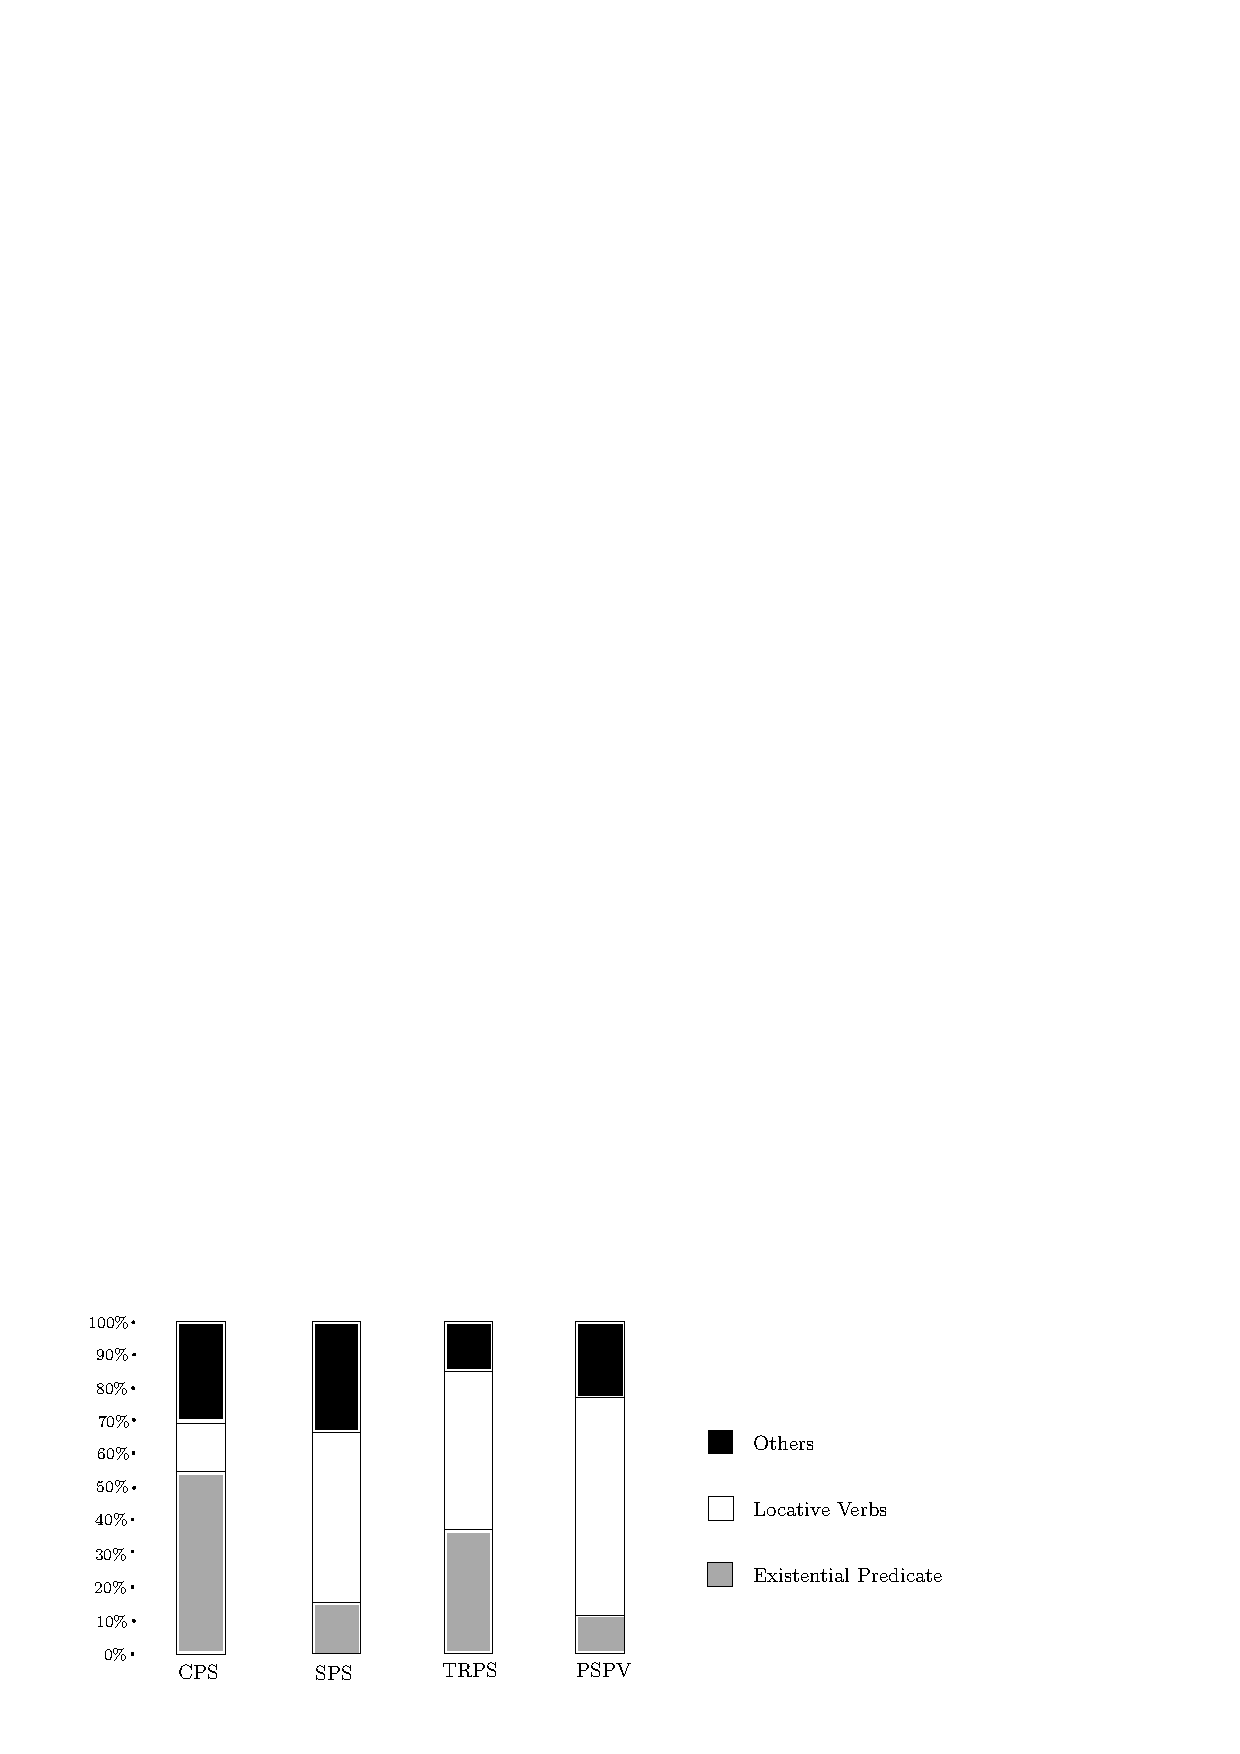
\includegraphics[width=10cm]{Graphic/Pictures/figure-verb-space.pdf}

\caption[Percentage of response types for the  four stimuli CPS, SPS, TRPS and
PSPV]{Percentage of response types for the  four stimuli CPS, SPS, TRPS and
PSPV. Existential predicate = gray bar, Locative verbs = white bar, Others =
black bar [N=CPS 164, SPS 188, TRPS 284, PSPV 272]\label{fig:exist-loc-other}}
\end{figure} 

Figure \ref{fig:exist-loc-other} acts as a  synopsis for  the elaboration in 
subsequent sections. It  displays the percentage of response types
in three groups for the four stimuli:  responses containing the existential
predicate {\S dʊa} are represented in gray, responses containing a locative
verb
 are in white and others in black.  It shows that
the  frequency of the  existential  predicate  is higher for the CPS stimulus
(55\%) than the  TRPS stimulus (34\%).  Only 15\% and 11\% of the responses in
the
SPS and PSPV respectively contained
existential predicate {\S dʊa}. Locative verbs were used in 70\% of the
responses in the PSPV stimulus, followed by  56\%, 50\% and 14\% of the
responses for the SPS, TRPS and CPS respectively. Responses labelled `Others'
are defined as follow: The original data was normalized  in order to promote the
degree  of consensus among participants. This was done by associating each
illustration with a verb or verbs which showed at least 50\% consensus. As a
result,   the illustration `food in plate' (CPS 25) is associated with {\S
saga}
and {\S dʊa} since  two consultants uttered the former and the two others the
latter,  and the illustration `worm in fruit' (CPS 31) is associated only with
{\S dʊa} since  all four consultants used this verb. As a result, the
normalization procedure can treat a response
containing the existential predicate or a locative verb as an `Others'-response
type.   One example is
how the procedure handles the
responses to the picture `stick standing on tree stump' (PSPV 38) where three
consultants used the verb {\S pɔ} and one {\S tʃɪŋa}. In this example,  the verb
{\S
pɔ} ends up
in the locative verb-response type, while  the verb {\S tʃɪŋa} in
 `Others'-response
type.  Moreover, if four different verbs are used to describe an
illustration, they all
end up in `Others' because of the normalization procedure.   Thus,
responses labelled as `Others' may contain existential  predicates or locative
verbs. I believe that putting the priority on consensus untangles in a
significant way the original data, which is highly variable and dependent upon
several uncontrolled variables. In the following sections,  the existential
predicate {\S dʊa} or a set of  locative verbs are discussed.



\paragraph{The existential predicate {\P dʊa} `be at'}
\label{sec:SPA-Type-II}

In the typology proposed in  \cite{Amek07b},  languages of Type II and Type III
are languages with a small set of contrastive locative verbs and a large set of
dispositional verbs respectively. A characteristic both types share is the
presence of one more general verb which can be used ``if none of the more
specific positional verbs is relevant'' \citep[858]{Amek07b}. In Chakali, the
existential predicate {\S dʊa} plays exactly  this role. In table
\ref{tab:SPA-exist-pred-across} the illustrations which are described using the
verb {\S dʊa} by the majority of the consultants  are presented.

\begin{table}[htb]
\caption{Four stimuli illustrations/pictures  described with the existential
predicate {\C dʊa} by the majority of the consultants
\label{tab:SPA-exist-pred-across}}
\centering
 \begin{Itabular}{lp{7cm}}
\Hline
Stimulus & Illustrations\\ \hline
CPS & 1, 4, 7, 8, 9, 11, 12, 14, 15, 18, 20, 21, 22, 23, 24, 26, 28, 31, 34,
37, 38, 40\\   \hline
TRPS & 2, 10, 11, 14, 16, 18, 19, 21, 24, 32, 39, 51, 54, 66, 67, 68, 69\\
\hline 
SPS & 12, 13, 14, 16, 21, 22, 46   \\  \hline
PSPV &  5, 22, 53, 56, 60, 62 \\
  \Hline 
 \end{Itabular}
\end{table} 

The reason why the existential predicate {\S dʊa} is deployed more in the
stimulus targeting containment (CPS) is that the existential predicate  {\S dʊa}
together with the
relational noun {\S patʃɪgɪɪ} describe containment situations adequately. 
Other sorts of
information may be  viewed as secondary by the consultants.  
And since the notion of containment is only encoded in the
relational noun {\S patʃɪgɪɪ} and since the BLC obligatorily  requires  a
verb, the existential predicate {\S dʊa} is the candidate which applies to most
situations.

\begin{exe}
\ex\label{ex:SPA-cont-PSPV22-62}
\gll kɔlba dʊa kʊzaa patʃɪgɪɪ nɪ\\
bottle be.at basket {\reln} {\postp}\\
\glt `The bottle is in the basket.' (PSPV 22, PSPV 62)
\end{exe} 

Example (\ref{ex:SPA-cont-PSPV22-62}) shows that in fact the
containment scenes `bottle lies in basket' (PSPV 22) and `bottle stands in
basket' (PSPV 62) are both described with the BLC {\S F dʊa G patʃɪgɪɪ nɪ}, even
though {\S tʃʊa} `lie' and {\S tʃɪŋa} `stand' respectively would be more
precise. Note that the relational noun {\S patʃɪgɪɪ} is  indeed compatible with
other verbs, as (\ref{ex:SPA-cont-pos-ver})  illustrates.

\begin{exe}
\ex\label{ex:SPA-cont-pos-ver}
\begin{xlist}
\ex\label{ex:SPA-cont-pos-ver-CPS-14}
bie {\S tʃʊa} a hããŋ {\S patʃɪgɪɪ} nɪ  `A baby lies in the woman' (CPS 14)
\ex\label{ex:SPA-cont-pos-ver-CPS-15}
daanɔ̃na  {\S su} a fala {\S patʃɪgɪɪ}  `Fruits fill a bowl'  (CPS 15)
\ex\label{ex:SPA-cont-pos-ver-CPS-35}
daawie {\S tele} fala {\S patʃɪgɪɪ} nɪ   `A stick leans in a bowl' (CPS 35)
\end{xlist}
\end{exe}

Likewise,  the existential predicate {\S dʊa} is  used extensively in the TRPS.
There again,  it co-occurs with the relational nouns  {\S patʃɪgɪɪ}, {\S muŋ}
and {\S
ɲuu}, and expresses
`be in', `be under' and `be on top of' respectively,  to describe the
illustrations `fruit in bowl' (TRPS 2),  `box in bag' (TRPS 14),  `ball under
chair' (TRPS 16), `fruit in ring' (TRPS 19),  `spoon under napkin' (TRPS 24), 
`fish in bowl' (TRPS 32), `cigarette in mouth' (TRPS 39) and `rabbit in cage'
(TRPS 54). The other illustrations of
the TRPS described using the existential predicate {\S dʊa} are those depicting 
`ring on finger' (TRPS 10, {\it animate ground}), `holes in cloth' (TRPS 18,
{\it negative space}), `shoe on foot' (TRPS 21,  {\it animate ground}),
`necklace on neck' (TRPS 51, {\it animate ground}), `letters on shirt' (TRPS 68,
{\it firm attachment}) and `earing on ear' (TRPS-69,  {\it animate ground}).
Those scenes are  less  likely to be expressed with a BLC according to the BLC
hierarchy \citep[15-17, 514-519]{Levi06}.\footnote{The BLC hierarchy is the 
categorization of  fifty scenes interpreted in an implicational scale
\citep[514-519]{Levi06}. Thus situations depicting piercing (level I), firm
attachment/encirclement (level II), negative space (level III), part/whole
(level IV), clothing/adornment (level V) and movable objects (level VI) are seen
as the less likely  (i.e. level I)  to the more likely (i.e. level VI) to be
expressed with a BLC. I did not carefully study  the correctness of the BLC
hierarchy in Chakali. Still, it seems to hold   as the  illustrations depicting
level I and II (i.e. TRPS 3, 4, 15, 20, 22, 23, 28, 60) are mostly described
with either a non-BLC or with {\F dʊa}, the least specific (and more general)
verb.}


\paragraph{Locative verbs: a note on terminologies}
\label{sec:SPA-posi-post-v}


The typology proposed in  \cite{Amek07b}  makes a distinction between  {\it
locative} verbs, {\it postural} verbs and   {\it dispositional} verbs (see table
\ref{tab:Amek-typology-loc-verb}).  In this work I treat the former as a
hypernym of the other two. A postural verb can be defined as
a verb which establishes  a locative relation with a ground and  codes in one
way or another the axis of a figure with respect to a ground.   They are
designated in this way since they are often seen as form-meanings derived from
human postures \citep{Newm02}. For instance, verbs of sitting, lying and
standing are common locative verbs cross-linguistically which can apply to
other objects than human ones. Dispositional verbs receive a definition in
\citet[1107-1108]{Bohn07}. The authors make a further distinction between
dispositional,
which is intended to identify a formal class of lexical items, and disposition,
which stands as a ``cover term for putative core meaning''  (i.e.
conceptual/semantic features). In \citet[909]{Hell07}, among others, one
can
find {\it positional} verbs which ``do not necessarily establish a locative
relation with the ground, but may participate or stand alone as the main BLC
predication.'' A positional verb is said to encode an internal disposition of
the
figure, but no information on the ground, and it may be preferred to  describe
the
figure in a non-canonical way. 

Even though the distinctions are important tools
of description heuristics,   they are nevertheless unnecessary
for what I want to demonstrate at this point. This is because the focus here
coincides with that of  \citet[848]{Amek07b} who state that ``our interest is
on the
synchronic patterning of these locative verbs, and (...) the semantic contrasts
they make''.  Whether or not the result suggests a distinction within the
locative verbs, the goal is primarily to (in)validate the typology introduced
above and perhaps customize it with Chakali results. From now on, no 
distinctions are assumed, but I identify sitting, lying
and standing verbs as posture verbs (section \ref{sec:SPA-post-v}). Secondly,
given that the four stimuli focus on a variety of static
configurations, I expect  the verbal elements of the BLC to reflect the variety
of situations depicted. At the same time, a set of verbs should be clearly
distinguished, not from an a priori classification, but from a careful
 semantic clustering of the verbs elicited using the four stimuli. Let us
now
uncover the
locative verbs.



\begin{table}[htbp]
\centering
\caption{Locative verbs and associated PSPV illustrations number
 \label{tab:PSPV-most-com}}
\begin{Itabular}{lp{7cm}}
\Hline
 Verb & Postural Verbs Picture Series  \\  \hline
saga & 4, 6, 8, 14, 16, 17, 18, 19, 21, 23, 24, 32, 34, 35, 44, 46, 47, 48,
50,
54, 63, 64, 66 \\
tʃʊa & 7, 11, 39, 40, 42, 51, 52  \\
%dʊa & 5, 22, 53, 56, 60, 62   \\
tele & 1,  13, 31, 65 \\
tʃige & 12, 29, 67 \\ 
vɔwa & 15 \\
tʃɪŋa & 20 \\
tɔ & 30 \\
laga & 33\\
pɔ & 38 \\

\Hline
\end{Itabular}
\end{table}






Among the four stimuli, the PSPV stimulus was specifically designed to ``aid
researchers working
especially on languages of Type II and III identify the relevant verbs'' and
``assist [us] in getting a clearer understanding of the uses, dimensions and
prototype structure of positional or spatial configurational verbs'' 
\cite[48]{Amek99}. In table
\ref{tab:PSPV-most-com},   I present the distribution of locative  verbs in
the PSPV stimulus. The second column displays the illustrations which
were identified with the verb of the first column by at least 3 consultants.
Thus, table \ref{tab:PSPV-most-com} also accounts for how well people agree in
giving a certain expression to a stimulus, that is, only illustrations which
 elicited a common verb by the
majority are included. 



The most frequent locative verb uttered in the PSPV stimulus is {\S saga} `sit'
or `be on',  followed by {\S  tʃʊa} `lie', {\S tele} `lean',
{\S tʃige} `sit face down', {\S vɔwa} `attach', {\S tʃɪŋa} `stand', {\S tɔ}
`cover', {\S laga} `suspend' and {\S pɔ} `insert'.  However, if the results of
the four stimuli are merged, the prevailing verbs expressing  spatial
configuration amount to 12-19.  They appear in the first
column of table \ref{tab:locative-verb}, followed from left to right by
the number of illustrations described with a common verb by all consultants, by
three
consultants and two consultants respectively. 


\begin{table}[htbp]
\centering
 
\caption{Locative verbs and number of illustration 
described \label{tab:locative-verb}}

\begin{Itabular}{llll}
\Hline
Locative verbs & 4/4 & 3/4 & 2/4\\

\hline
saga&13 &14 & 6 \\
saŋa& 4&0 & 1 \\
tele& 4&2 &0 \\
mara&4& 4& 3 \\
tʃʊa&4 &4 &0 \\
pɔ & 3&2 &3 \\
vɔwa&3 &5 &0 \\
tʃige& 3& 1&0 \\
laga&3 & 2&2 \\
tʃɪŋa &2&3&2 \\
tʊ̃ʊ̃&1 &0 &6 \\
tɔ& 1&2 & 0\\
suguli&0 &3 &2 \\
go(ro)& 0&1 &1 \\
kagalɛ &0 &0 & 1\\
tʃawa &0 &0 & 0\\
gaalɪ&0 &0 & 0\\
bɛra&0 &0 & 0\\
dʊgʊlɪ&0 &0 & 0\\


\Hline
\end{Itabular}
 \end{table} 





Apart from its property of 
establishing a locative relation with a ground,  a verb is selected to appear
in table  \ref{tab:locative-verb}  based on  two criteria:  (i)  all consultants
describe at
least one static configuration with the same verb (i.e. second column of
table  \ref{tab:locative-verb}),  or (ii)  its meaning and consistency in the
dataset suggest that it must be part of the set, even if it  does
not reflect a consensus among consultants.  Accordingly,  the bottom of table
 \ref{tab:locative-verb}  shows that the verb {\S dʊgʊlɪ} `be near'  is
used to
describe no illustration by either four, three or two consultants. So why
include
it, or any other  verb displaying such a low  consensus? First,
with a meaning equivalent to English `be near', the verb
{\S dʊgʊlɪ} 
clearly establishes a locative relation with a ground: it is a locative verb
expressing a propinquity relation \cite[1086]{Amek07c}.  The verb
{\S dʊgʊlɪ} `be near' is included not on the basis of a consensus among the four
speakers, but on the basis of its meaning. 
 Secondly, the existence of  locative verbs which allow more  precise
characterization,  together with the design of the
stimuli,  may contribute to the scarcity  of {\S dʊgʊlɪ}  `be near'   in the
dataset. Consider the examples in 
(\ref{ex:be-near}), which  were uttered by two different consultants. 



\begin{exe}
\ex\label{ex:be-near}
 \begin{xlist}
  \ex\label{ex:}
\gll daanɔ̃n dʊgʊlɪ a fala nʊã nɪ\\
fruit be.near {\art} calabash {\reln}  {\postp}\\
\glt `A fruit is near the calabash.' (CPS 6)%DK
 \ex\label{ex:}
\gll taal dʊgʊlɪ a bɪɪ nɪ \\
 cloud be.near   {\art} hill  {\postp} \\
\glt `A cloud is near the hill.' (TRPS 36)%Afia
 \ex\label{ex:}
\gll vaa  dʊgʊlɪ a dɪa nɪ ra   \\
dog be.near {\art} house {\postp} {\foc}\\
\glt `A dog is near the house.' (TRPS 6)%Afia
 \end{xlist}
\end{exe}

The verb {\S dʊgʊlɪ}  `be near'  is  outranked by {\S
toguni}  `squat' for TRPS 6, but  each of the illustrations TRPS 36 and CPS 6
is  described using four different verbs. This shows that the verb {\S dʊgʊlɪ} 
`be near' is mainly reported in situations with low consensus, but  that it is
indeed
a locative verb.



Also towards the bottom of   table
 \ref{tab:locative-verb},  the verb   {\S go(ro)} is triggered by 
situations depicting an  `enclosure'-relation,
i.e. mainly `fence around house' (TRPS
15) and `rope around stump' (PSPV 36). The other verbs which never show 
unanimity and are relatively
infrequent are {\S suguli} `be on', {\S gaalɪ} `hang', {\S toguni} `squat',  {\S
guti} `coil', 
{\S  tʃara} `straddle' and  {\S tʃawa} `hold', all of  which we shall return to
below.  



\paragraph{Posture verbs}
\label{sec:SPA-post-v}


The locative verbs {\S saga} `sit',  {\S tʃʊa} `lie' and {\S tʃɪŋa} `stand'
establish a locative relation with a ground and  code  axial-information of the
figure with respect to the ground. The  verb {\S saga} `sit' takes as figure
objects with either no major axis (e.g. ball) or objects with wide base in
canonical position (e.g.  stick, folded cloth, rope, pot, cassava).  An object
functioning as figure of the verb {\S tʃʊa}  has typically long axis in
canonical horizontal position (e.g. bottle, cassava), whereas an object-figure
of the verb {\S tʃɪŋa} has long axis in canonical vertical position (e.g. 
stick,  bottle). 


These generalizations account for the scene where three bottles
are standing and four are lying on a table (PSPV 46): three consultants used {\S
kɔlbasa saga tebul ɲuu nɪ} `bottles sit on top of a table', i.e. no major axis
can be identified.  Compare this situation with PSPV 52 in which all the bottles
are lying: the majority described it with {\S a kɔlbasa tʃʊa a tebul ɲuu nɪ}.
While the default collocation of  the figure object  `bottle' and the verb is
unclear from the distribution in table  \ref{tab:post-verb}, we can hypothesize
that {\S saga} is  the default locative verb used to depict the PSPV. That is
because if   {\S tʃɪŋa} `stand' is assumed to be the default collocation verb
for `bottle', then we must accept that the majority  of the consultants
presupposed the orientation of the bottle in PSPV 37 and  assert its location
with the default verb {\S saga}. But it is preferable to assume that {\S saga}
is the default collocation verb, and that  {\S tʃɪŋa} is used by only one
consultant to assert the bottle's orientation in PSPV 37.  

While the  forms for `stand' and `lie' are identical whatever the animacy of
the object-figure, a contrast exists between animate and non-animate entities
for 
the `sit' verb.\footnote{Evidence for the animacy distinction
comes from sentences where both humans and birds co-occur with the verb {\F
saŋa}. On the other hand,  the verb {\F saga} may also be used for birds, but
never for humans. Since there are no strong figures suggesting one or the other,
it seems that animacy as a sortal characteristic is indistinct, ranging from 
+human/-human, to +animate/-animate. 

\begin{exe}
\sn[]{
\gll a zimbie saŋa/saga a daa ɲuu nɪ\\ 
 {\art} bird sit  {\art} tree {\reln} {\postp}\\
\glt `A bird sits on top of the tree.' (CPS 16)}
\end{exe} 

\begin{exe}
\sn[]{
\gll daakʊã  {saŋa/saga} daa nɪ\\ 
 {bird.(type of)}  sit  tree {\postp} \\
\glt `A parrot sits on a tree.' (SPS 26)}
\end{exe} 
}


\begin{table}[ht]
\centering
\caption[Choice of locative verbs among four consultants for the scenes
depicted
by PSPV 37, 46 and 52]{Choice of locative verbs of four
consultants for the scenes depicted
by PSPV 37, 46 and 52: figure=bottle(s) and ground=table. \label{tab:post-verb}}
\begin{Itabular}{p{5cm}|llll}
\Hline
Scene (PSPV no.) &  saga `sit' &   tʃʊa `lie' &   tʃɪŋa `stand' & suguli `be.on'
 \\
\hline
1 bottle stands on table (PSPV 37)  &2& 0&1& 1\\
7 bottles lie on table (PSPV 52) & 1&3&0&0\\
3 bottles stands and 4 lie on  table (PSPV 46) &  3&1&0&0\\
\Hline
\end{Itabular}
 \end{table} 



The sitting of a non-animate  entity is expressed with {\S saga}, whereas {\S
saŋa} is used for a human  entity. This is shown in table
\ref{tab:SPA-sit-lie-stand}. Another sortal characteristic of posture verbs is
the interplay of  {\S saŋa}
`sit' and  {\S tʃʊa} `lie' conditioned by the surface of the earth  as ground
entity. For no scenes in which the ground is the surface of the
earth (i.e. {\S haglɪɪ})  does the  verb {\S saŋa}   appear. This
characteristic of {\S
saŋa} is somewhat unusual since [postural] verbs are ``largely determined by
abstract geometric properties of the Figure object'' \citep[859]{Amek07b}, the
ground being irrelevant for the choice of  verb. Take for instance  {\S
bɔl} `ball'  as figure object. When  {\S bɔl} `ball' is used as figure and
placed
in relation with the ground objects {\S daa} `tree', {\S bɪɪ} `stone' and {\S
tebul}
`table', the posture verb {\S saga} is used. This is predicted by the fact that 
{\S saga} `sit' takes as figure objects with either no major axis (e.g. ball) or
objects with wide base in canonical position (e.g.  stick, folded cloth, rope,
pot, cassava).  However when  {\S bɔl} `ball' is used as figure and placed in
relation with the ground object  {\S haglɪɪ} `surface of earth',   {\S saga}
`sit'
never occurs and the main strategy is to use {\S tʃʊa} `lie'.  



\begin{table}[htbp]
\caption{The  verbs `sit’,   `stand’ and  `lie’
\label{tab:SPA-sit-lie-stand}}
\centering
 \begin{Itabular}{l|ll}
  \Hline
& +animate & -animate\\ \hline
sit &  saŋa & saga \\
stand&  tʃɪŋa &  tʃɪŋa \\
lie&   tʃʊa &  tʃʊa\\
\Hline

 \end{Itabular}
\end{table} 


The simplest way
to explain such  behavior is to say that  {\S
tʃʊa} `lie' loses its literal meaning and acts as substitute for {\S saga}
`sit' when the  surface of the earth acts as conceptual
ground.\footnote{Interestingly, the verb {\F saga} and the noun {\F haglɪɪ}
co-locate  for a situation where a portion of the surface of the earth is
taken, put in a
calabash and  a fruit is place on top of it:

\begin{exe}
\sn[]{
\gll daanɔ̃n saga haglɪɪ nɪ fala patʃɪgɪɪ nɪ\\
 fruit sit earth {\postp} calabash {\reln .inside} {\postp}\\
\glt `A fruit is in a bowl half full of sand.' (CPS 2)}
\end{exe} 
}





Finally, a sortal disinction of a lying state is encoded in the the verb {\S
bɛra},  which signals that the figure object is perceived as an aggregate
(non-individualized items).  However this verb was only  used as an alternative
to
{\S tʃʊa} in response to the localization of  beans on ground (PSPV 11) and
beans on table (PSPV 25).


\paragraph{Hanging verbs}
\label{sec:SPA-hanging-v}

Although a hanging-  or suspend-situation can be described with either {\S
laga} or {\S gaalɪ}, the verb   {\S laga} is the one with the broader
application and  is preferred for the situations depicted by the four stimuli
(see table \ref{tab:locative-verb}).  It can denote hanging from a string (SPS
37, 40, 41),   from
a hook (TPRS 9) or from the roof (TRPS 63).  It expresses a relation which
involves suspension at a point, no contact,  and no
support between the figure and the ground.
The example given in (\ref{ex:hang-v-SPS-40}) shows that both the piece of wood
and the nail can be constructed as the point of suspension. 



\begin{exe}
\ex\label{ex:hang-v-SPS-40}
 \begin{xlist}
  \ex\label{ex:}
\gll a foto laga a hembii/daa nɪ \\
  {\art} picture hang   {\art} nail/wood  {\postp} \\
\glt `A picture hangs from a nail/a piece of wood.'  (SPS 40)

 \end{xlist}
\end{exe}

The meaning of the verb {\S gaalɪ} is more specific: it means `to hang',  that
is a relation which involves suspension at a point with no contact and no
support between the figure and the ground,  but with an intention of covering
partially. It is used to indicate that the hanging occurs over a ground object,
i.e. the figure being above the ground.  Both   (\ref{ex:hang-v-TRPS-13}) and
(\ref{ex:hang-v-TRPS-36}) are conceptualized as having a point of suspension and
that the hanging takes place over the object-ground.

\begin{exe}
\ex\label{ex:hang-v}
 \begin{xlist}
  \ex\label{ex:hang-v-TRPS-13}
\gll a diŋtʃããŋ gaalɪ a tebul ɲuu nɪ  \\
{\art} lamp hang {\art} table {\reln}  {\postp} \\
\glt `The lamp hangs over the table.' (TRPS 13)

 \ex\label{ex:hang-v-TRPS-36}
\gll taala gaalɪ  a bɪɪ ɲuu nɪ \\
 cloud.{\pl}   hang  {\art} hill {\reln} {\postp} \\
\glt `A cloud hangs over the hill.' (TRPS 36)%Afia
 \end{xlist}
\end{exe}


The phrases {\S gaalɪ a dɪanʊã} `close the door partially' and {\S kpa pɛrɛtɛ
gaalɪ a sɪɪmaa} `use the plate to cover the food'   suggest that the verb {\S
gaalɪ} may also be used to describe situations with support and no point of
suspension. 



\paragraph{Adhesion verbs}
\label{sec:SPA-adhesion-v}

Adhesion is captured by the two verbs {\S mara}  `adhere' or `be fixed on',  and
{\S tʃawa} `hold', `grab' or `clip'. The latter is specialized for the
prototypical relation  between a grasping object and an object
being held.  Apart from the utterance reported in (\ref{ex:adhere-v-CPS-28}),
the illustrations depicting a hairband on woman’s hair (SPS 18),  a string
on scissors (SPS 45) and  clothespin  on a  clothes line   (TRPS 34)
were described by some consultants with the verb {\S tʃawa}.


\begin{exe}
  \ex\label{ex:adhere-v-CPS-28}
\gll hɛmbɪɪ tʃawa tʃau nɪ  \\
 nail hold pliers {\postp}\\
\glt `A nail is in pliers.' (CPS 28)
\end{exe}

Above all, it is the verb {\S mara} which conveys the general meaning of
adhesion. The figure object is attached firmly to the ground,
either with glue (TRPS 3), with a nail (SPS 39) or in a natural way like 
fruit on a branch (TRPS 41). The verb {\S mara} can also capture 
`insect(s) on wall' (TRPS 7, 52)  or `flies on face' (SPS 17), scenes which
suggest that  {\S mara} does not encode ease of detachment
\cite[1098]{Amek07}. 

Two additional verbs make distinctions within the adhesion verbs. They are 
elicited by only three illustrations in the four stimuli. The verb {\S
maage} captures adhesion  of fluids or semi fluid object-figures (i.e. `mud on
table' in SPS 10 and 11).  The other verb is {\S faare} which is appropriate for
the relation like `the pencil or stick on a
woman’s ear' (SPS 20). Although it is used here to describe a static
configuration, the verb {\S faare} is often found expressing the dynamic of 
`rubbing against ground object'  (e.g. {\S a 
bʊ̃ʊ̃ŋ kpa ʊ bara dɪ faare a zɪã ra} `the goat is rubbing it's body against the
wall').


\paragraph{Leaning verb}
\label{sec:SPA-leaning-v}

Only one verb characterizes the leaning situations,  which  typically depict
relations where the figure object  relies on the ground object for support, i.e.
  `stick against tree' (PSPV 1),  `stick against basket'  (PSPV 13),   `stick
against stump'  (PSPV 31),   `cassavas against stump' (PSPV 65),  `ladder
against wall' (TRPS 58) and  `stick in bowl against side'  (CPS 36). As no other
verbs can denote a similar relation, the verb {\S tele} shows high degree of
consensus across consultants (see table \ref{tab:locative-verb}). 


\begin{exe}
  \ex\label{ex:adhere-v-PSPV-13}
\gll  daa tele kʊzaa nɪ \\
stick lean basket {\postp}\\
\glt `A stick leans on a basket.' (PSPV 13)
\end{exe}

The leaning verb is also one of those which can agree in number, that is,  {\S
tele} `lean.{\sg}'  is used when the subject is seen as a single individual,
while {\S telege} `lean.{\pl}' appears when the subject is seen as more than one
individual  (see section \ref{sec:GRM-PluralVerb}), e.g. {\S kpõŋkpõŋso telege
daakputii nɪ} `Cassavas lean against a tree stump' (PSPV 65).


\paragraph{Covering and crossing verbs}
\label{sec:SPA-cover-v}

In the section on `hanging' verbs (\ref{sec:SPA-hanging-v}), we saw that the
verb {\S gaalɪ} not only conveys a relation of suspension at a point, but in
addition a purpose of  partially covering. The verb {\S tɔ} expresses a
relation where a figure object  fully covers a ground object. It is the verb
used
to describe the scenes `cloth on table' (PSPV 30, TRPS 29) and `cork on bottle'
(TRPS
62). Recall that the verb {\S tɔ} never co-occurs with the postposition {\S
nɪ},  a distribution  which may suggest that the verb {\S tɔ} is not a locative
verb.

The relation between a hat and a head (TRPS 5) is expressed with  {\S  tʃige}.
The same verb is used to describe the scenes where  a pot is turned face down
on  a tree stump (PSPV 12),   a pot is turned face down
on  a branch of a tree (PSPV 29) and a bottle is turned upside down in a basket
(PSPV 67). What all these scenes have in common seems to be the existence of a
salient part of the object figure, this part being the `mouth' of the object
(i.e. the opening).  Only when  this part faces the ground-object can {\S 
tʃige} be expressed. This is confirmed when we compare the situations PSPV 29
and PSPV 48.

\begin{exe}
\ex\label{ex:cover-v}
 \begin{xlist}
  \ex\label{ex:cover-v-PSPV-29}
\gll  a vii tʃige a daa ɲuu nɪ\\
{\art}  pot face.down {\art} tree {\reln}  {\postp} \\
\glt `A pot is face down on top of the tree.' (PSPV 29)

 \ex\label{ex:cover-v-PSPV-48}
\gll a vii saga a daa ɲuu nɪ \\
{\art}  pot sit {\art} tree {\reln}  {\postp} \\ 
\glt `A pot is on top of the tree.' (PSPV 48)
 \end{xlist}
\end{exe}

Examples (\ref{ex:cover-v-PSPV-29})  and (\ref{ex:cover-v-PSPV-48})  show that
the verbal component of the sentences depends on the orientation of the mouth of
the figure objects,
that is, canonical {\it versus} face down, or ``mouth down''. 


The verb {\S kagalɛ}, often glossed as `across',  is normally used in situations
where the figure object  cannot easily enter into the intended ground space: it
hangs at the entrance and lies across. The verb is used by two consultants to
describe the scene `a stick across a basket' (PSPV 43),  and by one consultant
for  the scenes `cloth on basket' (PSPV 24), `rope on stump' (PSPV 45), `rope on
branches' (PSPV 57),  `cloth on branches' (PSPV 59),  `stick on stump' (PSPV
61), `rope on basket' (PSPV 63), `stick on branches'  (PSPV 66), `rope on stump'
(TRPS 43),  `string on scissors' (SPS 45) and `stick in bowl' (CPS 35).       
Overall, the verb {\S kagalɛ}  always comes after {\S saga} as an alternative
for these particular scenes. 
 


\paragraph{Insertion and piercing verbs}
\label{sec:SPA-cover-v}

Three insertion and piercing verbs are identified, but only two of them,   the
verbs {\S pɔ} and  {\S tʊ̃ʊ̃}, attain a  high degree of consensus.  The
distinction between the two can be formulated respectively as `penetrate into'
and `penetrate through' something. Thus the verb {\S pɔ} is often glossed
`insert' or `plant', as opposed to `pierce' for the verb {\S tʊ̃ʊ̃}. The
stereotypical scenes {\S pɔ} describes are insertions of bottle or stick in the
ground (PSPV 9, 20, 28, 58),  nail in wood (CPS 13, 19 and SPS 36) and  axe in
tree (CPS 17, 29). The piercing is usually just enough to keep the object
fastened
or stuck to the ground object.  When the verb {\S tʊ̃ʊ̃} `pierce' is used, 
either the
figure-object pierces through or the ground-object is pierced through (see
examples (\ref{ex:TRPS-30-70}) in section \ref{sec:SPA-top-map}). Scenes in
which a person has his or her nose pierced (SPS 15) and   a fish or its tail
is pierced (SPS 34, 35)  are described with the verb {\S tʊ̃ʊ̃}. The scene where
a lightbulb  in its socket is depicted (CPS 27) is described with the verb {\S
tʊ̃ʊ̃} by two consultants, i.e. {\S bʊɔna tʊ̃ʊ̃ ʊ ɲuu nɪ}, {\it lit.} a bulb
pierce its head,  `the lightbulb is in its socket'. It may be that lightbulbs
are
conceived as piercing
through their sockets, or that lightbulb and sockets are non-familiar objects,
in 
which case it cannot be relied upon to uncover aspects of the meaning of the
verb {\S tʊ̃ʊ̃}.
The  verb   {\S tawa} may be seen as the third insertion and piercing verb. It
is used by only one consultant for the scenes `arrow through pig' (SPS 33),
 `arrow through fish' (SPS 34), `arrow through fish tail' (SPS 35), `nail
through rope' (SPS 38)  and  `nail
through rope' (SPS  40).  In the three former scenes, the verb {\S tawa}  is
used as the first verb
in a complex predication involving two verbs (e.g. {\S tobii tawa pɔ parakun
nɪ} `an arrow inserts a pig' ).  Alternative verbs in
these five scenes are {\S tʊ̃ʊ̃} and {\S pɔ}, and to a lesser extent {\S laga}
`hang'
and {\S mara} `adhere'. However, it is more common to see the verb   {\S tawa}
convey the
dynamic meaning `to inject'. The meaning of  `I'm going for an injection' is
rendered in Chakali as {\S ŋ̩ kaalɪ ŋ̩ ka tawa}  {\it I-go-I-}{\sc egr}{\it
-pierce} and not as *{\S ŋ̩ kaalɪ ŋ̩ ka
pɔ/tʊ̃ʊ̃}.

\paragraph{Attachment and  enclosing verbs}
\label{sec:SPA-cover-v}

A relation where the figure is in such a position
as to encircle or surround the ground object is expressed with  the verb {\S
vɔwa}.  In addition, the figure object needs to be fasten or tied. Among
the scenes showing the highest consensus, we find  `belt around waist' (TRPS 42)
or `hairband around head' (TRPS 46, SPS 18),   `rope around stone' (PSPV 15) and
`swing attached to the branch of a tree' (SPS 23, 24, 25). 

Little evidence is available for  the verb
{\S go(ro)} in the dataset.\footnote{The second syllable in parenthesis
means that the verb may be uttered {\F goro} or {\F go}. }  It seems to convey
the notion of an object being surrounded, fenced or enclosed. For instance, a
fence around a house (TRPS 15) or a house enclosed by a fence (TRPS 60) are
both characterized with {\S go(ro)}. 

\begin{exe}
\ex\label{ex:around-PSPV-36}
 \begin{xlist}
  \ex\label{ex:around-PSPV-36-go}
\gll ŋmɛŋ go a daakputii\\
rope enclose {\art} tree.stump\\
\glt `A rope is around the tree stump.' (PSPV 36)

 \ex\label{ex:around-PSPV-36-vowa}
\gll  a ŋmɛŋ vɔwa a daakputii nɪ\\
{\art}  rope enclose {\art}   tree.stump   {\postp}\\
\glt `A rope is around the tree stump.' (PSPV 36)
 \end{xlist}
\end{exe}

The verb  {\S go(ro)} occurs on a few occasions as an alternative of {\S
vɔwa}. For the scene  `rope around the tree stump'  (PSPV 36), two speakers
 used the verb {\S
vɔwa}, two others used {\S go}.  Although both verbs are used to describe the
same situation, notice in  (\ref{ex:around-PSPV-36})  that the postposition
{\S nɪ} does not co-occur with the verb {\S go}. In fact the verb  {\S go(ro)}
never co-occurs with the postposition in the dataset, which suggests that in
these cases {\S go(ro)} is not
the predicate of  BLCs. 

Finally the verb {\S mɪna} occurs exceptionally in the description of the scene 
`rope around stone' (PSPV 15). The verb is reported  by its user
to mean `join and tie'. This was confirmed by two consultants,  but the verb
was only used once by one person. A consultant from Motigu said that {\S
mɪna} was more often used by Gurumbele and Ducie speakers, while they
themselves use {\S
vɔwa}.




\paragraph{Chakali as a Type III language}
\label{sec:SPA-cover-v}

Given the characteristics of the BLC  verbal component described in this
section and the predictions put forward in \citet[857, 863-864, 865]{Amek07b},
Chakali  satisfies more closely the defining conditions and restrictions of Type
III than any other type. Here are some of the characteristics of  a Type III
language: An existential predicate is used when
none of the more specific locative verbs is relevant, it occurs more with
abstract nominals, and it is used to describe  the  illustrations depicting
level I and II of the BLC hierarchy. There are 12 frequent locative verbs which 
show high consensus among consultants and can be replaced only by more general
verbs. They are able to encode the configurational property of the figure,
the ground
and  the relation between them. In addition, I  included 7 other verbs as
locative verbs based solely on their meaning. We have seen that the semantics of
these
12-19 verbs  can become very detailed: whether the ground object is the surface
of the earth or not (i.e.  {\S tʃʊa} vs. {\S saga}), whether the figure object
is animate or not  (i.e.  {\S saŋa} vs. {\S saga}),  or whether the figure is
perceived as an aggregate or not  (i.e.  {\S bɛra} vs. {\S tʃʊa}) are three
sortal characteristics. In addition, the posture verbs {\S saga} `sit' {\S tʃʊa}
`lie'
and {\S tʃɪŋa} `stand'   code  axial-information of the figure. Also, some
locative verbs distinguish single from multiple  figure objects (e.g. {\S
tele} `lean.{\sg}' vs {\S telege}  `lean.{\pl}'),  but this is true of many
Chakali non-locative verbs as well. 

Compared to  other Type III languages, the verbs are quite
different from the Mayan languages since  Chakali does
not distinguish a vast range of substances and position/state/orientation, e.g. 
whether the denotatum is a
leaf, a stem or a fruit,  or whether a fruit is `standing' in a
bowl-shape container \citep[247]{Brow06}. Further, the locative verb is
non-omissible, which suggests that  these locative
verbs assert rather than presuppose \cite[857]{Amek07b}.





\subsubsection{Topological relation markers: summary}
\label{sec:SPA-TRM-sum}

The postposition {\S nɪ} resembles  a type of adpositon or case found
cross-linguistically: it  exclusively signals that the
constituent in which it appears is locative and does not encode the concepts of
proximity,
contiguity nor containment.  The
postposition {\S nɪ} is obligatory and  identifies an oblique object phrase, and
informs that the oblique object phrase contains the ground object. 

Eight
relational  nouns were identified. They form  a closed-class of lexical
items which identify a spatial environment in contact
with or detached from a ground-object and refine the search domain of the
localization. Distinctions were made between the usage of body part
terms in the language. This turns out to be crucial given the current state of
the literature on body part terms. For instance, while grammaticalized body part
terms are labelled `postpositions' in \cite{Amek07c}, I call them `relational
nouns'. This was based on the evidence that body part terms in spatial functions
 have the same phonological form as their stem counterparts in compound words
and as their `dictionary form'. They can also be pluralized. To my
knowledge, the majority of the Ghanaian languages have a similar linguistic
system in the spatial domain of grammar to those found in Chakali and Sɛkpɛlé.
Therefore the present situation calls for descriptions of body part terms in
spatial functions across Ghanaian languages, especially methods and criteria to
identify and compare  linguistic items and the meanings
involved. 
Consequently, such a study will have a considerable influence on how we compare
languages, especially in how languages divide the task of localization.
Namely,
given the typology of locative
predication  BLC proposed in  \citet[863-864]{Amek07b}, Chakali is assigned Type
III, alongside German
(Indo-European), Tzeltal (Mayan),  Zapotec (Mayan), Laz  (Kartvelian) and 
Sɛkpɛlé (Ghana-Togo-Mountain).  The Chakali locative verbs are
alike those of Sɛkpɛlé, yet the existence of Sɛkpɛlé's three general
topological
verbs increases their contrast \citep[1079]{Amek07c}. Like Chakali,  Tzeltal and
Sɛkpɛlé have a general locative adposition. The number of locative verbs 
 used by the majority of the informants 
to describe the tasks of section \ref{sec:SPA-exper2-3} was brought to
14 (see table \ref{tab:locative-verb}).
This number is similar to those proposed for Sɛkpɛlé
(15) \citep{Amek07c}, Laz (14) \citep{Kuts07}  and German (10) \citep{Kuts07b},
than to the Mayan languages, which can contain
``several dozen to several hundred items in the class'' \citep[1107]{Bohn07}.
The relational nouns in Chakali function similarly to those found in Tzeltal
\cite[243]{Brow06} in that they express mostly ground related information.
Their origin as body part term  seems to be identical to  Sɛkpɛlé and the
Mayan languages. This is not the case in  Laz  and German. 


% 
% The sort of elaborate discrimination Tzeltal makes are not found in Chakali
% (ref). Chakali has one animacy distinction on the object-figure and one
%surface
% of the ground distinction on the object-ground for the `sit' relation.


Nonetheless,  each language also has its own way of fine-tuning
the localization. We saw that Chakali uses a body part term within the ground
phrase: some are optional and simply reduce the search domain, others are
obligatory in the sense that they constitute the only lexical item available in
the
language able to express  a given concept. For instance, the BLC in Chakali
says that the relational noun {\S patʃɪgɪɪ}  requires a verb in order to express
the notion of containment, but the same notion is expressed with {\S kpé} in
Sɛkpɛlé, which is  one of the three general topological verbs
\citep[1079]{Amek07c}. Yet Sɛkpɛlé does have an even larger set of
postpositions and a general locative preposition. 




For the choice of the `right' verb to describe a situation,   it is not possible
to make meaningful measurements on the basis of so few consultants. Nonetheless,
 it seems that the consultants respect a hierarchy ordered ``with respect to
general and specific configurational meaning '' \citep[1074]{Amek07c}. So, in
cases where a situation is described by two consultants with a verb X and by the
other two with a verb Y, we expect X and Y  not only to share some meaning, but
that one is more general than the other. As a result, the verbs used to describe
a particular scene should not contradict each other. If we were to conceive a
hierarchy reflecting the consultants' choices,  the  verb {\S dʊa} would be
situated above all the others.  

Sɛkpɛlé and Chakali are both type III languages, yet the semantic bits of 
`containment' are all included in the  locative verb {\S kpé}  in Sɛkpɛlé, but
in  a verb {\it plus} a relational noun  in Chakali, i.e.  {\S dʊa ...
patʃɪgɪɪ}. This detail only shows that there is a need to develop a typology of 
type
III languages, an interesting line of research dealing with languages assigned
otherwise
to the same type.







%      (b) Lack of a large contrastive set of adpositions or local
%            cases, requiring topological spatial information to be
%            signaled in the verb;
% What is large? Fair enough, true that Chakali has only one general locative
% postposition, but we claims it has 8 relational nouns, which basically carry
% the job of `adpositions or local cases'. If one identify a language with 8
% lcative case, we expect the language to be classified as one with a large set
% of locative case. 



\section{Conclusion}
\label{sec:SPA-conclusion}

In section \ref{sec:SPA-exper1} I introduced the  Sweet-and-Calabash stimulus,
a task which focuses on the  frames of reference in spatial description. The
task was performed by school children as consultants in order to observe whether
they encode description of static configurations the same way  as the
consultants who participated in the elicitation sessions carried out with
the CPS,  SPS, TRPS, and PSPV stimuli.  The results of the four stimuli using
illustrations shows that in this domain of grammar the two groups construct
locative expressions identically. Further, the Sweet-and-Calabash stimulus
revealed that a speaker may use a relative egocentric frame of reference, or  a
relative exocentric (or altercentric) frame of reference, i.e.  a frame which
involves mental rotations to make the locations fit the egocentric frame of
reference of the addressee.

In Chakali, the BLC is the canonical way to talk about location. When a speaker
wants to express ideas about the location, he or she opts for the BLC,  which
consists of: (i) the selection of a verb, either the existential predicate or
one of a series of locative verbs, (ii) the selection of a relational noun,
 from a set of eight members, which refines the search domain and denotes a
projected space of the ground object, and (iii) the postposition. The analytical
description of the BLC verbal components contributes to the general theory of
locative predicates. I revealed language internal distinctions which can be
used to compare languages;  languages which are otherwise treated as
``identical''. This research contributes  to recent typological work by placing
Chakali within the typology of locative predicates proposed by \cite{Amek07b}.



As mentioned in chapter \ref{sec:INT-method}, one disadvantage often raised with
this approach to grammar investigation is
that
standard stimuli are no better than  ``semantically-neutral'' wordlists, e.g.
Swadesh-100, since the researcher faces the problem  of cross-cultural
applicability. Unlike task 1 in section \ref{sec:SPA-exper1}, many objects and
situations depicted in tasks 2, 3, 4 and 5 in section \ref{sec:SPA-exper2-3} are
exotic, strange or foreign. However, this is an inevitable consequence of the
methodology employed which aims at eliciting natural language across cultures
using standard stimuli. Typically, in the context of a village in Northern
Ghana, unfamiliar items depicted, e.g. rotary dial telephone  (TRPS 25),
 kennel (TRPS 6, 71), light bulb and lamp (TRPS 7, 13, 52, 63), aquarium (TRPS
32),  boat (TRPS 11, CPS 20), and so on,  may cause disagreement in the
overall description, e.g coinage of new or non-standard designation. Another
problem with the  onomasiological approach to language description is that the
concept is depicted by the researcher and colleagues, not by the native speakers
themselves. When I say that Chakali has 14 locative verbs, there are certainly
others which are not triggered by the  stimuli. The authors of the stimuli
often write that the researcher can reproduce a situation or change an object on
site with the speakers and still reflect the same relation. However, reproducing
on site an illustration with new and real (i.e. 3D) objects may reflect an
identical discrimination in the researcher's mind, but not for a native speaker.
We saw that ``concepts''  such as `hang', `pierce', `be on' and so on are
conveyed by more than one expression and that the discrimination features were
foreign to me, the researcher.

Nonetheless, on one hand, the method is free from interference and provides
the
researcher with a level of authenticity unreachable with (monolingual/bilingual)
elicition of paradigms and wordlists.  On the other hand,  the sessions and
outputs of stimulus-based data collection are highly controlled, quantifiable
and comparable, as opposed to the collection of texts of different genres.
Finally, since the data collection is carried out with several individuals, the
degree of consensus within the responses greatly assists  in
identifying core, secondary and `accidental' meaning.


\newpage

%%%%%%%%%%%%%%%%%%%STIMULI%%%%%%%%%%%%%%%%%%%%%%%%%%

\begin{sidewaysfigure}
%\begin{figure}
\subfloat{
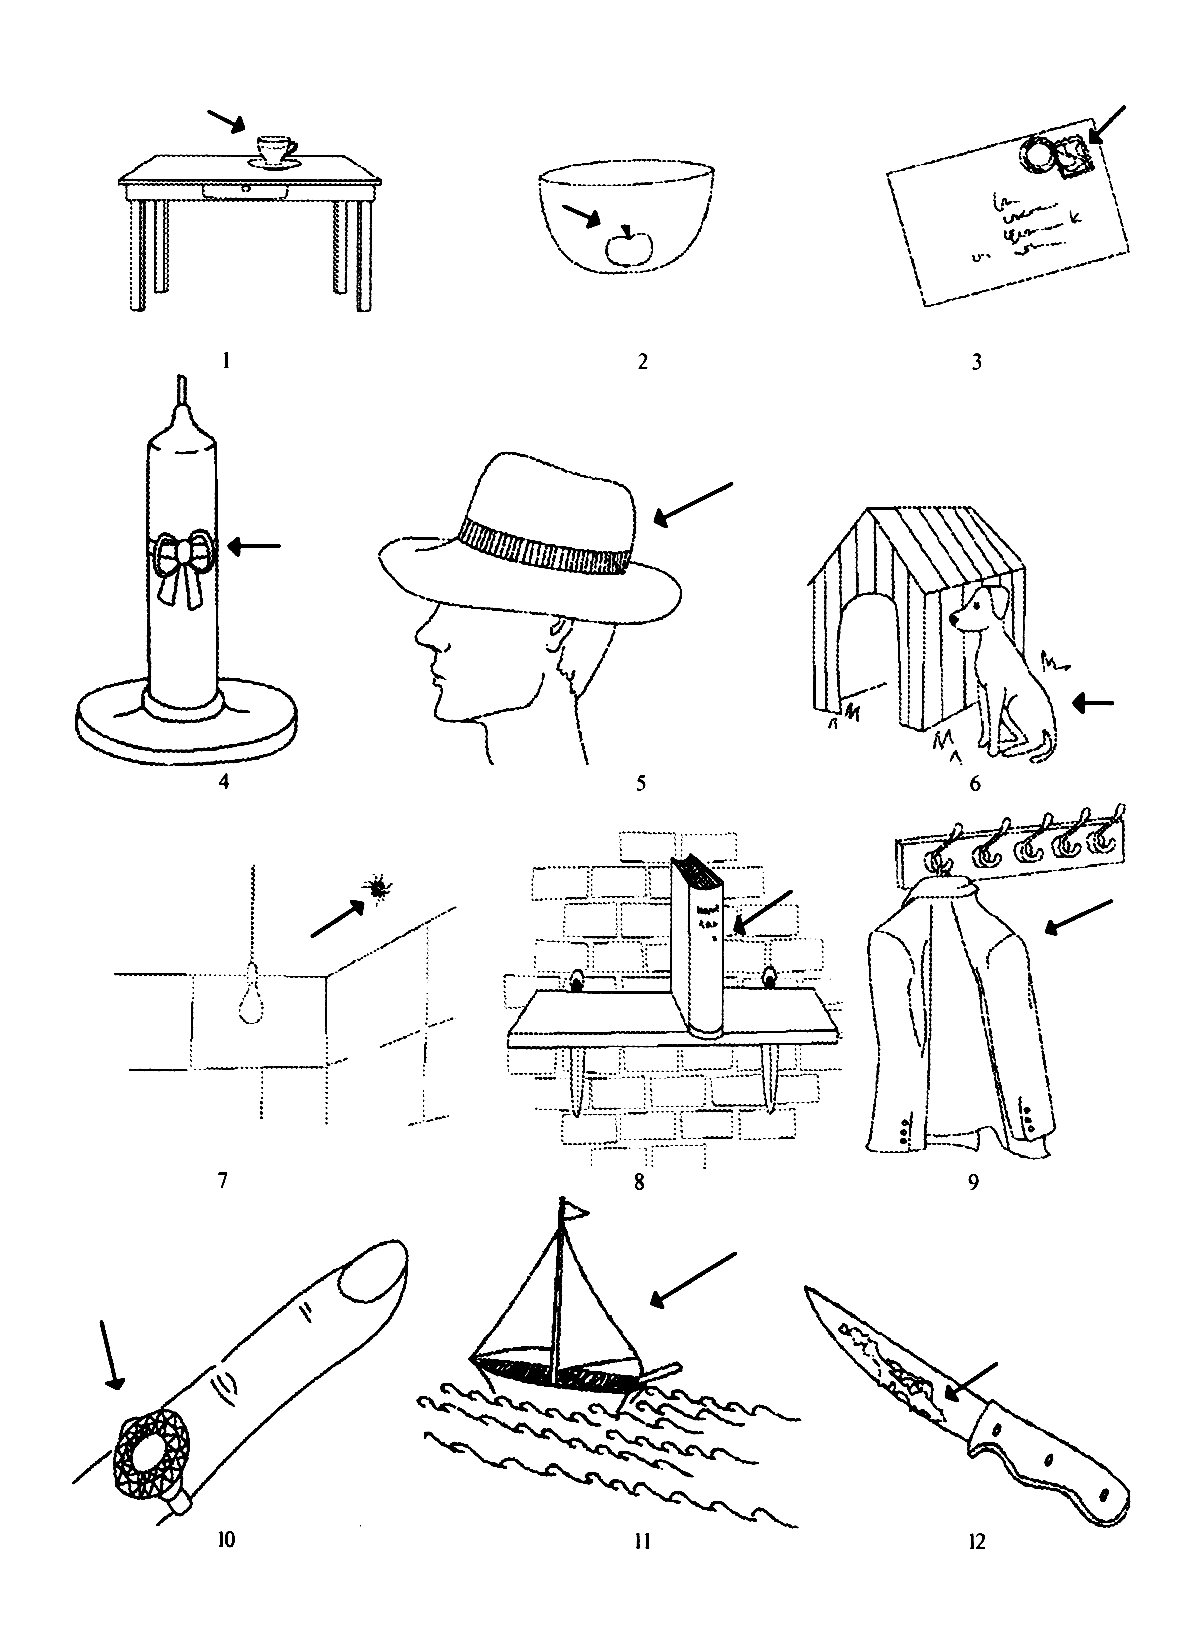
\includegraphics[width=3.5in]{Graphic/Pictures/BLC-1.jpg}
}
\qquad
\subfloat{
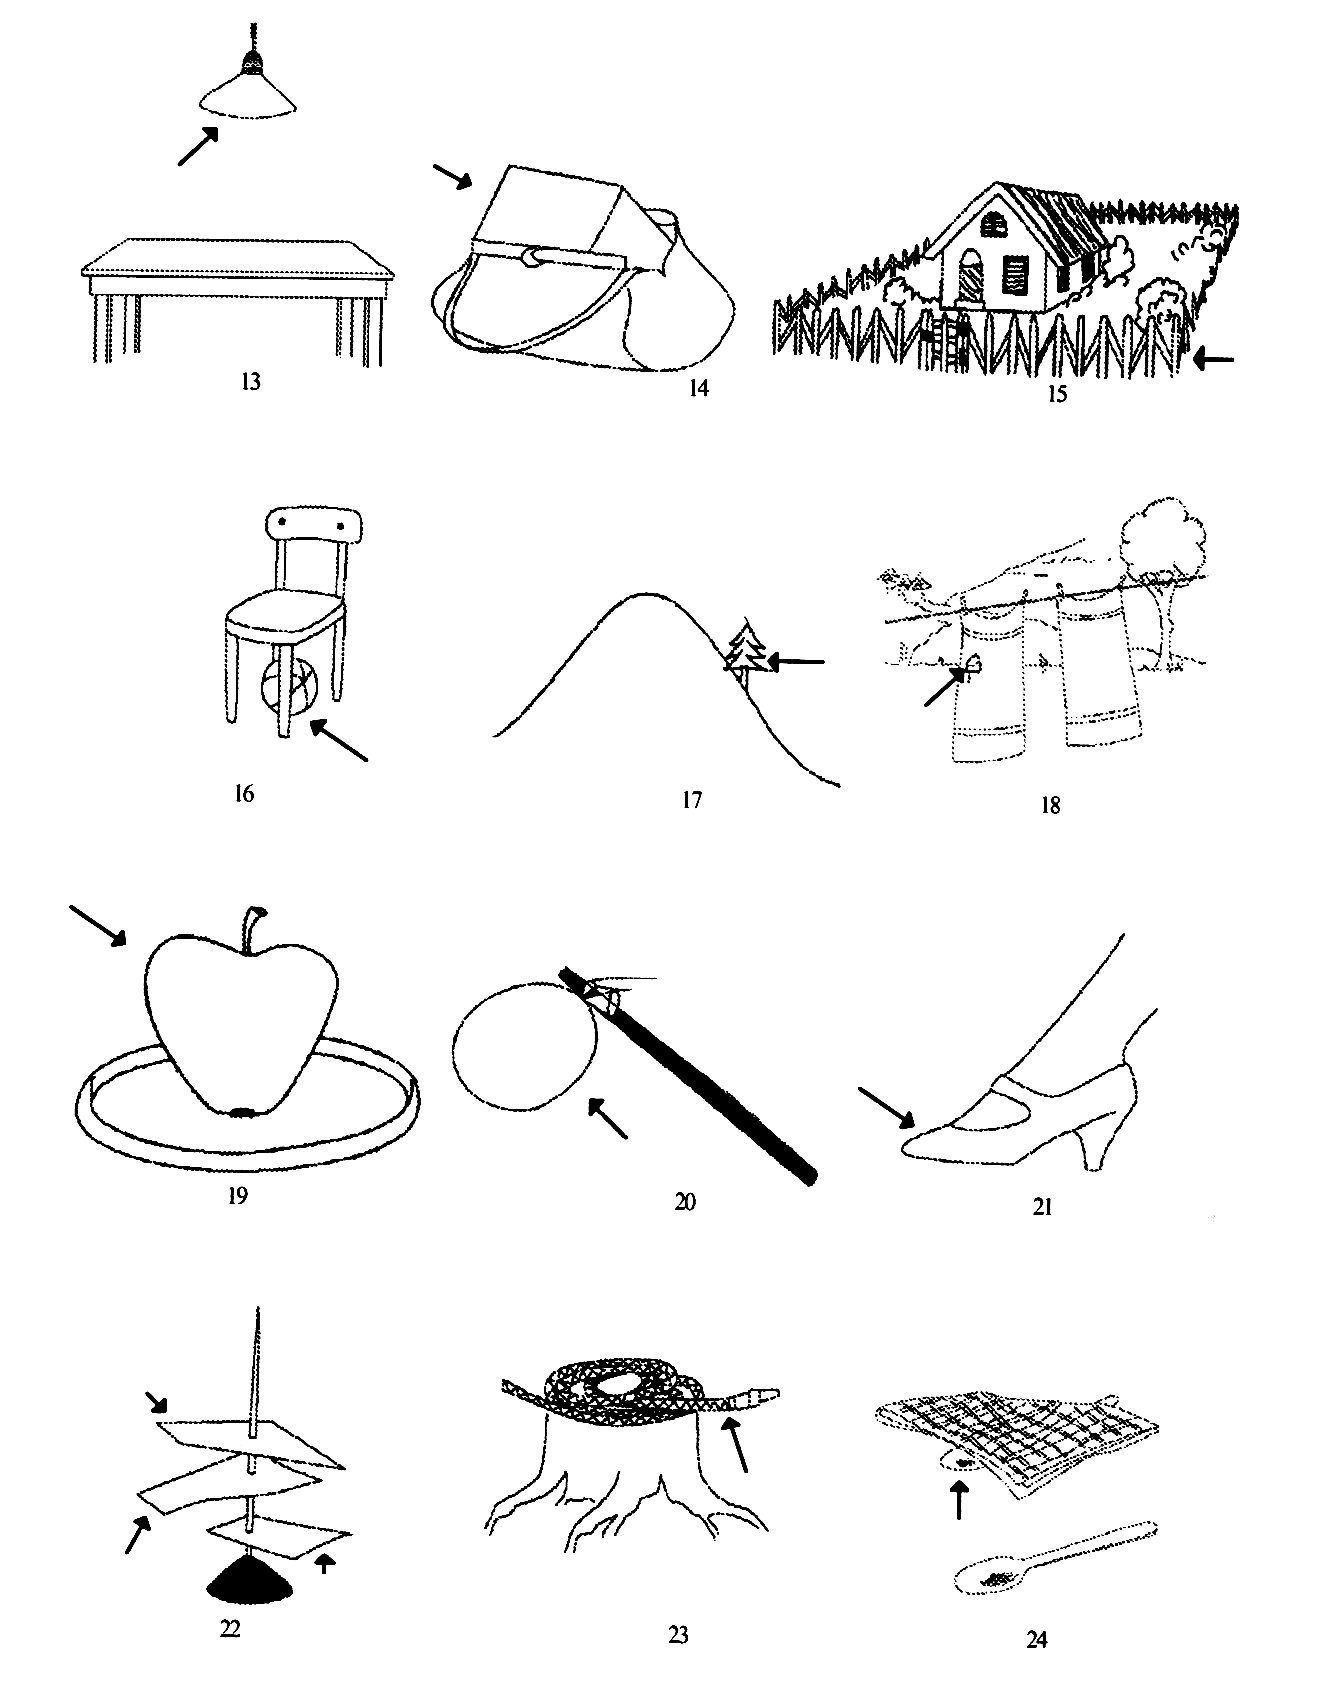
\includegraphics[width=3.5in]{Graphic/Pictures/BLC-2.jpg}
}
\caption[TRPS 1-24]{Topological Relations Picture Series: illustrations 1-24
(\textcopyright MPI, Nijmegen)
  \cite[570-71]{Levi06} \label{fig:TRPS-1-24}}
%\end{figure} 
\end{sidewaysfigure}


\begin{sidewaysfigure}
\subfloat{
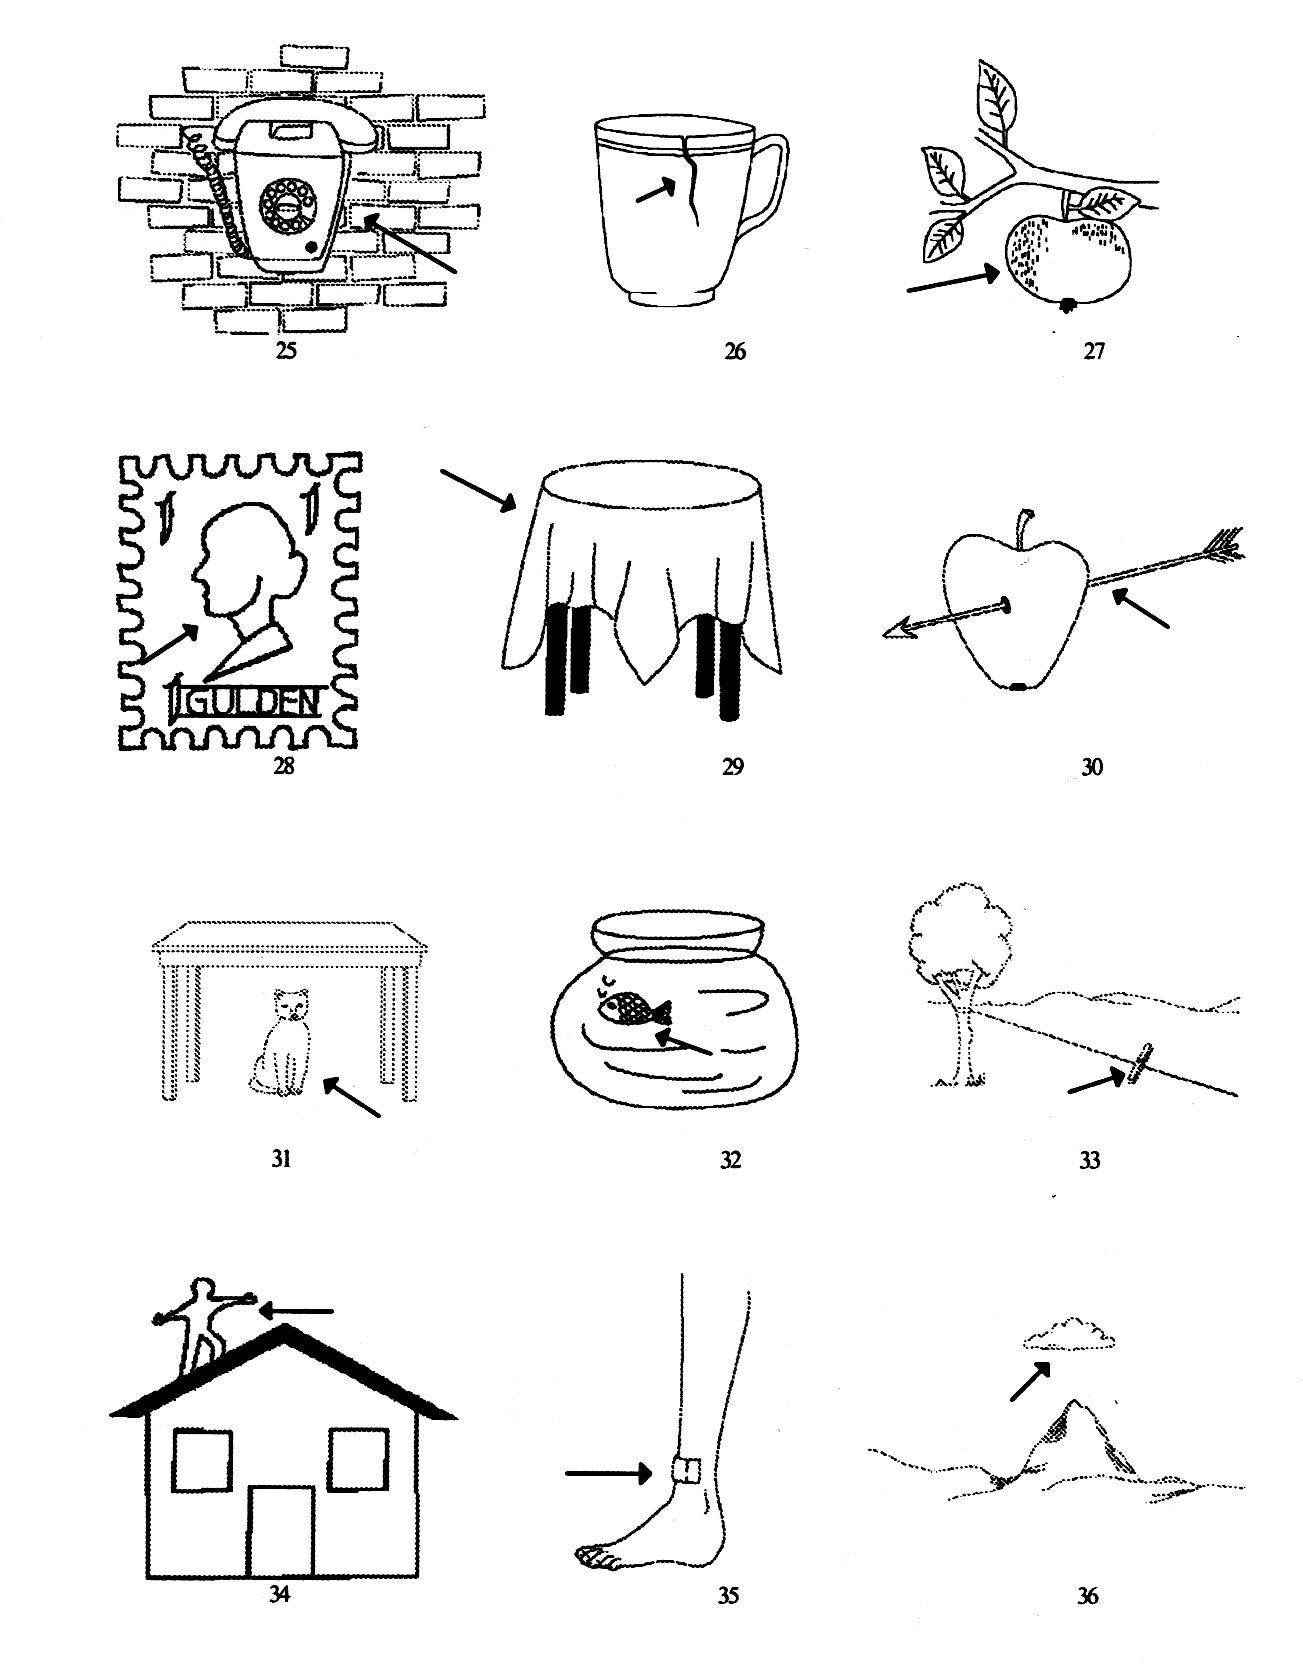
\includegraphics[width=3.5in]{Graphic/Pictures/BLC-3.jpg}
}
\qquad
\subfloat{
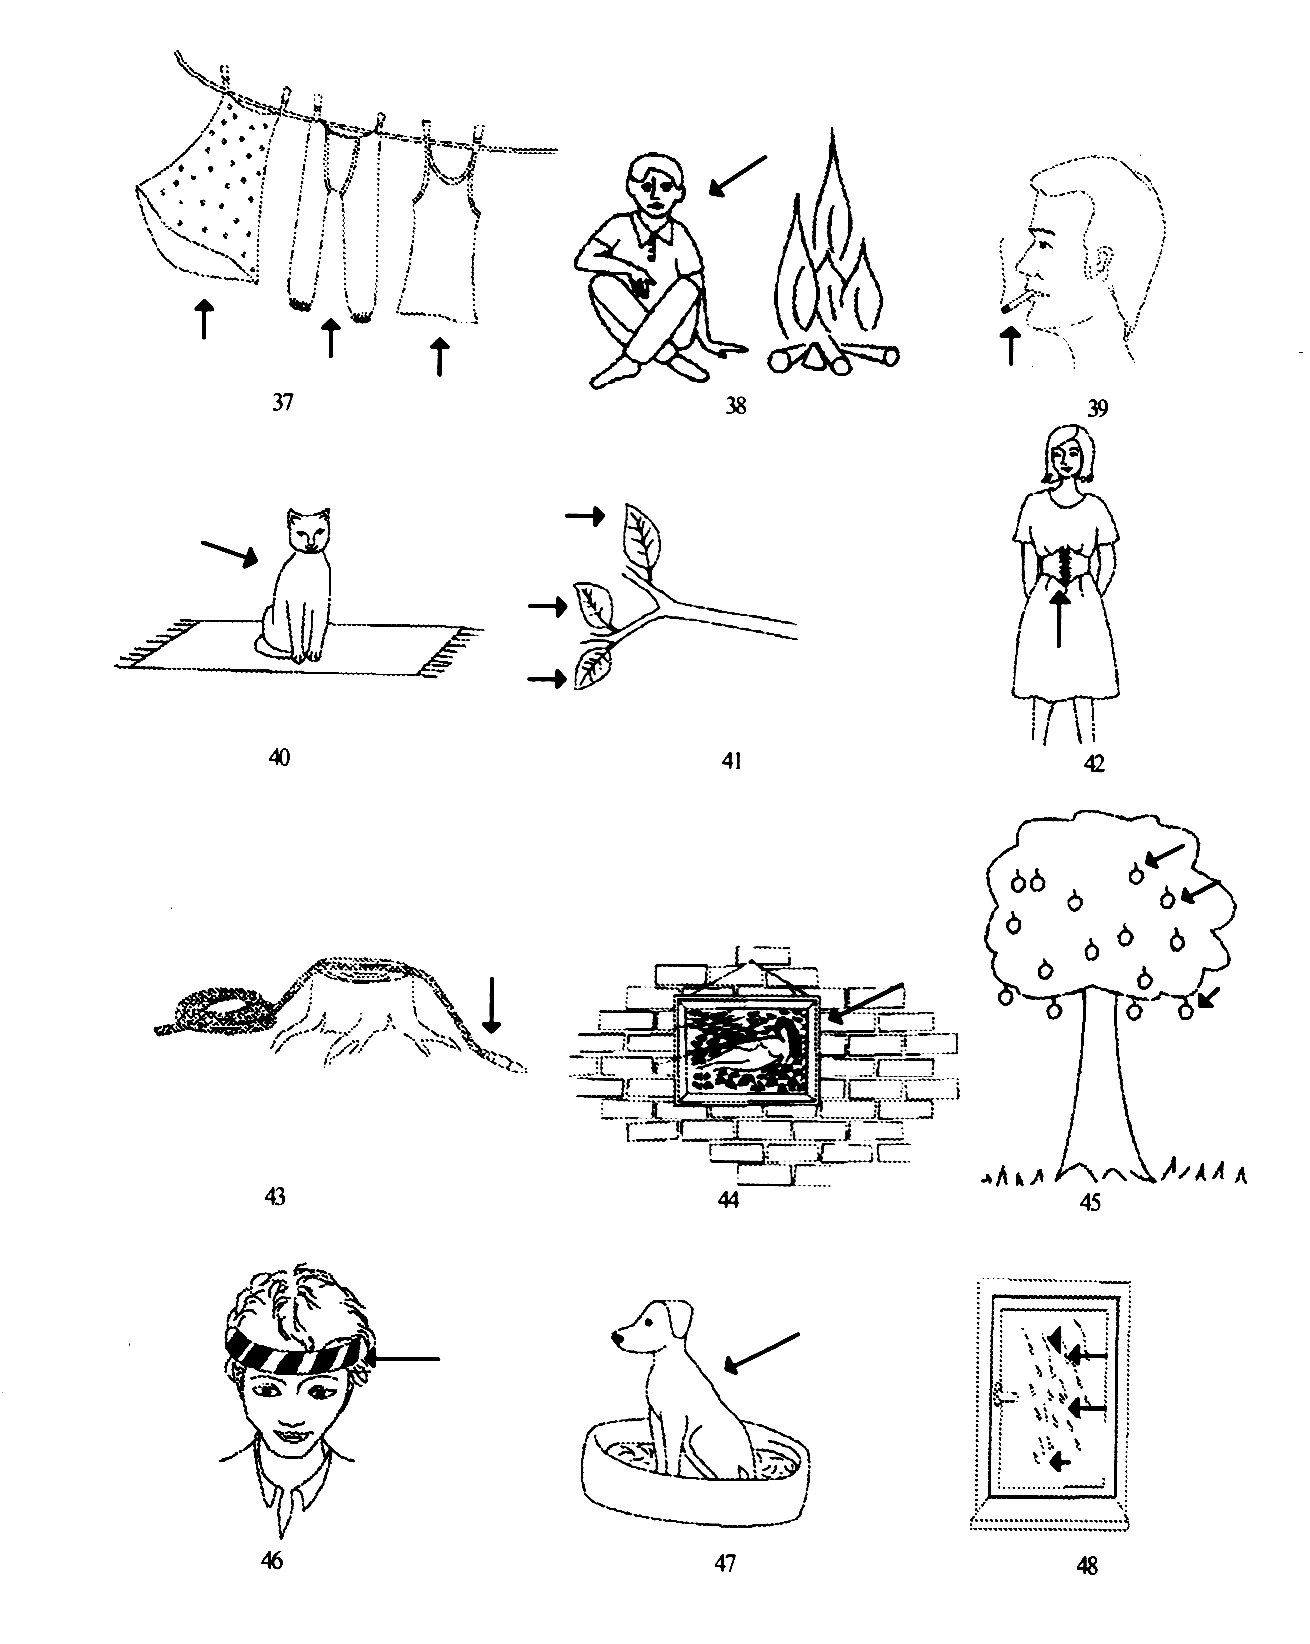
\includegraphics[width=3.5in]{Graphic/Pictures/BLC-4.jpg}
}
\caption[TRPS 25-48]{Topological Relations Picture Series: illustrations 25-48
(\textcopyright MPI, Nijmegen)
  \cite[572-73]{Levi06}  \label{fig:TRPS-25-48}}
\end{sidewaysfigure} 


\begin{sidewaysfigure}
\subfloat{
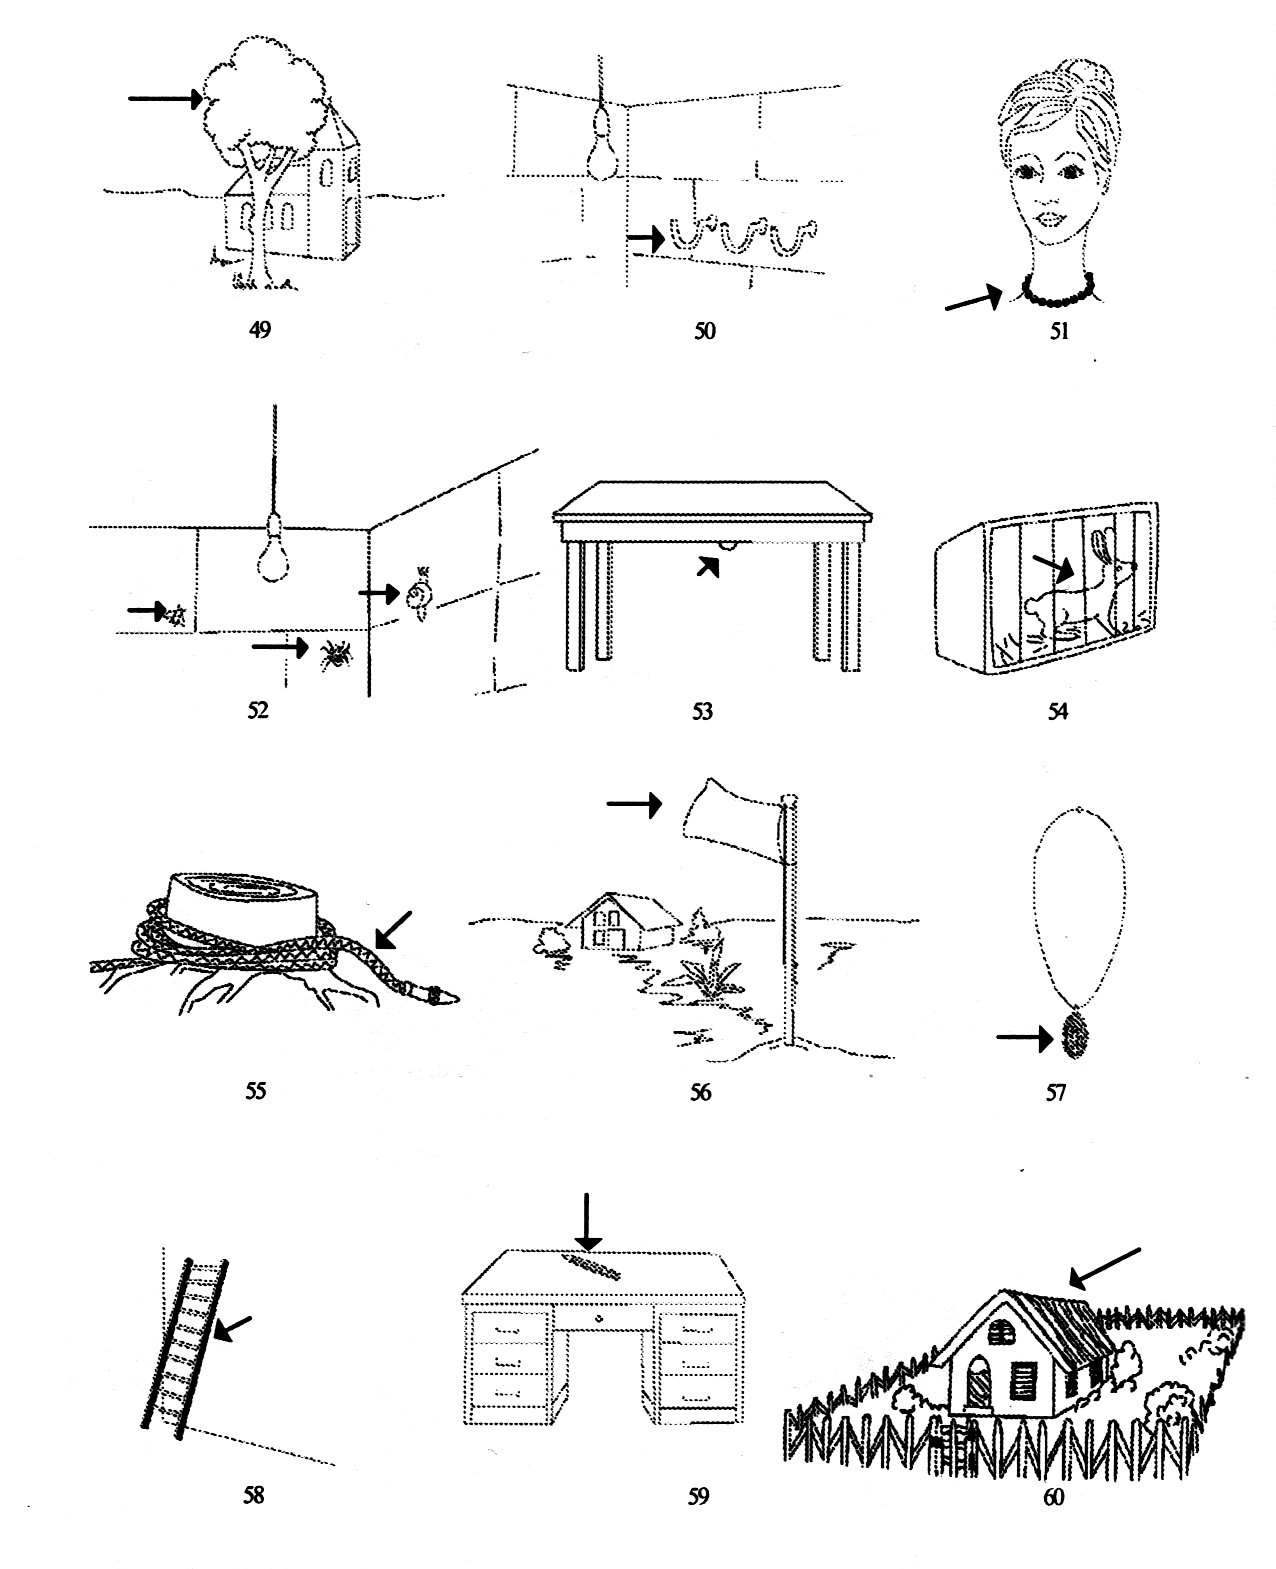
\includegraphics[width=3.5in]{Graphic/Pictures/BLC-5.jpg}
}
\qquad
\subfloat{
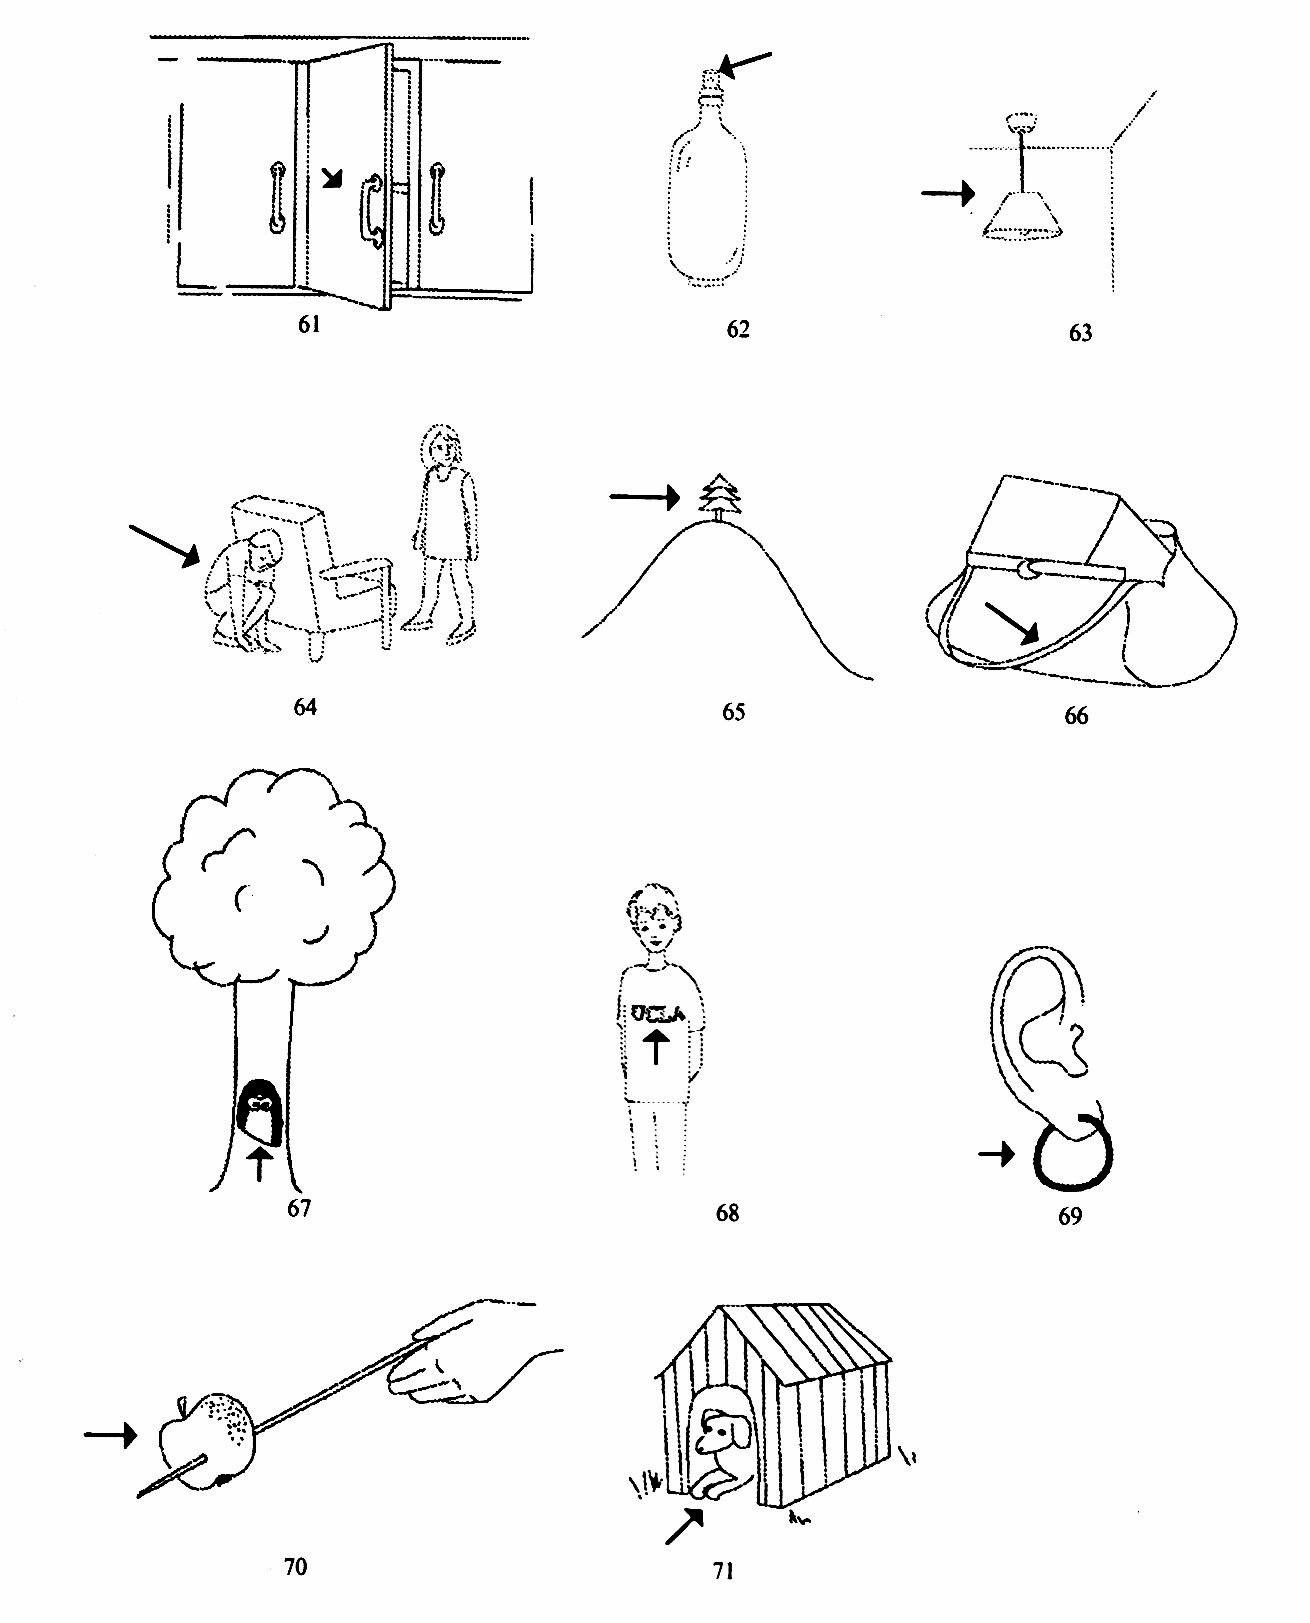
\includegraphics[width=3.5in]{Graphic/Pictures/BLC-6.jpg}
}
\caption[TRPS 49-71]{Topological Relations Picture Series: illustrations
 49-71  (\textcopyright MPI, Nijmegen) \cite[574-75]{Levi06}
\label{fig:TRPS-49-71}}
\end{sidewaysfigure}



\begin{sidewaysfigure}
\subfloat{
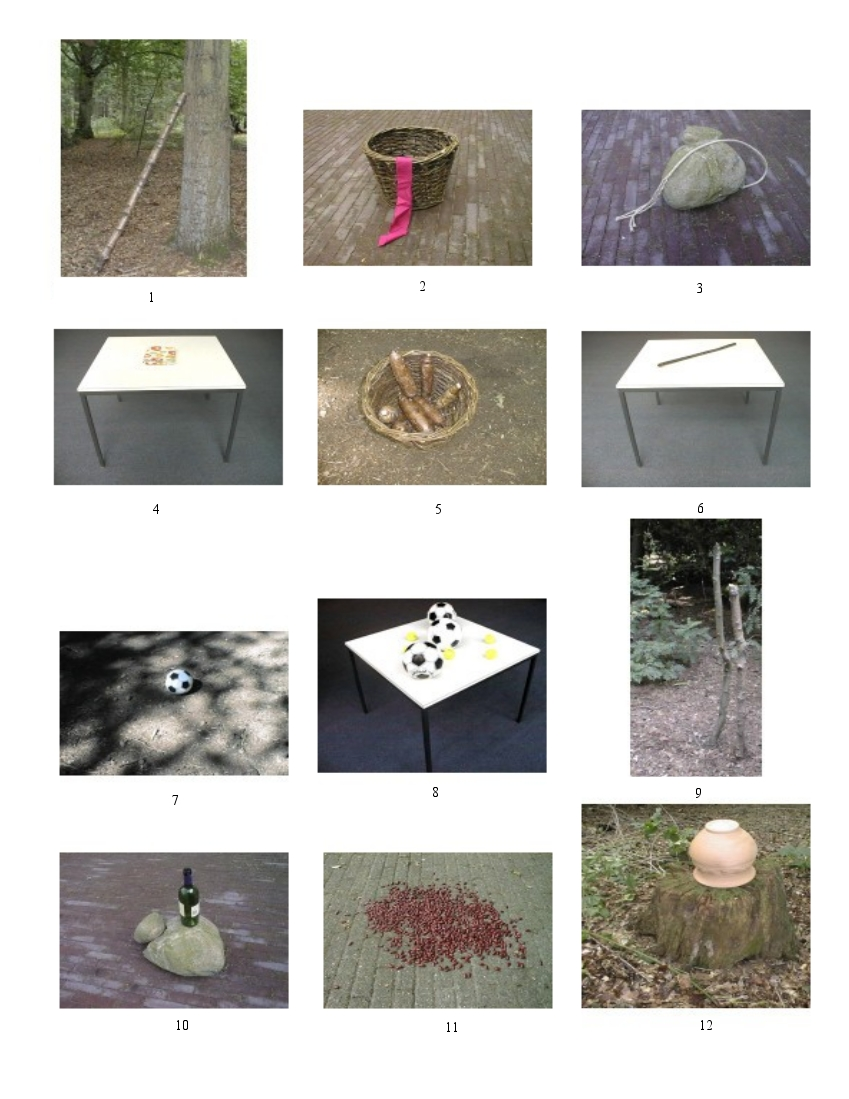
\includegraphics[width=3.5in]{Graphic/Pictures/PSPV-P1.jpg}
}
\qquad
\subfloat{
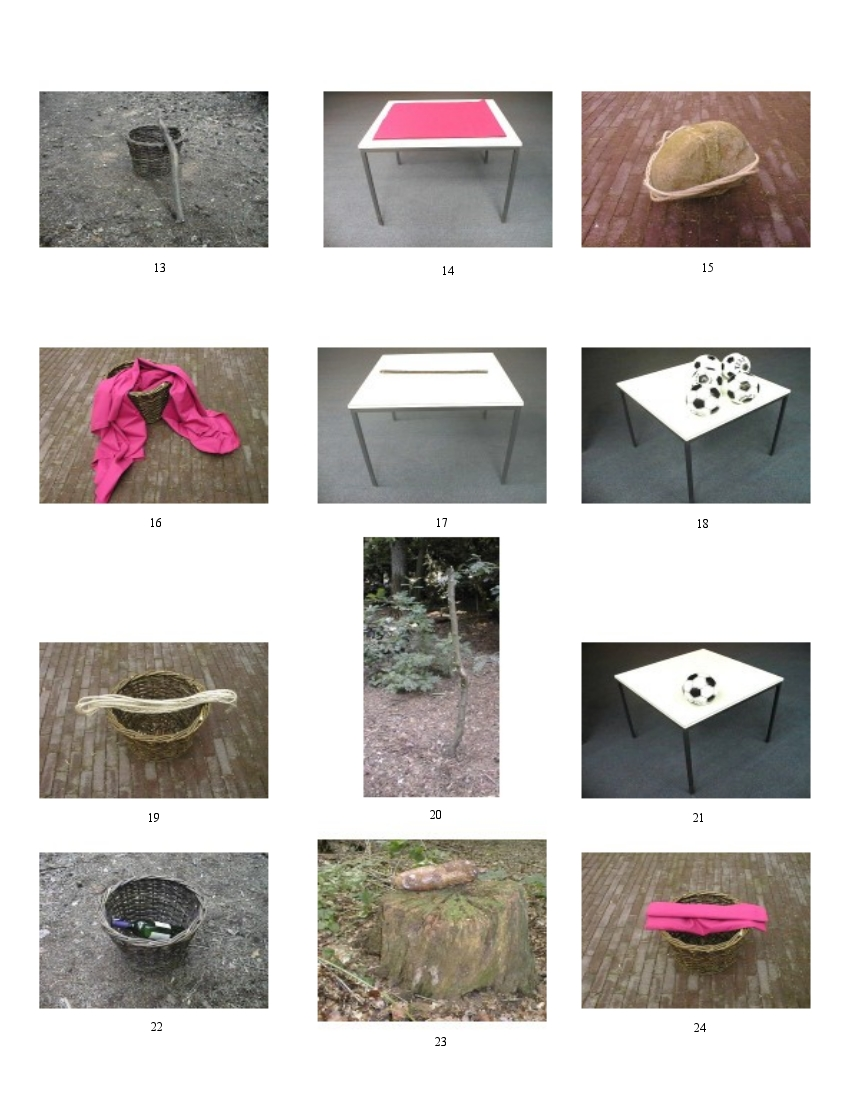
\includegraphics[width=3.5in]{Graphic/Pictures/PSPV-P2.jpg}
}
\caption[PSPV 1-24]{Picture Series for Positional Verbs: pictures
  1-24 (\textcopyright MPI, Nijmegen) \label{fig:PSPV-1-24}}
\end{sidewaysfigure}

\begin{sidewaysfigure}
\subfloat{
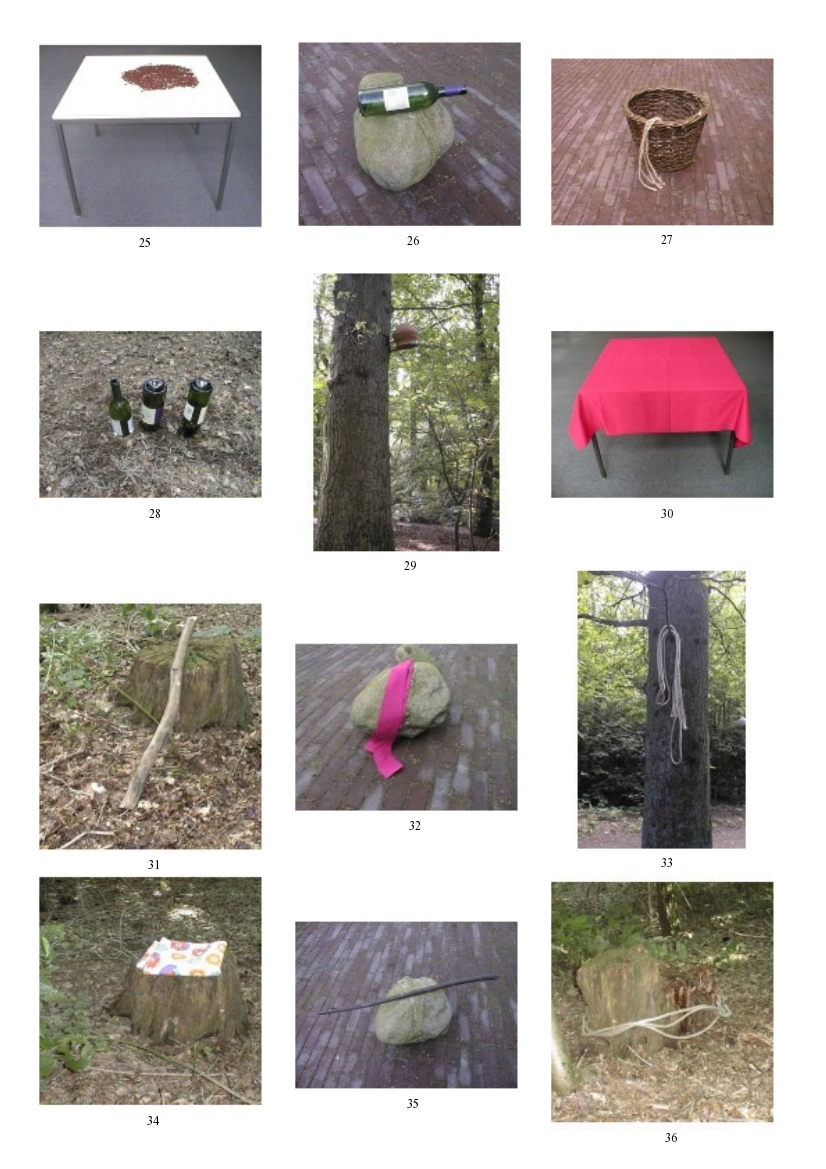
\includegraphics[width=3.5in]{Graphic/Pictures/PSPV-P3.jpg}
}
\qquad
\subfloat{
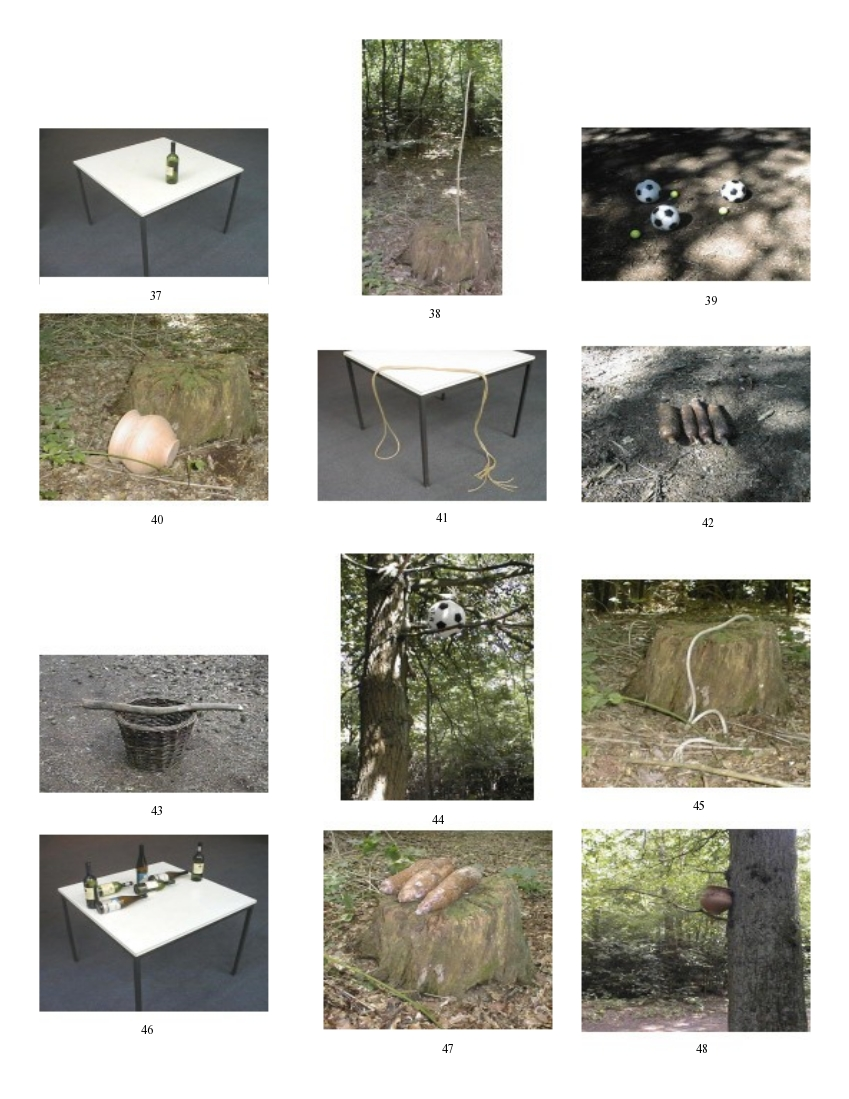
\includegraphics[width=3.5in]{Graphic/Pictures/PSPV-P4.jpg}
}
\caption[PSPV 25-48]{Picture Series for Positional Verbs: pictures
  25-48 (\textcopyright MPI, Nijmegen) \label{fig:PSPV-25-48}}
\end{sidewaysfigure}


\begin{sidewaysfigure}
\subfloat{
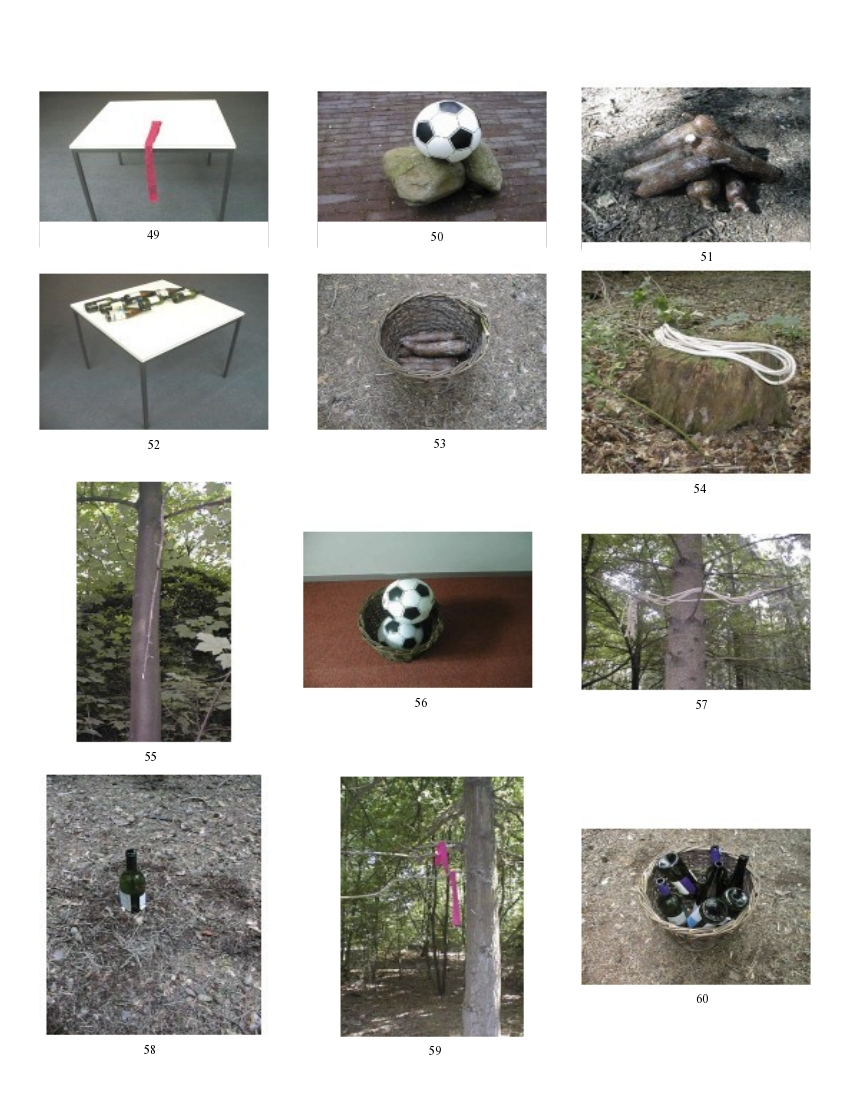
\includegraphics[width=3.5in]{Graphic/Pictures/PSPV-P5.jpg}
}
\qquad
\subfloat{
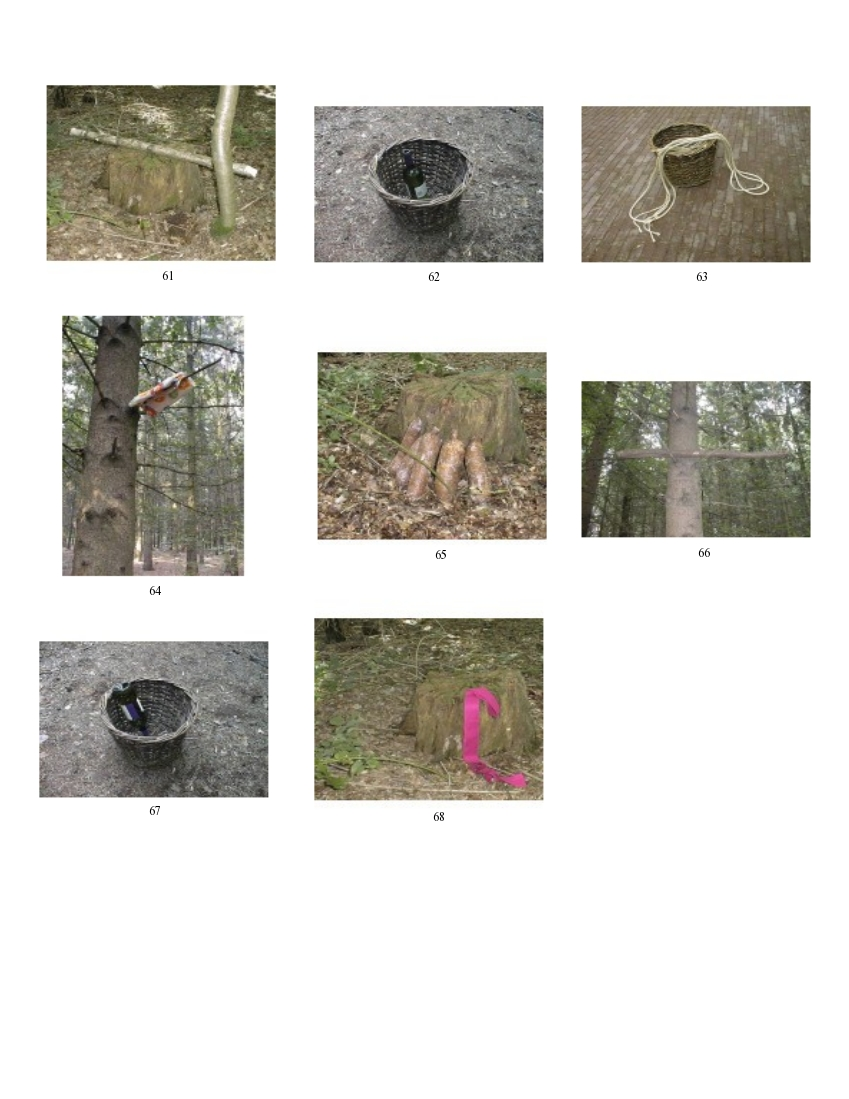
\includegraphics[width=3.5in]{Graphic/Pictures/PSPV-P6.jpg}
}
\caption[PSPV 49-68]{Picture Series for Positional Verbs: pictures
  49-68 (\textcopyright MPI, Nijmegen) \label{fig:PSPV-49-68}}
\end{sidewaysfigure}


\pagebreak

\begin{sidewaysfigure}
\subfloat{
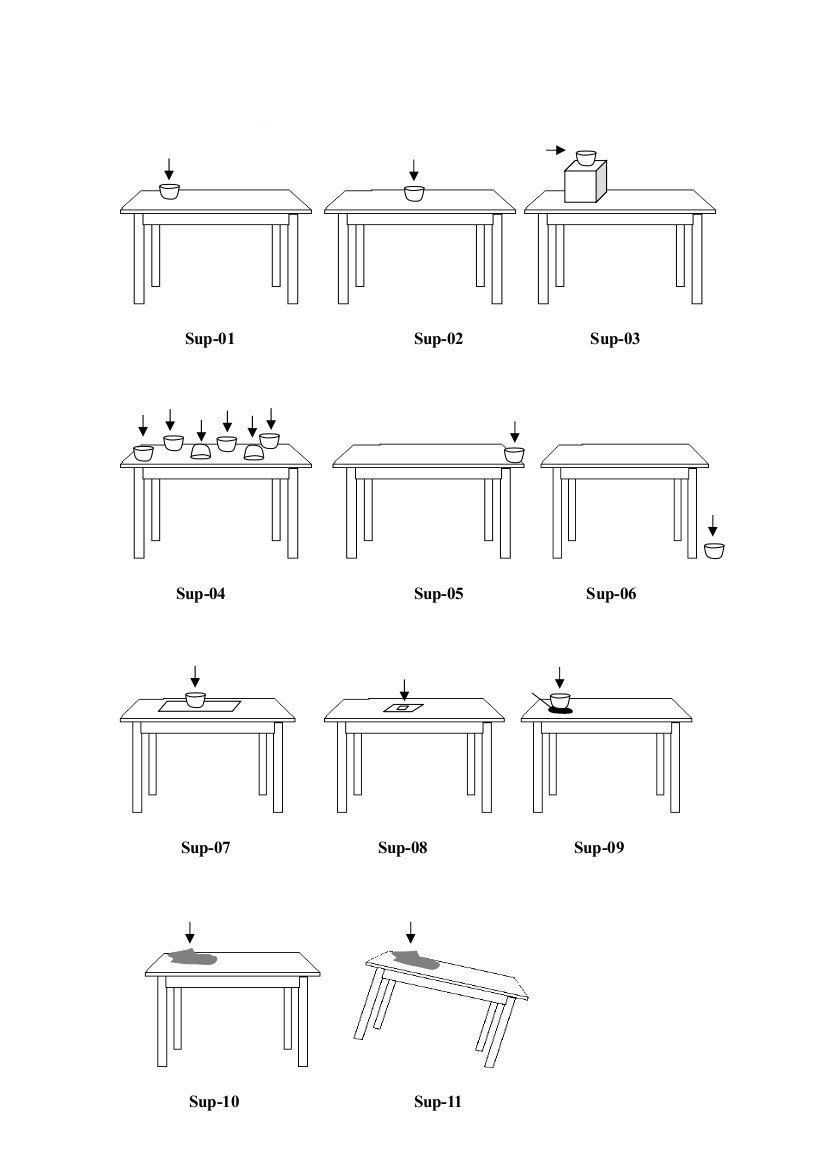
\includegraphics[width=3.5in]{Graphic/Pictures/Supp-1.jpg}
}
\qquad
\subfloat{
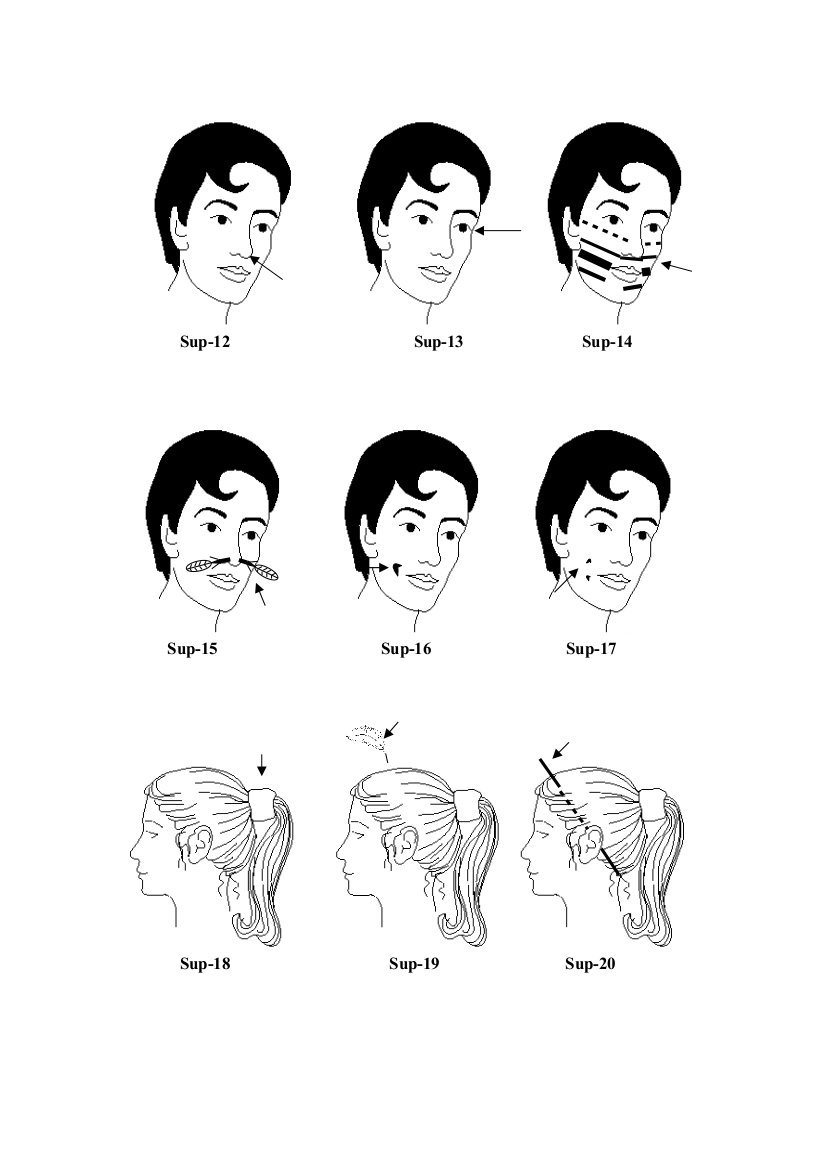
\includegraphics[width=3.5in]{Graphic/Pictures/Supp-2.jpg}
}
\caption[SPS 1-20]{Support Picture Series: pictures
  1-20 (\textcopyright MPI, Nijmegen) \label{fig:Support-1-20}}
\end{sidewaysfigure}


\begin{sidewaysfigure}
\subfloat{
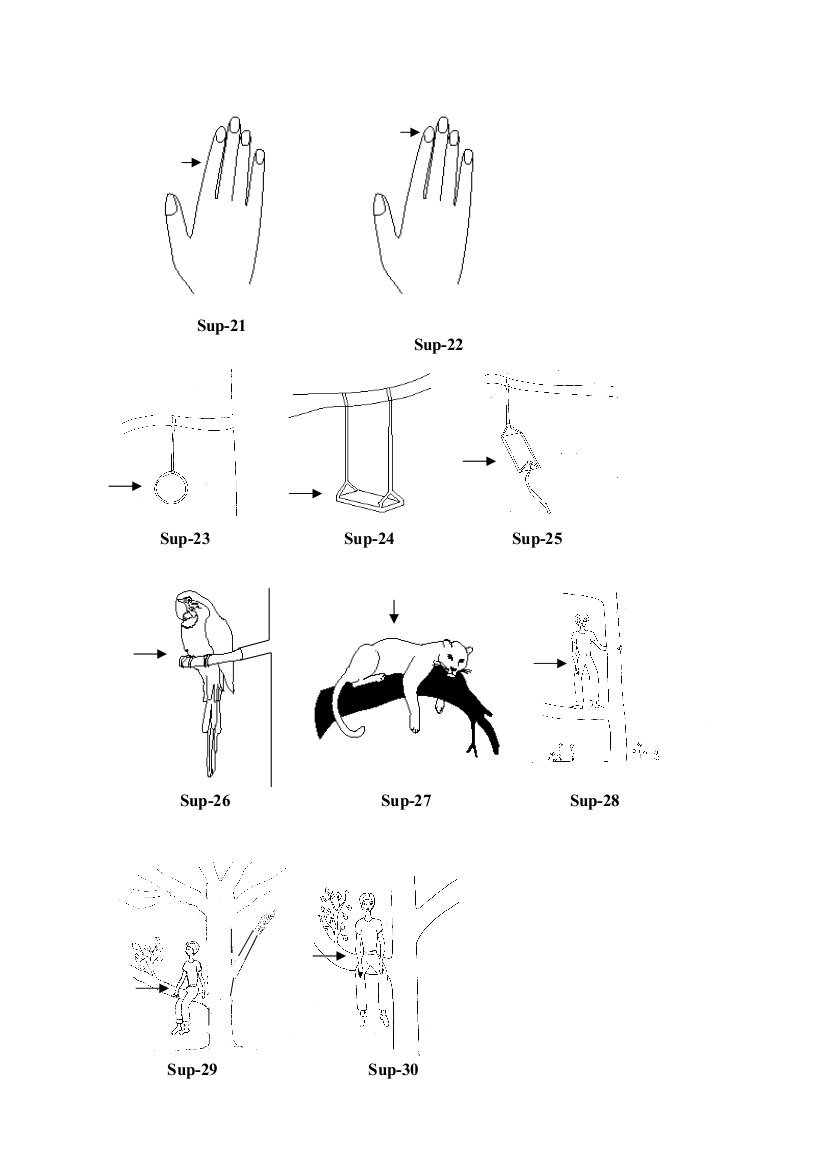
\includegraphics[width=3.5in]{Graphic/Pictures/Supp-3.jpg}
}
\qquad
\subfloat{
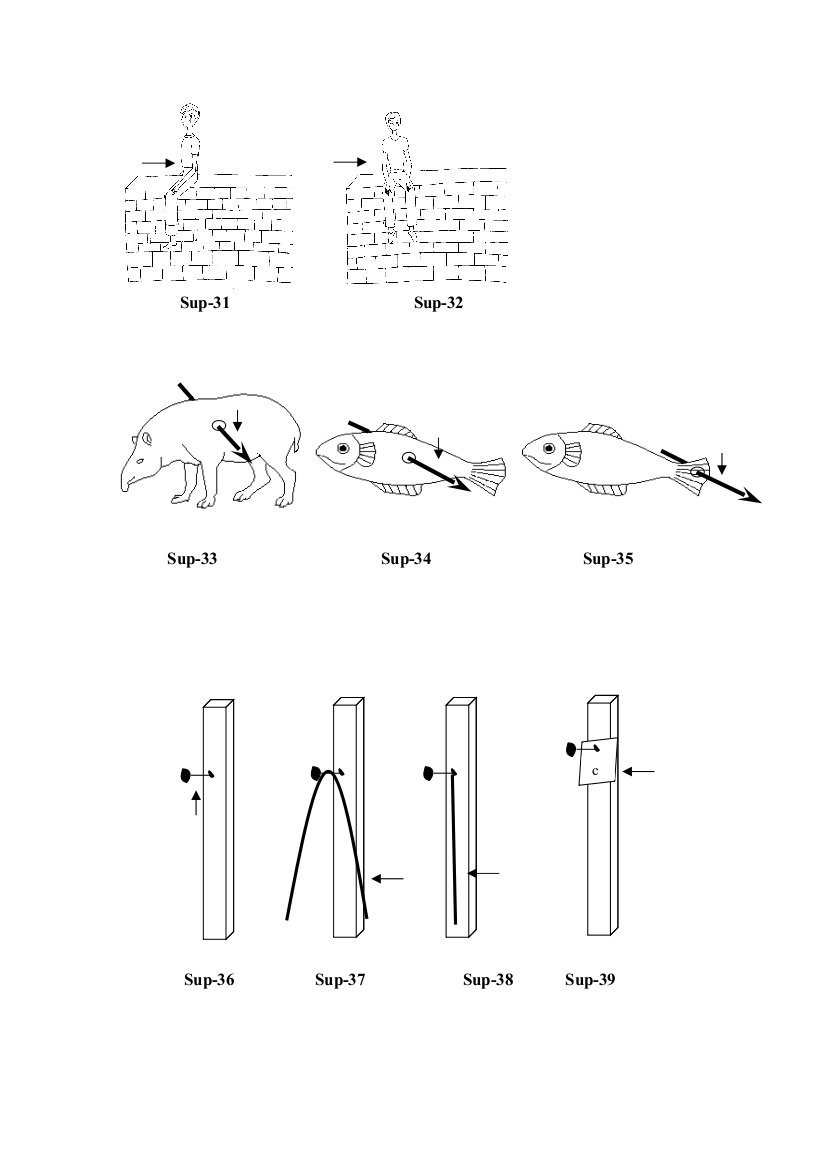
\includegraphics[width=3.5in]{Graphic/Pictures/Supp-4.jpg}
}
\caption[SPS 21-39]{Support Picture Series: pictures
  21-39 (\textcopyright MPI, Nijmegen) \label{fig:Support-21-39}}
\end{sidewaysfigure}


\begin{sidewaysfigure}
\subfloat{
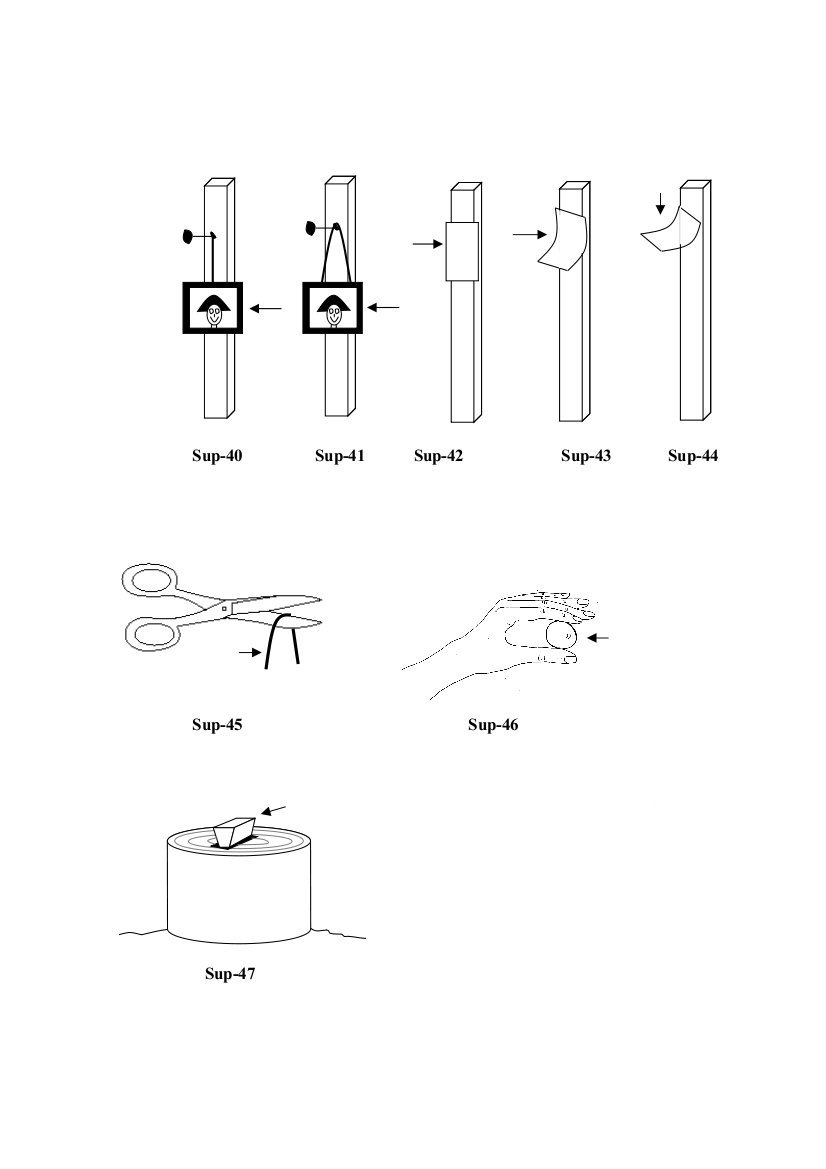
\includegraphics[width=3.5in]{Graphic/Pictures/Supp-5.jpg}
}
\qquad
\subfloat{
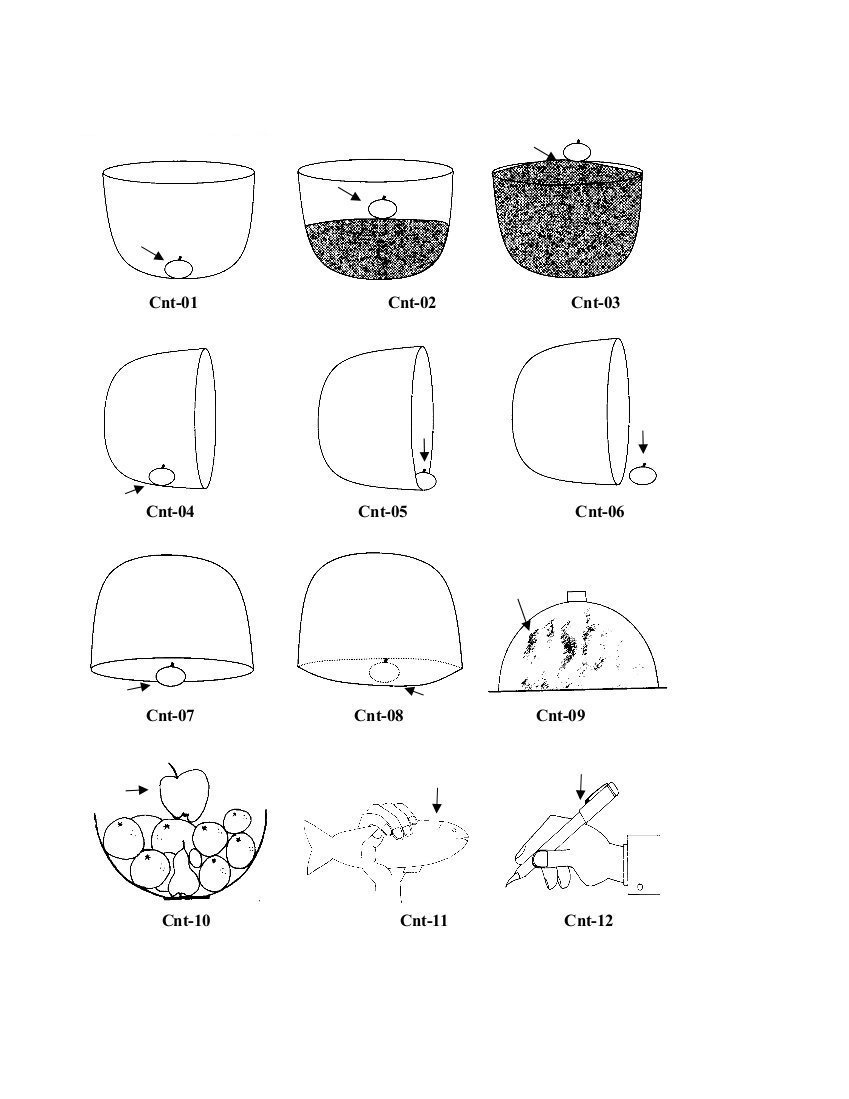
\includegraphics[width=3.5in]{Graphic/Pictures/CPS-1.jpg}
}
\caption[SPS 40-47 and CPS 1-12]{Support Picture Series: pictures
  40-47. Containment Picture Series: pictures 1-12 (\textcopyright MPI,
Nijmegen)
\label{fig:Support-20-27-CPS-1-12}}
\end{sidewaysfigure}


\begin{sidewaysfigure}
\subfloat{
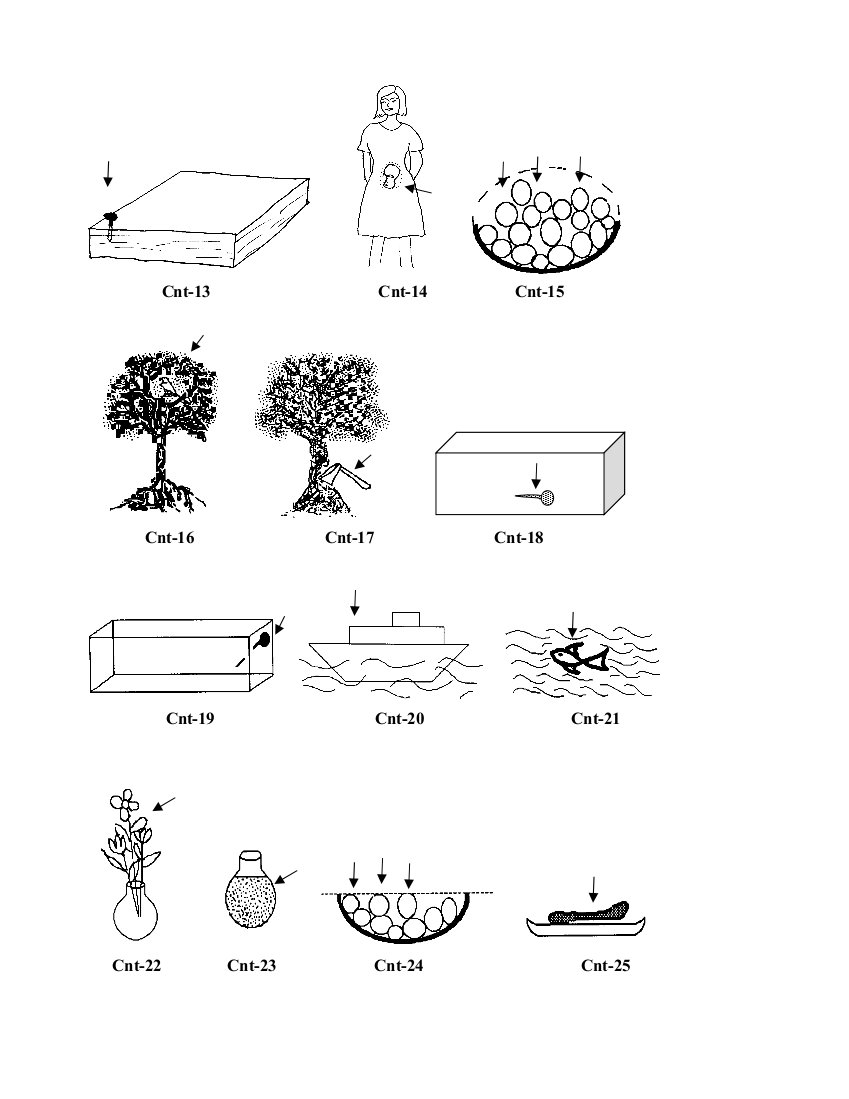
\includegraphics[width=3.5in]{Graphic/Pictures/CPS-2.jpg}
}
\qquad
\subfloat{
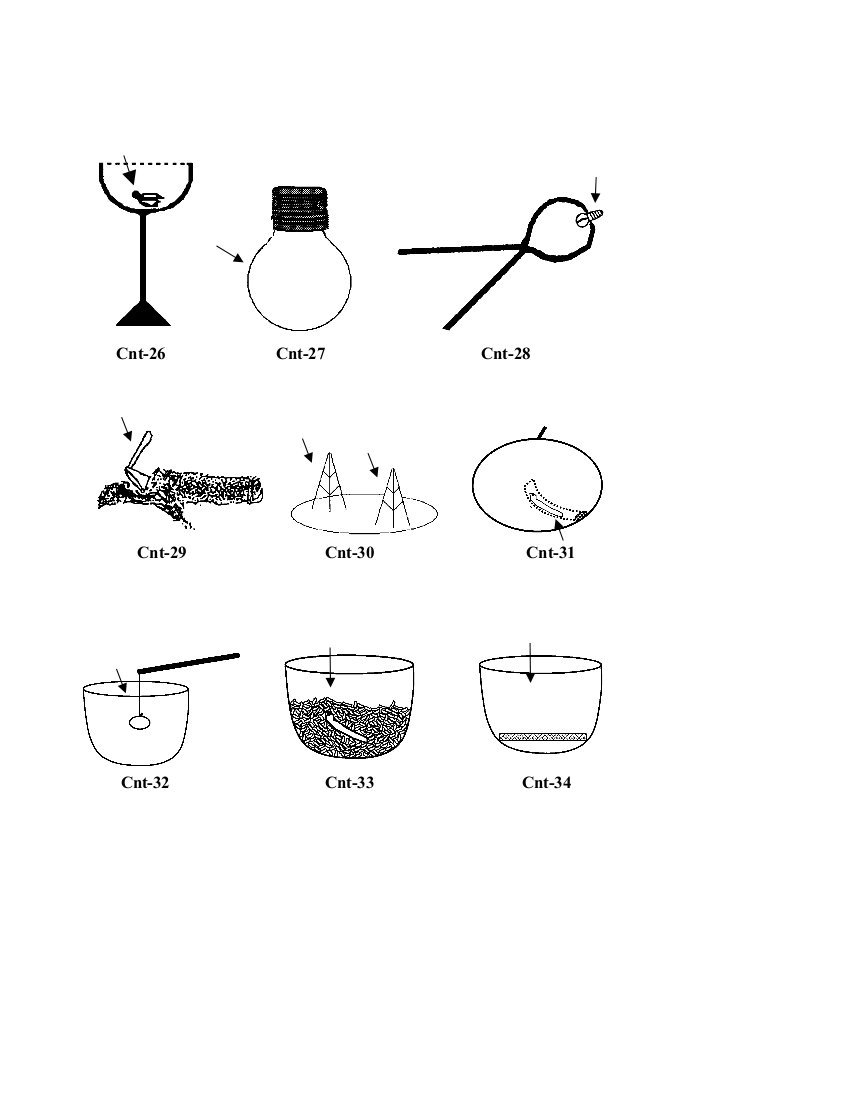
\includegraphics[width=3.5in]{Graphic/Pictures/CPS-3.jpg}
}
\caption[CPS 13-34]{Containment Picture Series: pictures 
  13-34 (\textcopyright MPI, Nijmegen)  \label{fig:CPS-13-34}}
\end{sidewaysfigure}


\begin{sidewaysfigure}
\subfloat{
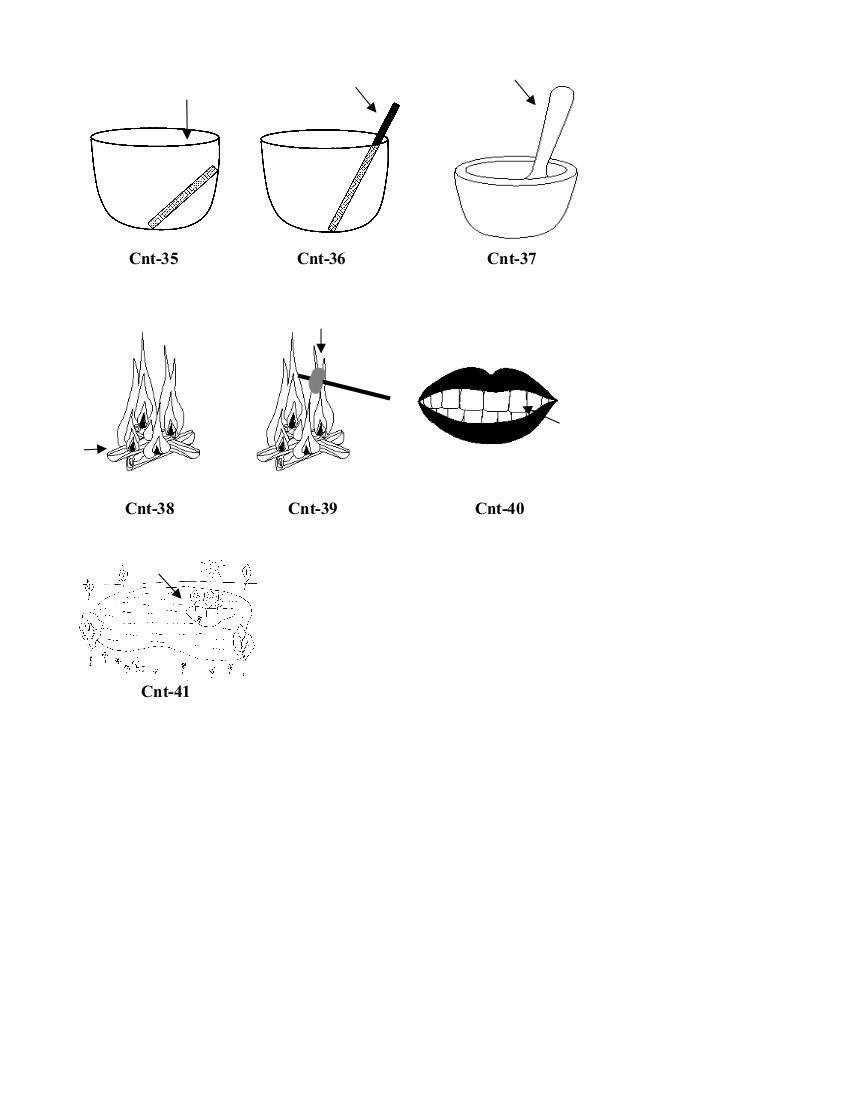
\includegraphics[width=3.5in]{Graphic/Pictures/CPS-4.jpg}
}
\qquad
\subfloat{
}
\caption[CPS 35-41]{Containment Picture Series: pictures 
  35-41 (\textcopyright MPI, Nijmegen) \label{fig:CPS-35-41}}
\end{sidewaysfigure} 